\documentclass[10pt]{article}
\usepackage[margin=2.2cm]{geometry}
\usepackage{booktabs,longtable,graphicx,array}
\usepackage[hidelinks]{hyperref}
\setlength{\tabcolsep}{4pt}
\newcommand{\stackcell}[1]{\begin{tabular}[t]{@{}l@{}}#1\end{tabular}}
\title{tropical: ThreeSumDecision}
\date{2026-10-26T03:54:11}
\begin{document}
\maketitle

\section{Key results}
This report covers 240 runs (5 seeds; 0 diverged) under frozen hash \texttt{096095567af4}.
\paragraph{Where to look.} The headline metric is \texttt{ood\_len\_f1} (higher is better).
\autoref{fig:ood_len_f1} plots it against \texttt{fishr\_lambda}.
\autoref{tab:summary-ood_len_f1} gives every cell's mean with its 95\% bootstrap CI.
\autoref{tab:control-ood_len_f1} compares each level with the control.
\autoref{tab:trend-ood_len_f1} gives the trend.
\autoref{tab:paired-ood_len_f1} gives the paired contrasts.
Its tests take the rank-based path: more than 20\% of values within 0.01 of a bound (0, 1).
Cells are compared within a seed: a seed index fixes the data and the initialization.
Comparisons are marked significant at $p < 0.05$ after the stated correction.

\subsection{\texttt{ood\_len\_f1}}
\begin{figure}[tbp]
\centering
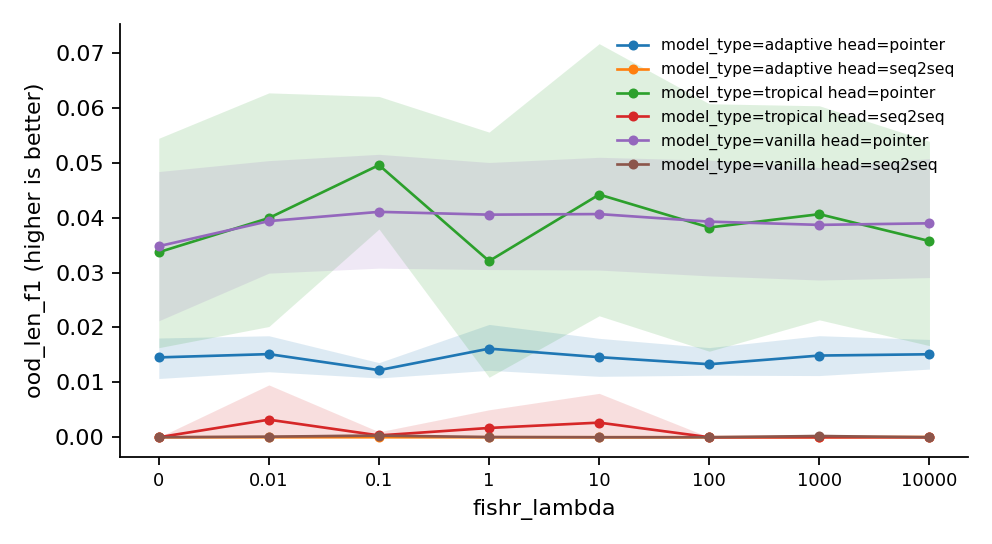
\includegraphics[width=\textwidth]{metric_ood_len_f1.png}
\caption{\texttt{ood\_len\_f1} against \texttt{fishr\_lambda}: the mean over seeds with a 95\% bootstrap CI, one line per combination of the other factors.}
\label{fig:ood_len_f1}
\end{figure}

{\small
\begin{longtable}{lllrlrrr}
\caption{\texttt{ood\_len\_f1} per cell: mean, 95\% bootstrap CI, SD, seeds, diverged runs.}\label{tab:summary-ood_len_f1}\\
\toprule
\texttt{model\_type} & \texttt{head} & \texttt{fishr\_lambda} & mean & 95\% CI & SD & $n$ & div.\\
\midrule
\endhead
adaptive & pointer & 0 & 0.01455 & [0.0107, 0.0181] & 0.00479 & 5 & 0\\
adaptive & pointer & 0.01 & 0.01514 & [0.0119, 0.0185] & 0.0042 & 5 & 0\\
adaptive & pointer & 0.1 & 0.01222 & [0.0108, 0.0136] & 0.00182 & 5 & 0\\
adaptive & pointer & 1 & 0.01614 & [0.0122, 0.0206] & 0.00537 & 5 & 0\\
adaptive & pointer & 10 & 0.01459 & [0.0111, 0.018] & 0.00447 & 5 & 0\\
adaptive & pointer & 100 & 0.0133 & [0.0113, 0.0163] & 0.00332 & 5 & 0\\
adaptive & pointer & 1000 & 0.01488 & [0.0112, 0.0185] & 0.00468 & 5 & 0\\
adaptive & pointer & 1e+04 & 0.01512 & [0.0124, 0.0178] & 0.00357 & 5 & 0\\
adaptive & seq2seq & 0 & 0 & [0, 0] & 0 & 5 & 0\\
adaptive & seq2seq & 0.01 & 0 & [0, 0] & 0 & 5 & 0\\
adaptive & seq2seq & 0.1 & 0 & [0, 0] & 0 & 5 & 0\\
adaptive & seq2seq & 1 & 0 & [0, 0] & 0 & 5 & 0\\
adaptive & seq2seq & 10 & 0 & [0, 0] & 0 & 5 & 0\\
adaptive & seq2seq & 100 & 0 & [0, 0] & 0 & 5 & 0\\
adaptive & seq2seq & 1000 & 0 & [0, 0] & 0 & 5 & 0\\
adaptive & seq2seq & 1e+04 & $3.743\times10^{-5}$ & [0, $1.12\times10^{-4}$] & $8.37\times10^{-5}$ & 5 & 0\\
tropical & pointer & 0 & 0.03371 & [0.0163, 0.0545] & 0.0256 & 5 & 0\\
tropical & pointer & 0.01 & 0.03993 & [0.0202, 0.0627] & 0.0266 & 5 & 0\\
tropical & pointer & 0.1 & 0.04958 & [0.0379, 0.0621] & 0.0162 & 5 & 0\\
tropical & pointer & 1 & 0.03209 & [0.0109, 0.0556] & 0.0287 & 5 & 0\\
tropical & pointer & 10 & 0.04421 & [0.0221, 0.0717] & 0.0328 & 5 & 0\\
tropical & pointer & 100 & 0.03821 & [0.0157, 0.0607] & 0.0303 & 5 & 0\\
tropical & pointer & 1000 & 0.04064 & [0.0214, 0.0604] & 0.026 & 5 & 0\\
tropical & pointer & 1e+04 & 0.03573 & [0.0167, 0.0539] & 0.0248 & 5 & 0\\
tropical & seq2seq & 0 & 0 & [0, 0] & 0 & 5 & 0\\
tropical & seq2seq & 0.01 & 0.003202 & [0, 0.00953] & 0.00706 & 5 & 0\\
tropical & seq2seq & 0.1 & $3.299\times10^{-4}$ & [0, $9.90\times10^{-4}$] & $7.38\times10^{-4}$ & 5 & 0\\
tropical & seq2seq & 1 & 0.001692 & [0, 0.005] & 0.00368 & 5 & 0\\
tropical & seq2seq & 10 & 0.002665 & [0, 0.008] & 0.00596 & 5 & 0\\
tropical & seq2seq & 100 & 0 & [0, 0] & 0 & 5 & 0\\
tropical & seq2seq & 1000 & 0 & [0, 0] & 0 & 5 & 0\\
tropical & seq2seq & 1e+04 & 0 & [0, 0] & 0 & 5 & 0\\
vanilla & pointer & 0 & 0.0348 & [0.0212, 0.0484] & 0.0173 & 5 & 0\\
vanilla & pointer & 0.01 & 0.03937 & [0.0299, 0.0504] & 0.0131 & 5 & 0\\
vanilla & pointer & 0.1 & 0.04106 & [0.0308, 0.0515] & 0.0133 & 5 & 0\\
vanilla & pointer & 1 & 0.04055 & [0.0305, 0.05] & 0.0131 & 5 & 0\\
vanilla & pointer & 10 & 0.04065 & [0.0305, 0.051] & 0.0127 & 5 & 0\\
vanilla & pointer & 100 & 0.03928 & [0.0294, 0.0505] & 0.0132 & 5 & 0\\
vanilla & pointer & 1000 & 0.03868 & [0.0286, 0.0491] & 0.0134 & 5 & 0\\
vanilla & pointer & 1e+04 & 0.03897 & [0.0291, 0.0508] & 0.0137 & 5 & 0\\
vanilla & seq2seq & 0 & 0 & [0, 0] & 0 & 5 & 0\\
vanilla & seq2seq & 0.01 & $1.100\times10^{-4}$ & [0, $3.30\times10^{-4}$] & $2.46\times10^{-4}$ & 5 & 0\\
vanilla & seq2seq & 0.1 & $2.967\times10^{-4}$ & [0, $7.80\times10^{-4}$] & $5.67\times10^{-4}$ & 5 & 0\\
vanilla & seq2seq & 1 & $3.714\times10^{-5}$ & [0, $1.11\times10^{-4}$] & $8.31\times10^{-5}$ & 5 & 0\\
vanilla & seq2seq & 10 & 0 & [0, 0] & 0 & 5 & 0\\
vanilla & seq2seq & 100 & 0 & [0, 0] & 0 & 5 & 0\\
vanilla & seq2seq & 1000 & $2.222\times10^{-4}$ & [0, $5.93\times10^{-4}$] & $4.02\times10^{-4}$ & 5 & 0\\
vanilla & seq2seq & 1e+04 & 0 & [0, 0] & 0 & 5 & 0\\
\bottomrule
\end{longtable}
}

{\small
\begin{longtable}{lllrrrl}
\caption{\texttt{ood\_len\_f1}: each level of \texttt{fishr\_lambda} against its control (0), within each combination of the other factors. rank: Wilcoxon signed-rank by seed, Holm.}\label{tab:control-ood_len_f1}\\
\toprule
\texttt{model\_type} & \texttt{head} & \texttt{fishr\_lambda} & difference & 95\% CI & $p$ & \\
\midrule
\endhead
adaptive & pointer & 0.01 & $-5.151\times10^{-4}$ & [-0.00126, 0.00307] & 1.0000 & \\
adaptive & pointer & 0.1 & -0.002643 & [-0.00622, 0.00144] & 1.0000 & \\
adaptive & pointer & 1 & 0.001255 & [$-6.43\times10^{-4}$, 0.004] & 1.0000 & \\
adaptive & pointer & 10 & $-2.778\times10^{-5}$ & [-0.00187, 0.0024] & 1.0000 & \\
adaptive & pointer & 100 & $-1.832\times10^{-4}$ & [-0.00439, 0.00133] & 1.0000 & \\
adaptive & pointer & 1000 & $5.554\times10^{-4}$ & [-0.00131, 0.00219] & 1.0000 & \\
adaptive & pointer & 1e+04 & $1.844\times10^{-4}$ & [$-9.32\times10^{-4}$, 0.00256] & 1.0000 & \\
adaptive & seq2seq & 0.01 & 0 & [0, 0] & -- & \\
adaptive & seq2seq & 0.1 & 0 & [0, 0] & -- & \\
adaptive & seq2seq & 1 & 0 & [0, 0] & -- & \\
adaptive & seq2seq & 10 & 0 & [0, 0] & -- & \\
adaptive & seq2seq & 100 & 0 & [0, 0] & -- & \\
adaptive & seq2seq & 1000 & 0 & [0, 0] & -- & \\
adaptive & seq2seq & 1e+04 & 0 & [0, $1.12\times10^{-4}$] & 1.0000 & \\
tropical & pointer & 0.01 & 0.006365 & [-0.0034, 0.0168] & 1.0000 & \\
tropical & pointer & 0.1 & 0.01179 & [0.00507, 0.0277] & 0.8750 & \\
tropical & pointer & 1 & $-8.919\times10^{-5}$ & [-0.0084, 0.00485] & 1.0000 & \\
tropical & pointer & 10 & 0.009476 & [0.00413, 0.0161] & 0.8750 & \\
tropical & pointer & 100 & 0.006045 & [-0.00193, 0.0117] & 1.0000 & \\
tropical & pointer & 1000 & 0.01222 & [-0.00282, 0.0157] & 0.9375 & \\
tropical & pointer & 1e+04 & -0.001735 & [-0.00838, 0.0149] & 1.0000 & \\
tropical & seq2seq & 0.01 & 0 & [0, 0.00953] & 1.0000 & \\
tropical & seq2seq & 0.1 & 0 & [0, $9.90\times10^{-4}$] & 1.0000 & \\
tropical & seq2seq & 1 & 0 & [0, 0.005] & 1.0000 & \\
tropical & seq2seq & 10 & 0 & [0, 0.008] & 1.0000 & \\
tropical & seq2seq & 100 & 0 & [0, 0] & -- & \\
tropical & seq2seq & 1000 & 0 & [0, 0] & -- & \\
tropical & seq2seq & 1e+04 & 0 & [0, 0] & -- & \\
vanilla & pointer & 0.01 & 0.002964 & [-0.00163, 0.0114] & 1.0000 & \\
vanilla & pointer & 0.1 & 0.004343 & [-0.00125, 0.015] & 1.0000 & \\
vanilla & pointer & 1 & 0.0033 & [$-2.38\times10^{-4}$, 0.0121] & 1.0000 & \\
vanilla & pointer & 10 & 0.003081 & [$-3.83\times10^{-4}$, 0.0124] & 1.0000 & \\
vanilla & pointer & 100 & 0.003157 & [-0.00167, 0.0108] & 1.0000 & \\
vanilla & pointer & 1000 & 0.002459 & [-0.00209, 0.0108] & 1.0000 & \\
vanilla & pointer & 1e+04 & 0.004002 & [-0.00172, 0.0103] & 1.0000 & \\
vanilla & seq2seq & 0.01 & 0 & [0, $3.30\times10^{-4}$] & 1.0000 & \\
vanilla & seq2seq & 0.1 & 0 & [0, $7.80\times10^{-4}$] & 1.0000 & \\
vanilla & seq2seq & 1 & 0 & [0, $1.11\times10^{-4}$] & 1.0000 & \\
vanilla & seq2seq & 10 & 0 & [0, 0] & -- & \\
vanilla & seq2seq & 100 & 0 & [0, 0] & -- & \\
vanilla & seq2seq & 1000 & 0 & [0, $5.57\times10^{-4}$] & 1.0000 & \\
vanilla & seq2seq & 1e+04 & 0 & [0, 0] & -- & \\
\bottomrule
\end{longtable}
}

{\small
\begin{longtable}{llrrrrr}
\caption{\texttt{ood\_len\_f1} against log10 \texttt{fishr\_lambda}: rank: Spearman rho, seed-bootstrap CI, with the Jonckheere--Terpstra ordered-trend $\tau$ and $p$.}\label{tab:trend-ood_len_f1}\\
\toprule
\texttt{model\_type} & \texttt{head} & estimate & 95\% CI & $p$ & JT $\tau$ & JT $p$\\
\midrule
\endhead
adaptive & pointer & 0.01273 & [-0.163, 0.0949] & 0.9421 & 0.00571 & 0.9804\\
adaptive & seq2seq & 0.2572 & [0.257, 0.459] & 0.1357 & 0.0571 & 0.2815\\
tropical & pointer & -0.05234 & [-0.281, 0.316] & 0.7653 & -0.0324 & 0.8144\\
tropical & seq2seq & -0.3769 & [-0.622, -0.25] & 0.0256 & -0.189 & 0.0204\\
vanilla & pointer & -0.1245 & [-0.403, -0.0709] & 0.4762 & -0.0971 & 0.4695\\
vanilla & seq2seq & -0.1529 & [-0.307, -0.0539] & 0.3805 & -0.0781 & 0.3813\\
\bottomrule
\end{longtable}
}

{\small
\begin{longtable}{lrrrl}
\caption{\texttt{ood\_len\_f1}: paired contrasts by seed, Holm-corrected across the cells. rank: Wilcoxon signed-rank by seed, Holm.}\label{tab:paired-ood_len_f1}\\
\toprule
contrast (within) & difference & 95\% CI & $p$ & \\
\midrule
\endhead
\stackcell{model\_type: tropical - vanilla\\\footnotesize head=pointer fishr\_lambda=0 } & -0.001095 & [-0.0341, 0.0319] & 1.0000 & \\
\stackcell{model\_type: tropical - vanilla\\\footnotesize head=pointer fishr\_lambda=0.01 } & $5.569\times10^{-4}$ & [-0.0312, 0.0323] & 1.0000 & \\
\stackcell{model\_type: tropical - vanilla\\\footnotesize head=pointer fishr\_lambda=0.1 } & 0.008519 & [-0.0221, 0.0391] & 1.0000 & \\
\stackcell{model\_type: tropical - vanilla\\\footnotesize head=pointer fishr\_lambda=1 } & -0.008456 & [-0.0397, 0.0228] & 1.0000 & \\
\stackcell{model\_type: tropical - vanilla\\\footnotesize head=pointer fishr\_lambda=10 } & 0.003557 & [-0.0365, 0.0436] & 1.0000 & \\
\stackcell{model\_type: tropical - vanilla\\\footnotesize head=pointer fishr\_lambda=100 } & -0.001069 & [-0.0354, 0.0332] & 1.0000 & \\
\stackcell{model\_type: tropical - vanilla\\\footnotesize head=pointer fishr\_lambda=1000 } & 0.001951 & [-0.0256, 0.0295] & 1.0000 & \\
\stackcell{model\_type: tropical - vanilla\\\footnotesize head=pointer fishr\_lambda=1e+04 } & -0.003236 & [-0.0304, 0.024] & 1.0000 & \\
\stackcell{model\_type: tropical - vanilla\\\footnotesize head=seq2seq fishr\_lambda=0 } & 0 & [--, --] & -- & \\
\stackcell{model\_type: tropical - vanilla\\\footnotesize head=seq2seq fishr\_lambda=0.01 } & 0.003092 & [-0.00536, 0.0115] & 1.0000 & \\
\stackcell{model\_type: tropical - vanilla\\\footnotesize head=seq2seq fishr\_lambda=0.1 } & $3.321\times10^{-5}$ & [-0.00118, 0.00125] & 1.0000 & \\
\stackcell{model\_type: tropical - vanilla\\\footnotesize head=seq2seq fishr\_lambda=1 } & 0.001655 & [-0.00294, 0.00625] & 1.0000 & \\
\stackcell{model\_type: tropical - vanilla\\\footnotesize head=seq2seq fishr\_lambda=10 } & 0.002665 & [-0.00473, 0.0101] & 1.0000 & \\
\stackcell{model\_type: tropical - vanilla\\\footnotesize head=seq2seq fishr\_lambda=100 } & 0 & [--, --] & -- & \\
\stackcell{model\_type: tropical - vanilla\\\footnotesize head=seq2seq fishr\_lambda=1000 } & $-2.222\times10^{-4}$ & [$-7.22\times10^{-4}$, $2.77\times10^{-4}$] & 1.0000 & \\
\stackcell{model\_type: tropical - vanilla\\\footnotesize head=seq2seq fishr\_lambda=1e+04 } & 0 & [--, --] & -- & \\
\stackcell{model\_type: adaptive - vanilla\\\footnotesize head=pointer fishr\_lambda=0 } & -0.02026 & [-0.0444, 0.00385] & 0.8125 & \\
\stackcell{model\_type: adaptive - vanilla\\\footnotesize head=pointer fishr\_lambda=0.01 } & -0.02423 & [-0.0388, -0.00966] & 0.8125 & \\
\stackcell{model\_type: adaptive - vanilla\\\footnotesize head=pointer fishr\_lambda=0.1 } & -0.02884 & [-0.0452, -0.0125] & 0.8125 & \\
\stackcell{model\_type: adaptive - vanilla\\\footnotesize head=pointer fishr\_lambda=1 } & -0.02441 & [-0.0404, -0.00846] & 0.8125 & \\
\stackcell{model\_type: adaptive - vanilla\\\footnotesize head=pointer fishr\_lambda=10 } & -0.02606 & [-0.0414, -0.0107] & 0.8125 & \\
\stackcell{model\_type: adaptive - vanilla\\\footnotesize head=pointer fishr\_lambda=100 } & -0.02597 & [-0.0406, -0.0113] & 0.8125 & \\
\stackcell{model\_type: adaptive - vanilla\\\footnotesize head=pointer fishr\_lambda=1000 } & -0.0238 & [-0.0391, -0.00851] & 0.8125 & \\
\stackcell{model\_type: adaptive - vanilla\\\footnotesize head=pointer fishr\_lambda=1e+04 } & -0.02386 & [-0.0395, -0.00821] & 0.8125 & \\
\stackcell{model\_type: adaptive - vanilla\\\footnotesize head=seq2seq fishr\_lambda=0 } & 0 & [--, --] & -- & \\
\stackcell{model\_type: adaptive - vanilla\\\footnotesize head=seq2seq fishr\_lambda=0.01 } & $-1.100\times10^{-4}$ & [$-4.15\times10^{-4}$, $1.95\times10^{-4}$] & 1.0000 & \\
\stackcell{model\_type: adaptive - vanilla\\\footnotesize head=seq2seq fishr\_lambda=0.1 } & $-2.967\times10^{-4}$ & [-0.001, $4.07\times10^{-4}$] & 1.0000 & \\
\stackcell{model\_type: adaptive - vanilla\\\footnotesize head=seq2seq fishr\_lambda=1 } & $-3.714\times10^{-5}$ & [$-1.40\times10^{-4}$, $6.60\times10^{-5}$] & 1.0000 & \\
\stackcell{model\_type: adaptive - vanilla\\\footnotesize head=seq2seq fishr\_lambda=10 } & 0 & [--, --] & -- & \\
\stackcell{model\_type: adaptive - vanilla\\\footnotesize head=seq2seq fishr\_lambda=100 } & 0 & [--, --] & -- & \\
\stackcell{model\_type: adaptive - vanilla\\\footnotesize head=seq2seq fishr\_lambda=1000 } & $-2.222\times10^{-4}$ & [$-7.22\times10^{-4}$, $2.77\times10^{-4}$] & 1.0000 & \\
\stackcell{model\_type: adaptive - vanilla\\\footnotesize head=seq2seq fishr\_lambda=1e+04 } & $3.743\times10^{-5}$ & [$-6.65\times10^{-5}$, $1.41\times10^{-4}$] & 1.0000 & \\
\stackcell{head: pointer - seq2seq\\\footnotesize model\_type=adaptive fishr\_lambda=0 } & 0.01455 & [0.0086, 0.0205] & 1.0000 & \\
\stackcell{head: pointer - seq2seq\\\footnotesize model\_type=adaptive fishr\_lambda=0.01 } & 0.01514 & [0.00993, 0.0204] & 1.0000 & \\
\stackcell{head: pointer - seq2seq\\\footnotesize model\_type=adaptive fishr\_lambda=0.1 } & 0.01222 & [0.00996, 0.0145] & 1.0000 & \\
\stackcell{head: pointer - seq2seq\\\footnotesize model\_type=adaptive fishr\_lambda=1 } & 0.01614 & [0.00947, 0.0228] & 1.0000 & \\
\stackcell{head: pointer - seq2seq\\\footnotesize model\_type=adaptive fishr\_lambda=10 } & 0.01459 & [0.00904, 0.0201] & 1.0000 & \\
\stackcell{head: pointer - seq2seq\\\footnotesize model\_type=adaptive fishr\_lambda=100 } & 0.0133 & [0.00918, 0.0174] & 1.0000 & \\
\stackcell{head: pointer - seq2seq\\\footnotesize model\_type=adaptive fishr\_lambda=1000 } & 0.01488 & [0.00906, 0.0207] & 1.0000 & \\
\stackcell{head: pointer - seq2seq\\\footnotesize model\_type=adaptive fishr\_lambda=1e+04 } & 0.01508 & [0.0107, 0.0194] & 1.0000 & \\
\stackcell{head: pointer - seq2seq\\\footnotesize model\_type=tropical fishr\_lambda=0 } & 0.03371 & [0.00191, 0.0655] & 1.0000 & \\
\stackcell{head: pointer - seq2seq\\\footnotesize model\_type=tropical fishr\_lambda=0.01 } & 0.03673 & [0.00122, 0.0722] & 1.0000 & \\
\stackcell{head: pointer - seq2seq\\\footnotesize model\_type=tropical fishr\_lambda=0.1 } & 0.04925 & [0.0284, 0.07] & 1.0000 & \\
\stackcell{head: pointer - seq2seq\\\footnotesize model\_type=tropical fishr\_lambda=1 } & 0.0304 & [-0.0073, 0.0681] & 1.0000 & \\
\stackcell{head: pointer - seq2seq\\\footnotesize model\_type=tropical fishr\_lambda=10 } & 0.04154 & [-0.00428, 0.0874] & 1.0000 & \\
\stackcell{head: pointer - seq2seq\\\footnotesize model\_type=tropical fishr\_lambda=100 } & 0.03821 & [$5.78\times10^{-4}$, 0.0758] & 1.0000 & \\
\stackcell{head: pointer - seq2seq\\\footnotesize model\_type=tropical fishr\_lambda=1000 } & 0.04064 & [0.0084, 0.0729] & 1.0000 & \\
\stackcell{head: pointer - seq2seq\\\footnotesize model\_type=tropical fishr\_lambda=1e+04 } & 0.03573 & [0.005, 0.0665] & 1.0000 & \\
\stackcell{head: pointer - seq2seq\\\footnotesize model\_type=vanilla fishr\_lambda=0 } & 0.0348 & [0.0134, 0.0562] & 1.0000 & \\
\stackcell{head: pointer - seq2seq\\\footnotesize model\_type=vanilla fishr\_lambda=0.01 } & 0.03926 & [0.0229, 0.0556] & 1.0000 & \\
\stackcell{head: pointer - seq2seq\\\footnotesize model\_type=vanilla fishr\_lambda=0.1 } & 0.04076 & [0.0242, 0.0573] & 1.0000 & \\
\stackcell{head: pointer - seq2seq\\\footnotesize model\_type=vanilla fishr\_lambda=1 } & 0.04051 & [0.0243, 0.0568] & 1.0000 & \\
\stackcell{head: pointer - seq2seq\\\footnotesize model\_type=vanilla fishr\_lambda=10 } & 0.04065 & [0.0248, 0.0565] & 1.0000 & \\
\stackcell{head: pointer - seq2seq\\\footnotesize model\_type=vanilla fishr\_lambda=100 } & 0.03928 & [0.0229, 0.0557] & 1.0000 & \\
\stackcell{head: pointer - seq2seq\\\footnotesize model\_type=vanilla fishr\_lambda=1000 } & 0.03846 & [0.0217, 0.0552] & 1.0000 & \\
\stackcell{head: pointer - seq2seq\\\footnotesize model\_type=vanilla fishr\_lambda=1e+04 } & 0.03897 & [0.0219, 0.056] & 1.0000 & \\
\bottomrule
\end{longtable}
}

\clearpage
\appendix
\section{Other metrics}
\subsection{\texttt{ood\_len\_exact}}
\begin{figure}[tbp]
\centering
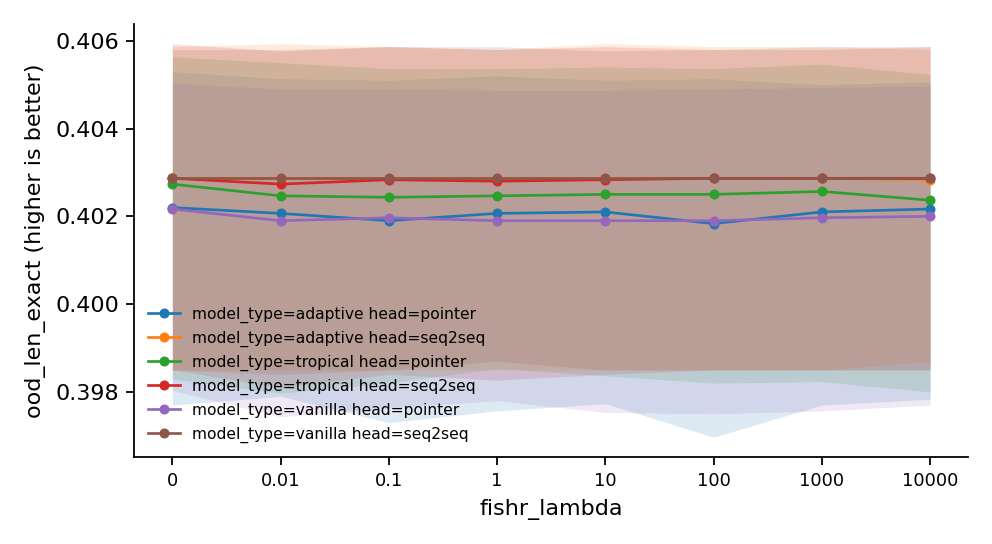
\includegraphics[width=\textwidth]{metric_ood_len_exact.png}
\caption{\texttt{ood\_len\_exact} against \texttt{fishr\_lambda}: the mean over seeds with a 95\% bootstrap CI, one line per combination of the other factors.}
\label{fig:ood_len_exact}
\end{figure}

{\small
\begin{longtable}{lllrlrrr}
\caption{\texttt{ood\_len\_exact} per cell: mean, 95\% bootstrap CI, SD, seeds, diverged runs.}\label{tab:summary-ood_len_exact}\\
\toprule
\texttt{model\_type} & \texttt{head} & \texttt{fishr\_lambda} & mean & 95\% CI & SD & $n$ & div.\\
\midrule
\endhead
adaptive & pointer & 0 & 0.4022 & [0.398, 0.405] & 0.00506 & 5 & 0\\
adaptive & pointer & 0.01 & 0.4021 & [0.398, 0.405] & 0.00499 & 5 & 0\\
adaptive & pointer & 0.1 & 0.4019 & [0.397, 0.405] & 0.00516 & 5 & 0\\
adaptive & pointer & 1 & 0.4021 & [0.398, 0.405] & 0.00509 & 5 & 0\\
adaptive & pointer & 10 & 0.4021 & [0.398, 0.405] & 0.00491 & 5 & 0\\
adaptive & pointer & 100 & 0.4018 & [0.397, 0.405] & 0.00542 & 5 & 0\\
adaptive & pointer & 1000 & 0.4021 & [0.398, 0.405] & 0.00498 & 5 & 0\\
adaptive & pointer & 1e+04 & 0.4022 & [0.398, 0.405] & 0.0049 & 5 & 0\\
adaptive & seq2seq & 0 & 0.4029 & [0.398, 0.406] & 0.00488 & 5 & 0\\
adaptive & seq2seq & 0.01 & 0.4029 & [0.399, 0.406] & 0.00488 & 5 & 0\\
adaptive & seq2seq & 0.1 & 0.4029 & [0.399, 0.406] & 0.00488 & 5 & 0\\
adaptive & seq2seq & 1 & 0.4029 & [0.399, 0.406] & 0.00488 & 5 & 0\\
adaptive & seq2seq & 10 & 0.4029 & [0.399, 0.406] & 0.00488 & 5 & 0\\
adaptive & seq2seq & 100 & 0.4029 & [0.399, 0.406] & 0.00488 & 5 & 0\\
adaptive & seq2seq & 1000 & 0.4029 & [0.399, 0.406] & 0.00488 & 5 & 0\\
adaptive & seq2seq & 1e+04 & 0.4028 & [0.399, 0.406] & 0.00486 & 5 & 0\\
tropical & pointer & 0 & 0.4027 & [0.398, 0.406] & 0.00483 & 5 & 0\\
tropical & pointer & 0.01 & 0.4025 & [0.398, 0.405] & 0.00502 & 5 & 0\\
tropical & pointer & 0.1 & 0.4024 & [0.398, 0.405] & 0.00478 & 5 & 0\\
tropical & pointer & 1 & 0.4025 & [0.399, 0.405] & 0.00485 & 5 & 0\\
tropical & pointer & 10 & 0.4025 & [0.398, 0.405] & 0.00468 & 5 & 0\\
tropical & pointer & 100 & 0.4025 & [0.398, 0.405] & 0.00475 & 5 & 0\\
tropical & pointer & 1000 & 0.4026 & [0.398, 0.405] & 0.00483 & 5 & 0\\
tropical & pointer & 1e+04 & 0.4024 & [0.398, 0.405] & 0.00485 & 5 & 0\\
tropical & seq2seq & 0 & 0.4029 & [0.399, 0.406] & 0.00488 & 5 & 0\\
tropical & seq2seq & 0.01 & 0.4027 & [0.398, 0.406] & 0.00517 & 5 & 0\\
tropical & seq2seq & 0.1 & 0.4028 & [0.398, 0.406] & 0.00496 & 5 & 0\\
tropical & seq2seq & 1 & 0.4028 & [0.398, 0.406] & 0.00493 & 5 & 0\\
tropical & seq2seq & 10 & 0.4028 & [0.398, 0.406] & 0.00496 & 5 & 0\\
tropical & seq2seq & 100 & 0.4029 & [0.399, 0.406] & 0.00488 & 5 & 0\\
tropical & seq2seq & 1000 & 0.4029 & [0.399, 0.406] & 0.00488 & 5 & 0\\
tropical & seq2seq & 1e+04 & 0.4029 & [0.399, 0.406] & 0.00488 & 5 & 0\\
vanilla & pointer & 0 & 0.4022 & [0.398, 0.405] & 0.00466 & 5 & 0\\
vanilla & pointer & 0.01 & 0.4019 & [0.397, 0.405] & 0.00504 & 5 & 0\\
vanilla & pointer & 0.1 & 0.402 & [0.398, 0.405] & 0.00489 & 5 & 0\\
vanilla & pointer & 1 & 0.4019 & [0.398, 0.405] & 0.00488 & 5 & 0\\
vanilla & pointer & 10 & 0.4019 & [0.398, 0.405] & 0.00489 & 5 & 0\\
vanilla & pointer & 100 & 0.4019 & [0.397, 0.405] & 0.00496 & 5 & 0\\
vanilla & pointer & 1000 & 0.402 & [0.398, 0.405] & 0.0049 & 5 & 0\\
vanilla & pointer & 1e+04 & 0.402 & [0.398, 0.405] & 0.00485 & 5 & 0\\
vanilla & seq2seq & 0 & 0.4029 & [0.399, 0.406] & 0.00488 & 5 & 0\\
vanilla & seq2seq & 0.01 & 0.4029 & [0.398, 0.406] & 0.00488 & 5 & 0\\
vanilla & seq2seq & 0.1 & 0.4029 & [0.399, 0.406] & 0.00488 & 5 & 0\\
vanilla & seq2seq & 1 & 0.4029 & [0.399, 0.406] & 0.00488 & 5 & 0\\
vanilla & seq2seq & 10 & 0.4029 & [0.399, 0.406] & 0.00488 & 5 & 0\\
vanilla & seq2seq & 100 & 0.4029 & [0.399, 0.406] & 0.00488 & 5 & 0\\
vanilla & seq2seq & 1000 & 0.4029 & [0.399, 0.406] & 0.00488 & 5 & 0\\
vanilla & seq2seq & 1e+04 & 0.4029 & [0.399, 0.406] & 0.00488 & 5 & 0\\
\bottomrule
\end{longtable}
}

{\small
\begin{longtable}{lllrrrl}
\caption{\texttt{ood\_len\_exact}: each level of \texttt{fishr\_lambda} against its control (0), within each combination of the other factors. parametric: Dunnett vs control.}\label{tab:control-ood_len_exact}\\
\toprule
\texttt{model\_type} & \texttt{head} & \texttt{fishr\_lambda} & difference & 95\% CI & $p$ & \\
\midrule
\endhead
adaptive & pointer & 0.01 & $-1.333\times10^{-4}$ & [-0.00898, 0.00872] & 1.0000 & \\
adaptive & pointer & 0.1 & $-3.000\times10^{-4}$ & [-0.00915, 0.00855] & 1.0000 & \\
adaptive & pointer & 1 & $-1.333\times10^{-4}$ & [-0.00898, 0.00872] & 1.0000 & \\
adaptive & pointer & 10 & $-1.000\times10^{-4}$ & [-0.00895, 0.00875] & 1.0000 & \\
adaptive & pointer & 100 & $-3.667\times10^{-4}$ & [-0.00922, 0.00848] & 1.0000 & \\
adaptive & pointer & 1000 & $-1.000\times10^{-4}$ & [-0.00895, 0.00875] & 1.0000 & \\
adaptive & pointer & 1e+04 & $-3.333\times10^{-5}$ & [-0.00888, 0.00882] & 1.0000 & \\
adaptive & seq2seq & 0.01 & 0 & [-0.00853, 0.00853] & 1.0000 & \\
adaptive & seq2seq & 0.1 & 0 & [-0.00853, 0.00853] & 1.0000 & \\
adaptive & seq2seq & 1 & 0 & [-0.00853, 0.00853] & 1.0000 & \\
adaptive & seq2seq & 10 & 0 & [-0.00853, 0.00853] & 1.0000 & \\
adaptive & seq2seq & 100 & 0 & [-0.00853, 0.00853] & 1.0000 & \\
adaptive & seq2seq & 1000 & 0 & [-0.00853, 0.00853] & 1.0000 & \\
adaptive & seq2seq & 1e+04 & $-3.333\times10^{-5}$ & [-0.00856, 0.00849] & 1.0000 & \\
tropical & pointer & 0.01 & $-2.667\times10^{-4}$ & [-0.00869, 0.00816] & 1.0000 & \\
tropical & pointer & 0.1 & $-3.000\times10^{-4}$ & [-0.00873, 0.00813] & 1.0000 & \\
tropical & pointer & 1 & $-2.667\times10^{-4}$ & [-0.00869, 0.00816] & 1.0000 & \\
tropical & pointer & 10 & $-2.333\times10^{-4}$ & [-0.00866, 0.00819] & 1.0000 & \\
tropical & pointer & 100 & $-2.333\times10^{-4}$ & [-0.00866, 0.00819] & 1.0000 & \\
tropical & pointer & 1000 & $-1.667\times10^{-4}$ & [-0.00859, 0.00826] & 1.0000 & \\
tropical & pointer & 1e+04 & $-3.667\times10^{-4}$ & [-0.00879, 0.00806] & 1.0000 & \\
tropical & seq2seq & 0.01 & $-1.333\times10^{-4}$ & [-0.00877, 0.0085] & 1.0000 & \\
tropical & seq2seq & 0.1 & $-3.333\times10^{-5}$ & [-0.00867, 0.0086] & 1.0000 & \\
tropical & seq2seq & 1 & $-6.667\times10^{-5}$ & [-0.0087, 0.00857] & 1.0000 & \\
tropical & seq2seq & 10 & $-3.333\times10^{-5}$ & [-0.00867, 0.0086] & 1.0000 & \\
tropical & seq2seq & 100 & 0 & [-0.00864, 0.00864] & 1.0000 & \\
tropical & seq2seq & 1000 & 0 & [-0.00864, 0.00864] & 1.0000 & \\
tropical & seq2seq & 1e+04 & 0 & [-0.00864, 0.00864] & 1.0000 & \\
vanilla & pointer & 0.01 & $-2.667\times10^{-4}$ & [-0.0088, 0.00827] & 1.0000 & \\
vanilla & pointer & 0.1 & $-2.000\times10^{-4}$ & [-0.00873, 0.00833] & 1.0000 & \\
vanilla & pointer & 1 & $-2.667\times10^{-4}$ & [-0.0088, 0.00827] & 1.0000 & \\
vanilla & pointer & 10 & $-2.667\times10^{-4}$ & [-0.0088, 0.00827] & 1.0000 & \\
vanilla & pointer & 100 & $-2.667\times10^{-4}$ & [-0.0088, 0.00827] & 1.0000 & \\
vanilla & pointer & 1000 & $-2.000\times10^{-4}$ & [-0.00873, 0.00833] & 1.0000 & \\
vanilla & pointer & 1e+04 & $-1.667\times10^{-4}$ & [-0.0087, 0.00837] & 1.0000 & \\
vanilla & seq2seq & 0.01 & 0 & [-0.00853, 0.00853] & 1.0000 & \\
vanilla & seq2seq & 0.1 & 0 & [-0.00853, 0.00853] & 1.0000 & \\
vanilla & seq2seq & 1 & 0 & [-0.00853, 0.00853] & 1.0000 & \\
vanilla & seq2seq & 10 & 0 & [-0.00853, 0.00853] & 1.0000 & \\
vanilla & seq2seq & 100 & 0 & [-0.00853, 0.00853] & 1.0000 & \\
vanilla & seq2seq & 1000 & 0 & [-0.00853, 0.00853] & 1.0000 & \\
vanilla & seq2seq & 1e+04 & 0 & [-0.00853, 0.00853] & 1.0000 & \\
\bottomrule
\end{longtable}
}

{\small
\begin{longtable}{llrrrrr}
\caption{\texttt{ood\_len\_exact} against log10 \texttt{fishr\_lambda}: parametric: OLS slope t-test, seed-bootstrap CI, with the Jonckheere--Terpstra ordered-trend $\tau$ and $p$.}\label{tab:trend-ood_len_exact}\\
\toprule
\texttt{model\_type} & \texttt{head} & estimate & 95\% CI & $p$ & JT $\tau$ & JT $p$\\
\midrule
\endhead
adaptive & pointer & $1.667\times10^{-5}$ & [$-8.33\times10^{-6}$, $4.88\times10^{-5}$] & 0.9666 & 0.0171 & 0.8996\\
adaptive & seq2seq & $-3.571\times10^{-6}$ & [$-1.07\times10^{-5}$, 0] & 0.9926 & -0.0114 & 0.9300\\
tropical & pointer & $3.965\times10^{-19}$ & [$-2.98\times10^{-5}$, $2.98\times10^{-5}$] & 1.0000 & -0.0133 & 0.9232\\
tropical & seq2seq & $1.905\times10^{-5}$ & [0, $5.48\times10^{-5}$] & 0.9609 & 0.0324 & 0.8164\\
vanilla & pointer & $1.071\times10^{-5}$ & [$-1.07\times10^{-5}$, $3.21\times10^{-5}$] & 0.9778 & 0.0343 & 0.7954\\
vanilla & seq2seq & 0 & [0, 0] & 1.0000 & 0 & 1.0000\\
\bottomrule
\end{longtable}
}

{\small
\begin{longtable}{lrrrl}
\caption{\texttt{ood\_len\_exact}: paired contrasts by seed, Holm-corrected across the cells. parametric: paired t-test by seed, Holm.}\label{tab:paired-ood_len_exact}\\
\toprule
contrast (within) & difference & 95\% CI & $p$ & \\
\midrule
\endhead
\stackcell{model\_type: tropical - vanilla\\\footnotesize head=pointer fishr\_lambda=0 } & $5.667\times10^{-4}$ & [$9.02\times10^{-5}$, 0.00104] & 0.3285 & \\
\stackcell{model\_type: tropical - vanilla\\\footnotesize head=pointer fishr\_lambda=0.01 } & $5.667\times10^{-4}$ & [$-8.12\times10^{-5}$, 0.00121] & 0.6618 & \\
\stackcell{model\_type: tropical - vanilla\\\footnotesize head=pointer fishr\_lambda=0.1 } & $4.667\times10^{-4}$ & [$-1.44\times10^{-4}$, 0.00108] & 0.7073 & \\
\stackcell{model\_type: tropical - vanilla\\\footnotesize head=pointer fishr\_lambda=1 } & $5.667\times10^{-4}$ & [$-2.82\times10^{-4}$, 0.00141] & 0.8233 & \\
\stackcell{model\_type: tropical - vanilla\\\footnotesize head=pointer fishr\_lambda=10 } & $6.000\times10^{-4}$ & [$1.71\times10^{-4}$, 0.00103] & 0.2137 & \\
\stackcell{model\_type: tropical - vanilla\\\footnotesize head=pointer fishr\_lambda=100 } & $6.000\times10^{-4}$ & [$-6.42\times10^{-5}$, 0.00126] & 0.6618 & \\
\stackcell{model\_type: tropical - vanilla\\\footnotesize head=pointer fishr\_lambda=1000 } & $6.000\times10^{-4}$ & [$-6.42\times10^{-5}$, 0.00126] & 0.6618 & \\
\stackcell{model\_type: tropical - vanilla\\\footnotesize head=pointer fishr\_lambda=1e+04 } & $3.667\times10^{-4}$ & [$-3.85\times10^{-4}$, 0.00112] & 0.9887 & \\
\stackcell{model\_type: tropical - vanilla\\\footnotesize head=seq2seq fishr\_lambda=0 } & 0 & [--, --] & -- & \\
\stackcell{model\_type: tropical - vanilla\\\footnotesize head=seq2seq fishr\_lambda=0.01 } & $-1.333\times10^{-4}$ & [$-5.04\times10^{-4}$, $2.37\times10^{-4}$] & 1.0000 & \\
\stackcell{model\_type: tropical - vanilla\\\footnotesize head=seq2seq fishr\_lambda=0.1 } & $-3.333\times10^{-5}$ & [$-1.26\times10^{-4}$, $5.92\times10^{-5}$] & 1.0000 & \\
\stackcell{model\_type: tropical - vanilla\\\footnotesize head=seq2seq fishr\_lambda=1 } & $-6.667\times10^{-5}$ & [$-1.80\times10^{-4}$, $4.67\times10^{-5}$] & 0.8890 & \\
\stackcell{model\_type: tropical - vanilla\\\footnotesize head=seq2seq fishr\_lambda=10 } & $-3.333\times10^{-5}$ & [$-1.26\times10^{-4}$, $5.92\times10^{-5}$] & 1.0000 & \\
\stackcell{model\_type: tropical - vanilla\\\footnotesize head=seq2seq fishr\_lambda=100 } & 0 & [--, --] & -- & \\
\stackcell{model\_type: tropical - vanilla\\\footnotesize head=seq2seq fishr\_lambda=1000 } & 0 & [--, --] & -- & \\
\stackcell{model\_type: tropical - vanilla\\\footnotesize head=seq2seq fishr\_lambda=1e+04 } & 0 & [--, --] & -- & \\
\stackcell{model\_type: adaptive - vanilla\\\footnotesize head=pointer fishr\_lambda=0 } & $3.333\times10^{-5}$ & [$-4.82\times10^{-4}$, $5.49\times10^{-4}$] & 1.0000 & \\
\stackcell{model\_type: adaptive - vanilla\\\footnotesize head=pointer fishr\_lambda=0.01 } & $1.667\times10^{-4}$ & [$-8.68\times10^{-5}$, $4.20\times10^{-4}$] & 0.9935 & \\
\stackcell{model\_type: adaptive - vanilla\\\footnotesize head=pointer fishr\_lambda=0.1 } & $-6.667\times10^{-5}$ & [$-4.96\times10^{-4}$, $3.62\times10^{-4}$] & 1.0000 & \\
\stackcell{model\_type: adaptive - vanilla\\\footnotesize head=pointer fishr\_lambda=1 } & $1.667\times10^{-4}$ & [$-3.19\times10^{-4}$, $6.52\times10^{-4}$] & 1.0000 & \\
\stackcell{model\_type: adaptive - vanilla\\\footnotesize head=pointer fishr\_lambda=10 } & $2.000\times10^{-4}$ & [$2.69\times10^{-5}$, $3.73\times10^{-4}$] & 0.2941 & \\
\stackcell{model\_type: adaptive - vanilla\\\footnotesize head=pointer fishr\_lambda=100 } & $-6.667\times10^{-5}$ & [$-6.45\times10^{-4}$, $5.11\times10^{-4}$] & 1.0000 & \\
\stackcell{model\_type: adaptive - vanilla\\\footnotesize head=pointer fishr\_lambda=1000 } & $1.333\times10^{-4}$ & [$-3.98\times10^{-5}$, $3.06\times10^{-4}$] & 0.7944 & \\
\stackcell{model\_type: adaptive - vanilla\\\footnotesize head=pointer fishr\_lambda=1e+04 } & $1.667\times10^{-4}$ & [$-8.68\times10^{-5}$, $4.20\times10^{-4}$] & 0.9935 & \\
\stackcell{model\_type: adaptive - vanilla\\\footnotesize head=seq2seq fishr\_lambda=0 } & 0 & [--, --] & -- & \\
\stackcell{model\_type: adaptive - vanilla\\\footnotesize head=seq2seq fishr\_lambda=0.01 } & 0 & [--, --] & -- & \\
\stackcell{model\_type: adaptive - vanilla\\\footnotesize head=seq2seq fishr\_lambda=0.1 } & 0 & [--, --] & -- & \\
\stackcell{model\_type: adaptive - vanilla\\\footnotesize head=seq2seq fishr\_lambda=1 } & 0 & [--, --] & -- & \\
\stackcell{model\_type: adaptive - vanilla\\\footnotesize head=seq2seq fishr\_lambda=10 } & 0 & [--, --] & -- & \\
\stackcell{model\_type: adaptive - vanilla\\\footnotesize head=seq2seq fishr\_lambda=100 } & 0 & [--, --] & -- & \\
\stackcell{model\_type: adaptive - vanilla\\\footnotesize head=seq2seq fishr\_lambda=1000 } & 0 & [--, --] & -- & \\
\stackcell{model\_type: adaptive - vanilla\\\footnotesize head=seq2seq fishr\_lambda=1e+04 } & $-3.333\times10^{-5}$ & [$-1.26\times10^{-4}$, $5.92\times10^{-5}$] & 1.0000 & \\
\stackcell{head: pointer - seq2seq\\\footnotesize model\_type=adaptive fishr\_lambda=0 } & $-6.667\times10^{-4}$ & [$-9.59\times10^{-4}$, $-3.74\times10^{-4}$] & 0.0702 & \\
\stackcell{head: pointer - seq2seq\\\footnotesize model\_type=adaptive fishr\_lambda=0.01 } & $-8.000\times10^{-4}$ & [-0.00125, $-3.51\times10^{-4}$] & 0.1241 & \\
\stackcell{head: pointer - seq2seq\\\footnotesize model\_type=adaptive fishr\_lambda=0.1 } & $-9.667\times10^{-4}$ & [-0.00142, $-5.18\times10^{-4}$] & 0.0746 & \\
\stackcell{head: pointer - seq2seq\\\footnotesize model\_type=adaptive fishr\_lambda=1 } & $-8.000\times10^{-4}$ & [-0.00114, $-4.60\times10^{-4}$] & 0.0653 & \\
\stackcell{head: pointer - seq2seq\\\footnotesize model\_type=adaptive fishr\_lambda=10 } & $-7.667\times10^{-4}$ & [-0.00108, $-4.53\times10^{-4}$] & 0.0592 & \\
\stackcell{head: pointer - seq2seq\\\footnotesize model\_type=adaptive fishr\_lambda=100 } & -0.001033 & [-0.00181, $-2.54\times10^{-4}$] & 0.1760 & \\
\stackcell{head: pointer - seq2seq\\\footnotesize model\_type=adaptive fishr\_lambda=1000 } & $-7.667\times10^{-4}$ & [-0.00117, $-3.63\times10^{-4}$] & 0.1051 & \\
\stackcell{head: pointer - seq2seq\\\footnotesize model\_type=adaptive fishr\_lambda=1e+04 } & $-6.667\times10^{-4}$ & [-0.0013, $-2.88\times10^{-5}$] & 0.2287 & \\
\stackcell{head: pointer - seq2seq\\\footnotesize model\_type=tropical fishr\_lambda=0 } & $-1.333\times10^{-4}$ & [$-3.06\times10^{-4}$, $3.98\times10^{-5}$] & 0.2287 & \\
\stackcell{head: pointer - seq2seq\\\footnotesize model\_type=tropical fishr\_lambda=0.01 } & $-2.667\times10^{-4}$ & [$-5.03\times10^{-4}$, $-3.07\times10^{-5}$] & 0.2287 & \\
\stackcell{head: pointer - seq2seq\\\footnotesize model\_type=tropical fishr\_lambda=0.1 } & $-4.000\times10^{-4}$ & [$-7.46\times10^{-4}$, $-5.37\times10^{-5}$] & 0.2287 & \\
\stackcell{head: pointer - seq2seq\\\footnotesize model\_type=tropical fishr\_lambda=1 } & $-3.333\times10^{-4}$ & [$-6.26\times10^{-4}$, $-4.07\times10^{-5}$] & 0.2287 & \\
\stackcell{head: pointer - seq2seq\\\footnotesize model\_type=tropical fishr\_lambda=10 } & $-3.333\times10^{-4}$ & [$-7.20\times10^{-4}$, $5.38\times10^{-5}$] & 0.2287 & \\
\stackcell{head: pointer - seq2seq\\\footnotesize model\_type=tropical fishr\_lambda=100 } & $-3.667\times10^{-4}$ & [$-6.36\times10^{-4}$, $-9.68\times10^{-5}$] & 0.1760 & \\
\stackcell{head: pointer - seq2seq\\\footnotesize model\_type=tropical fishr\_lambda=1000 } & $-3.000\times10^{-4}$ & [$-5.70\times10^{-4}$, $-3.02\times10^{-5}$] & 0.2287 & \\
\stackcell{head: pointer - seq2seq\\\footnotesize model\_type=tropical fishr\_lambda=1e+04 } & $-5.000\times10^{-4}$ & [$-8.27\times10^{-4}$, $-1.73\times10^{-4}$] & 0.1324 & \\
\stackcell{head: pointer - seq2seq\\\footnotesize model\_type=vanilla fishr\_lambda=0 } & $-7.000\times10^{-4}$ & [-0.0011, $-3.02\times10^{-4}$] & 0.1241 & \\
\stackcell{head: pointer - seq2seq\\\footnotesize model\_type=vanilla fishr\_lambda=0.01 } & $-9.667\times10^{-4}$ & [-0.00156, $-3.74\times10^{-4}$] & 0.1241 & \\
\stackcell{head: pointer - seq2seq\\\footnotesize model\_type=vanilla fishr\_lambda=0.1 } & $-9.000\times10^{-4}$ & [-0.00144, $-3.60\times10^{-4}$] & 0.1241 & \\
\stackcell{head: pointer - seq2seq\\\footnotesize model\_type=vanilla fishr\_lambda=1 } & $-9.667\times10^{-4}$ & [-0.00152, $-4.11\times10^{-4}$] & 0.1241 & \\
\stackcell{head: pointer - seq2seq\\\footnotesize model\_type=vanilla fishr\_lambda=10 } & $-9.667\times10^{-4}$ & [-0.00139, $-5.43\times10^{-4}$] & 0.0702 & \\
\stackcell{head: pointer - seq2seq\\\footnotesize model\_type=vanilla fishr\_lambda=100 } & $-9.667\times10^{-4}$ & [-0.00146, $-4.73\times10^{-4}$] & 0.1003 & \\
\stackcell{head: pointer - seq2seq\\\footnotesize model\_type=vanilla fishr\_lambda=1000 } & $-9.000\times10^{-4}$ & [-0.0013, $-4.97\times10^{-4}$] & 0.0702 & \\
\stackcell{head: pointer - seq2seq\\\footnotesize model\_type=vanilla fishr\_lambda=1e+04 } & $-8.667\times10^{-4}$ & [-0.00138, $-3.51\times10^{-4}$] & 0.1241 & \\
\bottomrule
\end{longtable}
}

\subsection{\texttt{ood\_val\_f1}}
\begin{figure}[tbp]
\centering
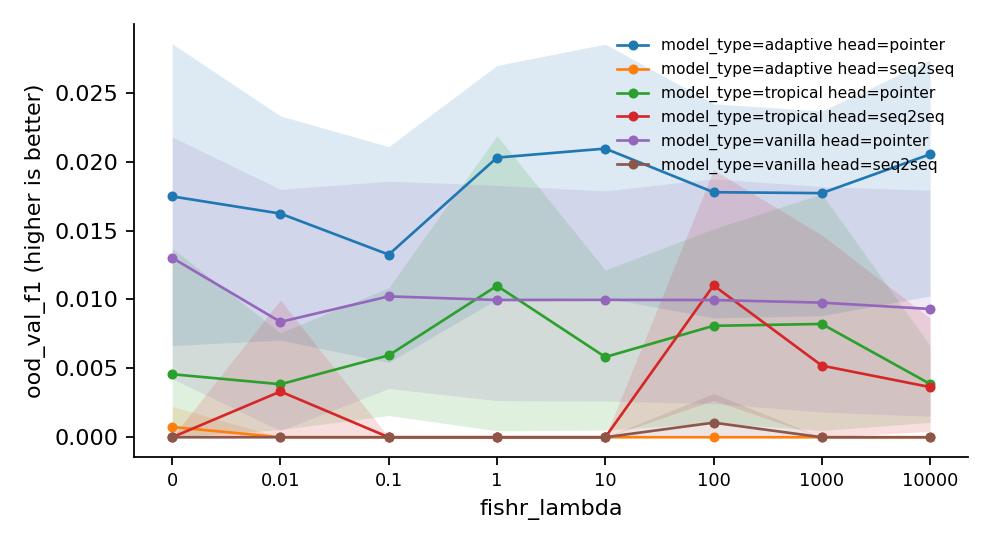
\includegraphics[width=\textwidth]{metric_ood_val_f1.png}
\caption{\texttt{ood\_val\_f1} against \texttt{fishr\_lambda}: the mean over seeds with a 95\% bootstrap CI, one line per combination of the other factors.}
\label{fig:ood_val_f1}
\end{figure}

{\small
\begin{longtable}{lllrlrrr}
\caption{\texttt{ood\_val\_f1} per cell: mean, 95\% bootstrap CI, SD, seeds, diverged runs.}\label{tab:summary-ood_val_f1}\\
\toprule
\texttt{model\_type} & \texttt{head} & \texttt{fishr\_lambda} & mean & 95\% CI & SD & $n$ & div.\\
\midrule
\endhead
adaptive & pointer & 0 & 0.01748 & [0.00665, 0.0286] & 0.0134 & 5 & 0\\
adaptive & pointer & 0.01 & 0.01623 & [0.00705, 0.0233] & 0.0104 & 5 & 0\\
adaptive & pointer & 0.1 & 0.01326 & [0.00542, 0.0211] & 0.0103 & 5 & 0\\
adaptive & pointer & 1 & 0.0203 & [0.01, 0.027] & 0.0116 & 5 & 0\\
adaptive & pointer & 10 & 0.02095 & [0.0101, 0.0285] & 0.0122 & 5 & 0\\
adaptive & pointer & 100 & 0.01778 & [0.00866, 0.0242] & 0.0104 & 5 & 0\\
adaptive & pointer & 1000 & 0.01772 & [0.00882, 0.0237] & 0.0102 & 5 & 0\\
adaptive & pointer & 1e+04 & 0.02054 & [0.0103, 0.0274] & 0.0118 & 5 & 0\\
adaptive & seq2seq & 0 & $7.477\times10^{-4}$ & [0, 0.00224] & 0.00167 & 5 & 0\\
adaptive & seq2seq & 0.01 & 0 & [0, 0] & 0 & 5 & 0\\
adaptive & seq2seq & 0.1 & 0 & [0, 0] & 0 & 5 & 0\\
adaptive & seq2seq & 1 & 0 & [0, 0] & 0 & 5 & 0\\
adaptive & seq2seq & 10 & 0 & [0, 0] & 0 & 5 & 0\\
adaptive & seq2seq & 100 & 0 & [0, 0] & 0 & 5 & 0\\
adaptive & seq2seq & 1000 & 0 & [0, 0] & 0 & 5 & 0\\
adaptive & seq2seq & 1e+04 & 0 & [0, 0] & 0 & 5 & 0\\
tropical & pointer & 0 & 0.004575 & [0, 0.0137] & 0.0102 & 5 & 0\\
tropical & pointer & 0.01 & 0.003848 & [$5.57\times10^{-4}$, 0.00758] & 0.00425 & 5 & 0\\
tropical & pointer & 0.1 & 0.005947 & [0.00158, 0.0109] & 0.00613 & 5 & 0\\
tropical & pointer & 1 & 0.01099 & [$4.71\times10^{-4}$, 0.0219] & 0.0141 & 5 & 0\\
tropical & pointer & 10 & 0.005823 & [$5.19\times10^{-4}$, 0.0121] & 0.00739 & 5 & 0\\
tropical & pointer & 100 & 0.008088 & [0.00105, 0.0151] & 0.00897 & 5 & 0\\
tropical & pointer & 1000 & 0.008224 & [$4.91\times10^{-4}$, 0.0177] & 0.0118 & 5 & 0\\
tropical & pointer & 1e+04 & 0.003867 & [0.00108, 0.00665] & 0.00362 & 5 & 0\\
tropical & seq2seq & 0 & 0 & [0, 0] & 0 & 5 & 0\\
tropical & seq2seq & 0.01 & 0.003322 & [0, 0.00997] & 0.00743 & 5 & 0\\
tropical & seq2seq & 0.1 & 0 & [0, 0] & 0 & 5 & 0\\
tropical & seq2seq & 1 & 0 & [0, 0] & 0 & 5 & 0\\
tropical & seq2seq & 10 & 0 & [0, 0] & 0 & 5 & 0\\
tropical & seq2seq & 100 & 0.01102 & [0.00268, 0.0194] & 0.0116 & 5 & 0\\
tropical & seq2seq & 1000 & 0.005198 & [0, 0.0147] & 0.0104 & 5 & 0\\
tropical & seq2seq & 1e+04 & 0.003642 & [$4.24\times10^{-4}$, 0.00865] & 0.00568 & 5 & 0\\
vanilla & pointer & 0 & 0.01302 & [0.00425, 0.0218] & 0.0111 & 5 & 0\\
vanilla & pointer & 0.01 & 0.008373 & [$4.86\times10^{-4}$, 0.018] & 0.0111 & 5 & 0\\
vanilla & pointer & 0.1 & 0.01023 & [0.00354, 0.0186] & 0.00962 & 5 & 0\\
vanilla & pointer & 1 & 0.009962 & [0.00266, 0.0183] & 0.01 & 5 & 0\\
vanilla & pointer & 10 & 0.009972 & [0.00263, 0.0179] & 0.0101 & 5 & 0\\
vanilla & pointer & 100 & 0.00996 & [0.00246, 0.0188] & 0.0104 & 5 & 0\\
vanilla & pointer & 1000 & 0.00977 & [0.00183, 0.0182] & 0.0107 & 5 & 0\\
vanilla & pointer & 1e+04 & 0.009312 & [0.00153, 0.0179] & 0.0106 & 5 & 0\\
vanilla & seq2seq & 0 & 0 & [0, 0] & 0 & 5 & 0\\
vanilla & seq2seq & 0.01 & 0 & [0, 0] & 0 & 5 & 0\\
vanilla & seq2seq & 0.1 & 0 & [0, 0] & 0 & 5 & 0\\
vanilla & seq2seq & 1 & 0 & [0, 0] & 0 & 5 & 0\\
vanilla & seq2seq & 10 & 0 & [0, 0] & 0 & 5 & 0\\
vanilla & seq2seq & 100 & 0.001058 & [0, 0.00317] & 0.00237 & 5 & 0\\
vanilla & seq2seq & 1000 & 0 & [0, 0] & 0 & 5 & 0\\
vanilla & seq2seq & 1e+04 & 0 & [0, 0] & 0 & 5 & 0\\
\bottomrule
\end{longtable}
}

{\small
\begin{longtable}{lllrrrl}
\caption{\texttt{ood\_val\_f1}: each level of \texttt{fishr\_lambda} against its control (0), within each combination of the other factors. rank: Wilcoxon signed-rank by seed, Holm.}\label{tab:control-ood_val_f1}\\
\toprule
\texttt{model\_type} & \texttt{head} & \texttt{fishr\_lambda} & difference & 95\% CI & $p$ & \\
\midrule
\endhead
adaptive & pointer & 0.01 & $1.438\times10^{-5}$ & [-0.00882, 0.00479] & 1.0000 & \\
adaptive & pointer & 0.1 & -0.001521 & [-0.0136, 0.00342] & 1.0000 & \\
adaptive & pointer & 1 & $7.829\times10^{-4}$ & [-0.00521, 0.0111] & 1.0000 & \\
adaptive & pointer & 10 & $4.566\times10^{-4}$ & [-0.00474, 0.0125] & 1.0000 & \\
adaptive & pointer & 100 & $4.635\times10^{-5}$ & [-0.0063, 0.00602] & 1.0000 & \\
adaptive & pointer & 1000 & 0 & [-0.00665, 0.006] & 1.0000 & \\
adaptive & pointer & 1e+04 & $1.553\times10^{-4}$ & [-0.00473, 0.0117] & 1.0000 & \\
adaptive & seq2seq & 0.01 & 0 & [-0.00224, 0] & 1.0000 & \\
adaptive & seq2seq & 0.1 & 0 & [-0.00224, 0] & 1.0000 & \\
adaptive & seq2seq & 1 & 0 & [-0.00224, 0] & 1.0000 & \\
adaptive & seq2seq & 10 & 0 & [-0.00224, 0] & 1.0000 & \\
adaptive & seq2seq & 100 & 0 & [-0.00224, 0] & 1.0000 & \\
adaptive & seq2seq & 1000 & 0 & [-0.00224, 0] & 1.0000 & \\
adaptive & seq2seq & 1e+04 & 0 & [-0.00224, 0] & 1.0000 & \\
tropical & pointer & 0.01 & 0 & [-0.00748, 0.00419] & 1.0000 & \\
tropical & pointer & 0.1 & 0.002561 & [-0.00374, 0.006] & 1.0000 & \\
tropical & pointer & 1 & 0.001329 & [$2.66\times10^{-4}$, 0.0175] & 1.0000 & \\
tropical & pointer & 10 & 0 & [-0.00755, 0.0103] & 1.0000 & \\
tropical & pointer & 100 & 0 & [-0.00175, 0.01] & 1.0000 & \\
tropical & pointer & 1000 & 0.002457 & [$4.91\times10^{-4}$, 0.00751] & 1.0000 & \\
tropical & pointer & 1e+04 & 0 & [-0.0089, 0.00569] & 1.0000 & \\
tropical & seq2seq & 0.01 & 0 & [0, 0.00997] & 1.0000 & \\
tropical & seq2seq & 0.1 & 0 & [0, 0] & -- & \\
tropical & seq2seq & 1 & 0 & [0, 0] & -- & \\
tropical & seq2seq & 10 & 0 & [0, 0] & -- & \\
tropical & seq2seq & 100 & 0.01338 & [0.00268, 0.0194] & 1.0000 & \\
tropical & seq2seq & 1000 & 0 & [0, 0.0147] & 1.0000 & \\
tropical & seq2seq & 1e+04 & 0.002121 & [$4.24\times10^{-4}$, 0.00865] & 1.0000 & \\
vanilla & pointer & 0.01 & -0.001074 & [-0.0139, 0.00113] & 1.0000 & \\
vanilla & pointer & 0.1 & $-4.475\times10^{-6}$ & [-0.00958, 0.00135] & 1.0000 & \\
vanilla & pointer & 1 & -0.001341 & [-0.0089, $9.78\times10^{-4}$] & 1.0000 & \\
vanilla & pointer & 10 & -0.001251 & [-0.00896, 0.00103] & 1.0000 & \\
vanilla & pointer & 100 & -0.001327 & [-0.00932, 0.00135] & 1.0000 & \\
vanilla & pointer & 1000 & -0.001174 & [-0.00837, $2.82\times10^{-4}$] & 1.0000 & \\
vanilla & pointer & 1e+04 & -0.001678 & [-0.00933, $7.23\times10^{-5}$] & 1.0000 & \\
vanilla & seq2seq & 0.01 & 0 & [0, 0] & -- & \\
vanilla & seq2seq & 0.1 & 0 & [0, 0] & -- & \\
vanilla & seq2seq & 1 & 0 & [0, 0] & -- & \\
vanilla & seq2seq & 10 & 0 & [0, 0] & -- & \\
vanilla & seq2seq & 100 & 0 & [0, 0.00317] & 1.0000 & \\
vanilla & seq2seq & 1000 & 0 & [0, 0] & -- & \\
vanilla & seq2seq & 1e+04 & 0 & [0, 0] & -- & \\
\bottomrule
\end{longtable}
}

{\small
\begin{longtable}{llrrrrr}
\caption{\texttt{ood\_val\_f1} against log10 \texttt{fishr\_lambda}: rank: Spearman rho, seed-bootstrap CI, with the Jonckheere--Terpstra ordered-trend $\tau$ and $p$.}\label{tab:trend-ood_val_f1}\\
\toprule
\texttt{model\_type} & \texttt{head} & estimate & 95\% CI & $p$ & JT $\tau$ & JT $p$\\
\midrule
\endhead
adaptive & pointer & 0.1505 & [-0.0855, 0.411] & 0.3881 & 0.11 & 0.4037\\
adaptive & seq2seq & -- & [--, --] & -- & -- & --\\
tropical & pointer & -0.02251 & [-0.367, 0.36] & 0.8979 & -0.019 & 0.8872\\
tropical & seq2seq & 0.382 & [0.177, 0.613] & 0.0235 & 0.219 & 0.0324\\
vanilla & pointer & -0.02425 & [-0.386, 0.282] & 0.8900 & -0.0248 & 0.8476\\
vanilla & seq2seq & 0.08575 & [0.0857, 0.153] & 0.6243 & 0.019 & 0.8516\\
\bottomrule
\end{longtable}
}

{\small
\begin{longtable}{lrrrl}
\caption{\texttt{ood\_val\_f1}: paired contrasts by seed, Holm-corrected across the cells. rank: Wilcoxon signed-rank by seed, Holm.}\label{tab:paired-ood_val_f1}\\
\toprule
contrast (within) & difference & 95\% CI & $p$ & \\
\midrule
\endhead
\stackcell{model\_type: tropical - vanilla\\\footnotesize head=pointer fishr\_lambda=0 } & -0.008446 & [-0.0261, 0.00923] & 1.0000 & \\
\stackcell{model\_type: tropical - vanilla\\\footnotesize head=pointer fishr\_lambda=0.01 } & -0.004525 & [-0.0198, 0.0108] & 1.0000 & \\
\stackcell{model\_type: tropical - vanilla\\\footnotesize head=pointer fishr\_lambda=0.1 } & -0.004279 & [-0.0182, 0.00968] & 1.0000 & \\
\stackcell{model\_type: tropical - vanilla\\\footnotesize head=pointer fishr\_lambda=1 } & 0.001031 & [-0.023, 0.0251] & 1.0000 & \\
\stackcell{model\_type: tropical - vanilla\\\footnotesize head=pointer fishr\_lambda=10 } & -0.004149 & [-0.0231, 0.0148] & 1.0000 & \\
\stackcell{model\_type: tropical - vanilla\\\footnotesize head=pointer fishr\_lambda=100 } & -0.001871 & [-0.0102, 0.00643] & 1.0000 & \\
\stackcell{model\_type: tropical - vanilla\\\footnotesize head=pointer fishr\_lambda=1000 } & -0.001546 & [-0.0152, 0.0121] & 1.0000 & \\
\stackcell{model\_type: tropical - vanilla\\\footnotesize head=pointer fishr\_lambda=1e+04 } & -0.005445 & [-0.0163, 0.00541] & 1.0000 & \\
\stackcell{model\_type: tropical - vanilla\\\footnotesize head=seq2seq fishr\_lambda=0 } & 0 & [--, --] & -- & \\
\stackcell{model\_type: tropical - vanilla\\\footnotesize head=seq2seq fishr\_lambda=0.01 } & 0.003322 & [-0.0059, 0.0125] & 1.0000 & \\
\stackcell{model\_type: tropical - vanilla\\\footnotesize head=seq2seq fishr\_lambda=0.1 } & 0 & [--, --] & -- & \\
\stackcell{model\_type: tropical - vanilla\\\footnotesize head=seq2seq fishr\_lambda=1 } & 0 & [--, --] & -- & \\
\stackcell{model\_type: tropical - vanilla\\\footnotesize head=seq2seq fishr\_lambda=10 } & 0 & [--, --] & -- & \\
\stackcell{model\_type: tropical - vanilla\\\footnotesize head=seq2seq fishr\_lambda=100 } & 0.009963 & [-0.00426, 0.0242] & 1.0000 & \\
\stackcell{model\_type: tropical - vanilla\\\footnotesize head=seq2seq fishr\_lambda=1000 } & 0.005198 & [-0.0077, 0.0181] & 1.0000 & \\
\stackcell{model\_type: tropical - vanilla\\\footnotesize head=seq2seq fishr\_lambda=1e+04 } & 0.003642 & [-0.00341, 0.0107] & 1.0000 & \\
\stackcell{model\_type: adaptive - vanilla\\\footnotesize head=pointer fishr\_lambda=0 } & 0.00446 & [-0.015, 0.024] & 1.0000 & \\
\stackcell{model\_type: adaptive - vanilla\\\footnotesize head=pointer fishr\_lambda=0.01 } & 0.007861 & [-0.00246, 0.0182] & 1.0000 & \\
\stackcell{model\_type: adaptive - vanilla\\\footnotesize head=pointer fishr\_lambda=0.1 } & 0.003031 & [-0.00717, 0.0132] & 1.0000 & \\
\stackcell{model\_type: adaptive - vanilla\\\footnotesize head=pointer fishr\_lambda=1 } & 0.01033 & [-0.00246, 0.0231] & 1.0000 & \\
\stackcell{model\_type: adaptive - vanilla\\\footnotesize head=pointer fishr\_lambda=10 } & 0.01098 & [-0.00239, 0.0243] & 1.0000 & \\
\stackcell{model\_type: adaptive - vanilla\\\footnotesize head=pointer fishr\_lambda=100 } & 0.007824 & [-0.00231, 0.018] & 1.0000 & \\
\stackcell{model\_type: adaptive - vanilla\\\footnotesize head=pointer fishr\_lambda=1000 } & 0.007948 & [-0.00303, 0.0189] & 1.0000 & \\
\stackcell{model\_type: adaptive - vanilla\\\footnotesize head=pointer fishr\_lambda=1e+04 } & 0.01123 & [-0.00246, 0.0249] & 1.0000 & \\
\stackcell{model\_type: adaptive - vanilla\\\footnotesize head=seq2seq fishr\_lambda=0 } & $7.477\times10^{-4}$ & [-0.00133, 0.00282] & 1.0000 & \\
\stackcell{model\_type: adaptive - vanilla\\\footnotesize head=seq2seq fishr\_lambda=0.01 } & 0 & [--, --] & -- & \\
\stackcell{model\_type: adaptive - vanilla\\\footnotesize head=seq2seq fishr\_lambda=0.1 } & 0 & [--, --] & -- & \\
\stackcell{model\_type: adaptive - vanilla\\\footnotesize head=seq2seq fishr\_lambda=1 } & 0 & [--, --] & -- & \\
\stackcell{model\_type: adaptive - vanilla\\\footnotesize head=seq2seq fishr\_lambda=10 } & 0 & [--, --] & -- & \\
\stackcell{model\_type: adaptive - vanilla\\\footnotesize head=seq2seq fishr\_lambda=100 } & -0.001058 & [-0.004, 0.00188] & 1.0000 & \\
\stackcell{model\_type: adaptive - vanilla\\\footnotesize head=seq2seq fishr\_lambda=1000 } & 0 & [--, --] & -- & \\
\stackcell{model\_type: adaptive - vanilla\\\footnotesize head=seq2seq fishr\_lambda=1e+04 } & 0 & [--, --] & -- & \\
\stackcell{head: pointer - seq2seq\\\footnotesize model\_type=adaptive fishr\_lambda=0 } & 0.01673 & [-0.00147, 0.0349] & 1.0000 & \\
\stackcell{head: pointer - seq2seq\\\footnotesize model\_type=adaptive fishr\_lambda=0.01 } & 0.01623 & [0.00327, 0.0292] & 1.0000 & \\
\stackcell{head: pointer - seq2seq\\\footnotesize model\_type=adaptive fishr\_lambda=0.1 } & 0.01326 & [$5.09\times10^{-4}$, 0.026] & 1.0000 & \\
\stackcell{head: pointer - seq2seq\\\footnotesize model\_type=adaptive fishr\_lambda=1 } & 0.0203 & [0.00588, 0.0347] & 1.0000 & \\
\stackcell{head: pointer - seq2seq\\\footnotesize model\_type=adaptive fishr\_lambda=10 } & 0.02095 & [0.00579, 0.0361] & 1.0000 & \\
\stackcell{head: pointer - seq2seq\\\footnotesize model\_type=adaptive fishr\_lambda=100 } & 0.01778 & [0.00488, 0.0307] & 1.0000 & \\
\stackcell{head: pointer - seq2seq\\\footnotesize model\_type=adaptive fishr\_lambda=1000 } & 0.01772 & [0.00505, 0.0304] & 1.0000 & \\
\stackcell{head: pointer - seq2seq\\\footnotesize model\_type=adaptive fishr\_lambda=1e+04 } & 0.02054 & [0.00584, 0.0352] & 1.0000 & \\
\stackcell{head: pointer - seq2seq\\\footnotesize model\_type=tropical fishr\_lambda=0 } & 0.004575 & [-0.00813, 0.0173] & 1.0000 & \\
\stackcell{head: pointer - seq2seq\\\footnotesize model\_type=tropical fishr\_lambda=0.01 } & $5.264\times10^{-4}$ & [-0.0122, 0.0133] & 1.0000 & \\
\stackcell{head: pointer - seq2seq\\\footnotesize model\_type=tropical fishr\_lambda=0.1 } & 0.005947 & [-0.00166, 0.0136] & 1.0000 & \\
\stackcell{head: pointer - seq2seq\\\footnotesize model\_type=tropical fishr\_lambda=1 } & 0.01099 & [-0.0065, 0.0285] & 1.0000 & \\
\stackcell{head: pointer - seq2seq\\\footnotesize model\_type=tropical fishr\_lambda=10 } & 0.005823 & [-0.00335, 0.015] & 1.0000 & \\
\stackcell{head: pointer - seq2seq\\\footnotesize model\_type=tropical fishr\_lambda=100 } & -0.002933 & [-0.0278, 0.0219] & 1.0000 & \\
\stackcell{head: pointer - seq2seq\\\footnotesize model\_type=tropical fishr\_lambda=1000 } & 0.003026 & [-0.0203, 0.0263] & 1.0000 & \\
\stackcell{head: pointer - seq2seq\\\footnotesize model\_type=tropical fishr\_lambda=1e+04 } & $2.249\times10^{-4}$ & [-0.00745, 0.0079] & 1.0000 & \\
\stackcell{head: pointer - seq2seq\\\footnotesize model\_type=vanilla fishr\_lambda=0 } & 0.01302 & [$-7.71\times10^{-4}$, 0.0268] & 1.0000 & \\
\stackcell{head: pointer - seq2seq\\\footnotesize model\_type=vanilla fishr\_lambda=0.01 } & 0.008373 & [-0.00543, 0.0222] & 1.0000 & \\
\stackcell{head: pointer - seq2seq\\\footnotesize model\_type=vanilla fishr\_lambda=0.1 } & 0.01023 & [-0.00172, 0.0222] & 1.0000 & \\
\stackcell{head: pointer - seq2seq\\\footnotesize model\_type=vanilla fishr\_lambda=1 } & 0.009962 & [-0.00247, 0.0224] & 1.0000 & \\
\stackcell{head: pointer - seq2seq\\\footnotesize model\_type=vanilla fishr\_lambda=10 } & 0.009972 & [-0.00253, 0.0225] & 1.0000 & \\
\stackcell{head: pointer - seq2seq\\\footnotesize model\_type=vanilla fishr\_lambda=100 } & 0.008901 & [-0.00584, 0.0236] & 1.0000 & \\
\stackcell{head: pointer - seq2seq\\\footnotesize model\_type=vanilla fishr\_lambda=1000 } & 0.00977 & [-0.00356, 0.0231] & 1.0000 & \\
\stackcell{head: pointer - seq2seq\\\footnotesize model\_type=vanilla fishr\_lambda=1e+04 } & 0.009312 & [-0.00388, 0.0225] & 1.0000 & \\
\bottomrule
\end{longtable}
}

\subsection{\texttt{ood\_val\_exact}}
\begin{figure}[tbp]
\centering
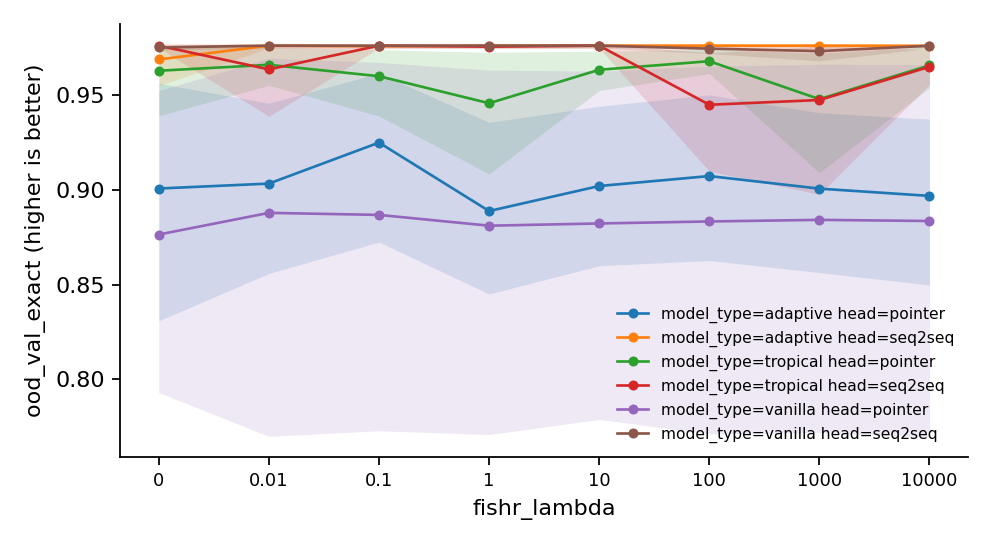
\includegraphics[width=\textwidth]{metric_ood_val_exact.png}
\caption{\texttt{ood\_val\_exact} against \texttt{fishr\_lambda}: the mean over seeds with a 95\% bootstrap CI, one line per combination of the other factors.}
\label{fig:ood_val_exact}
\end{figure}

{\small
\begin{longtable}{lllrlrrr}
\caption{\texttt{ood\_val\_exact} per cell: mean, 95\% bootstrap CI, SD, seeds, diverged runs.}\label{tab:summary-ood_val_exact}\\
\toprule
\texttt{model\_type} & \texttt{head} & \texttt{fishr\_lambda} & mean & 95\% CI & SD & $n$ & div.\\
\midrule
\endhead
adaptive & pointer & 0 & 0.9007 & [0.831, 0.956] & 0.0827 & 5 & 0\\
adaptive & pointer & 0.01 & 0.9033 & [0.856, 0.946] & 0.0561 & 5 & 0\\
adaptive & pointer & 0.1 & 0.925 & [0.872, 0.962] & 0.0598 & 5 & 0\\
adaptive & pointer & 1 & 0.8888 & [0.845, 0.936] & 0.0589 & 5 & 0\\
adaptive & pointer & 10 & 0.902 & [0.86, 0.944] & 0.0583 & 5 & 0\\
adaptive & pointer & 100 & 0.9073 & [0.863, 0.95] & 0.0566 & 5 & 0\\
adaptive & pointer & 1000 & 0.9006 & [0.856, 0.941] & 0.0533 & 5 & 0\\
adaptive & pointer & 1e+04 & 0.8968 & [0.85, 0.937] & 0.056 & 5 & 0\\
adaptive & seq2seq & 0 & 0.9689 & [0.955, 0.976] & 0.0154 & 5 & 0\\
adaptive & seq2seq & 0.01 & 0.9762 & [0.975, 0.977] & 0.00141 & 5 & 0\\
adaptive & seq2seq & 0.1 & 0.9759 & [0.975, 0.976] & 0.00111 & 5 & 0\\
adaptive & seq2seq & 1 & 0.9762 & [0.975, 0.977] & 0.00141 & 5 & 0\\
adaptive & seq2seq & 10 & 0.9762 & [0.975, 0.977] & 0.00141 & 5 & 0\\
adaptive & seq2seq & 100 & 0.9762 & [0.975, 0.977] & 0.00141 & 5 & 0\\
adaptive & seq2seq & 1000 & 0.9762 & [0.975, 0.977] & 0.00141 & 5 & 0\\
adaptive & seq2seq & 1e+04 & 0.9761 & [0.975, 0.977] & 0.00132 & 5 & 0\\
tropical & pointer & 0 & 0.9629 & [0.939, 0.976] & 0.0265 & 5 & 0\\
tropical & pointer & 0.01 & 0.966 & [0.955, 0.975] & 0.0126 & 5 & 0\\
tropical & pointer & 0.1 & 0.96 & [0.939, 0.974] & 0.0234 & 5 & 0\\
tropical & pointer & 1 & 0.9457 & [0.908, 0.973] & 0.0418 & 5 & 0\\
tropical & pointer & 10 & 0.9634 & [0.952, 0.973] & 0.0132 & 5 & 0\\
tropical & pointer & 100 & 0.9679 & [0.961, 0.974] & 0.00825 & 5 & 0\\
tropical & pointer & 1000 & 0.9479 & [0.909, 0.972] & 0.0436 & 5 & 0\\
tropical & pointer & 1e+04 & 0.9657 & [0.954, 0.976] & 0.0139 & 5 & 0\\
tropical & seq2seq & 0 & 0.9762 & [0.975, 0.977] & 0.00141 & 5 & 0\\
tropical & seq2seq & 0.01 & 0.9636 & [0.939, 0.977] & 0.0277 & 5 & 0\\
tropical & seq2seq & 0.1 & 0.9762 & [0.975, 0.977] & 0.00141 & 5 & 0\\
tropical & seq2seq & 1 & 0.9756 & [0.975, 0.976] & 0.00104 & 5 & 0\\
tropical & seq2seq & 10 & 0.9761 & [0.975, 0.977] & 0.00138 & 5 & 0\\
tropical & seq2seq & 100 & 0.9449 & [0.91, 0.972] & 0.0402 & 5 & 0\\
tropical & seq2seq & 1000 & 0.9474 & [0.898, 0.976] & 0.0546 & 5 & 0\\
tropical & seq2seq & 1e+04 & 0.965 & [0.956, 0.974] & 0.0116 & 5 & 0\\
vanilla & pointer & 0 & 0.8764 & [0.793, 0.952] & 0.109 & 5 & 0\\
vanilla & pointer & 0.01 & 0.8878 & [0.77, 0.969] & 0.131 & 5 & 0\\
vanilla & pointer & 0.1 & 0.8868 & [0.773, 0.967] & 0.127 & 5 & 0\\
vanilla & pointer & 1 & 0.8811 & [0.771, 0.963] & 0.126 & 5 & 0\\
vanilla & pointer & 10 & 0.8822 & [0.779, 0.963] & 0.122 & 5 & 0\\
vanilla & pointer & 100 & 0.8833 & [0.771, 0.965] & 0.126 & 5 & 0\\
vanilla & pointer & 1000 & 0.8841 & [0.772, 0.966] & 0.126 & 5 & 0\\
vanilla & pointer & 1e+04 & 0.8835 & [0.769, 0.966] & 0.128 & 5 & 0\\
vanilla & seq2seq & 0 & 0.9752 & [0.974, 0.976] & 0.00163 & 5 & 0\\
vanilla & seq2seq & 0.01 & 0.9762 & [0.975, 0.977] & 0.00141 & 5 & 0\\
vanilla & seq2seq & 0.1 & 0.9761 & [0.975, 0.977] & 0.00141 & 5 & 0\\
vanilla & seq2seq & 1 & 0.9762 & [0.975, 0.977] & 0.00141 & 5 & 0\\
vanilla & seq2seq & 10 & 0.9762 & [0.975, 0.977] & 0.00141 & 5 & 0\\
vanilla & seq2seq & 100 & 0.9746 & [0.972, 0.976] & 0.00283 & 5 & 0\\
vanilla & seq2seq & 1000 & 0.9733 & [0.968, 0.976] & 0.00563 & 5 & 0\\
vanilla & seq2seq & 1e+04 & 0.9761 & [0.975, 0.977] & 0.00135 & 5 & 0\\
\bottomrule
\end{longtable}
}

{\small
\begin{longtable}{lllrrrl}
\caption{\texttt{ood\_val\_exact}: each level of \texttt{fishr\_lambda} against its control (0), within each combination of the other factors. parametric: Dunnett vs control.}\label{tab:control-ood_val_exact}\\
\toprule
\texttt{model\_type} & \texttt{head} & \texttt{fishr\_lambda} & difference & 95\% CI & $p$ & \\
\midrule
\endhead
adaptive & pointer & 0.01 & 0.0026 & [-0.104, 0.109] & 1.0000 & \\
adaptive & pointer & 0.1 & 0.02426 & [-0.082, 0.131] & 0.9828 & \\
adaptive & pointer & 1 & -0.0119 & [-0.118, 0.0944] & 0.9998 & \\
adaptive & pointer & 10 & 0.00132 & [-0.105, 0.108] & 1.0000 & \\
adaptive & pointer & 100 & 0.00658 & [-0.0997, 0.113] & 1.0000 & \\
adaptive & pointer & 1000 & $-6.000\times10^{-5}$ & [-0.106, 0.106] & 1.0000 & \\
adaptive & pointer & 1e+04 & -0.0039 & [-0.11, 0.102] & 1.0000 & \\
adaptive & seq2seq & 0.01 & 0.00728 & [-0.00249, 0.017] & 0.2135 & \\
adaptive & seq2seq & 0.1 & 0.007 & [-0.00277, 0.0168] & 0.2459 & \\
adaptive & seq2seq & 1 & 0.00728 & [-0.00249, 0.017] & 0.2135 & \\
adaptive & seq2seq & 10 & 0.00728 & [-0.00249, 0.017] & 0.2135 & \\
adaptive & seq2seq & 100 & 0.00728 & [-0.00249, 0.017] & 0.2136 & \\
adaptive & seq2seq & 1000 & 0.00728 & [-0.00249, 0.017] & 0.2134 & \\
adaptive & seq2seq & 1e+04 & 0.00718 & [-0.00259, 0.0169] & 0.2246 & \\
tropical & pointer & 0.01 & 0.00314 & [-0.0427, 0.0489] & 1.0000 & \\
tropical & pointer & 0.1 & -0.00288 & [-0.0487, 0.0429] & 1.0000 & \\
tropical & pointer & 1 & -0.01716 & [-0.063, 0.0286] & 0.8347 & \\
tropical & pointer & 10 & $5.200\times10^{-4}$ & [-0.0453, 0.0463] & 1.0000 & \\
tropical & pointer & 100 & 0.00504 & [-0.0408, 0.0508] & 0.9998 & \\
tropical & pointer & 1000 & -0.015 & [-0.0608, 0.0308] & 0.9024 & \\
tropical & pointer & 1e+04 & 0.00282 & [-0.043, 0.0486] & 1.0000 & \\
tropical & seq2seq & 0.01 & -0.01254 & [-0.0584, 0.0333] & 0.9567 & \\
tropical & seq2seq & 0.1 & 0 & [-0.0458, 0.0458] & 1.0000 & \\
tropical & seq2seq & 1 & $-5.400\times10^{-4}$ & [-0.0464, 0.0453] & 1.0000 & \\
tropical & seq2seq & 10 & $-2.000\times10^{-5}$ & [-0.0459, 0.0458] & 1.0000 & \\
tropical & seq2seq & 100 & -0.03122 & [-0.0771, 0.0146] & 0.2917 & \\
tropical & seq2seq & 1000 & -0.02872 & [-0.0746, 0.0171] & 0.3720 & \\
tropical & seq2seq & 1e+04 & -0.01118 & [-0.057, 0.0347] & 0.9756 & \\
vanilla & pointer & 0.01 & 0.01144 & [-0.206, 0.229] & 1.0000 & \\
vanilla & pointer & 0.1 & 0.01036 & [-0.207, 0.228] & 1.0000 & \\
vanilla & pointer & 1 & 0.00466 & [-0.213, 0.222] & 1.0000 & \\
vanilla & pointer & 10 & 0.00584 & [-0.212, 0.223] & 1.0000 & \\
vanilla & pointer & 100 & 0.0069 & [-0.211, 0.225] & 1.0000 & \\
vanilla & pointer & 1000 & 0.00774 & [-0.21, 0.225] & 1.0000 & \\
vanilla & pointer & 1e+04 & 0.00714 & [-0.21, 0.225] & 1.0000 & \\
vanilla & seq2seq & 0.01 & $9.600\times10^{-4}$ & [-0.0035, 0.00542] & 0.9875 & \\
vanilla & seq2seq & 0.1 & $9.200\times10^{-4}$ & [-0.00354, 0.00538] & 0.9901 & \\
vanilla & seq2seq & 1 & $9.600\times10^{-4}$ & [-0.0035, 0.00542] & 0.9875 & \\
vanilla & seq2seq & 10 & $9.600\times10^{-4}$ & [-0.0035, 0.00542] & 0.9875 & \\
vanilla & seq2seq & 100 & $-6.200\times10^{-4}$ & [-0.00508, 0.00384] & 0.9991 & \\
vanilla & seq2seq & 1000 & -0.00192 & [-0.00638, 0.00254] & 0.7357 & \\
vanilla & seq2seq & 1e+04 & $9.000\times10^{-4}$ & [-0.00356, 0.00536] & 0.9913 & \\
\bottomrule
\end{longtable}
}

{\small
\begin{longtable}{llrrrrr}
\caption{\texttt{ood\_val\_exact} against log10 \texttt{fishr\_lambda}: parametric: OLS slope t-test, seed-bootstrap CI, with the Jonckheere--Terpstra ordered-trend $\tau$ and $p$.}\label{tab:trend-ood_val_exact}\\
\toprule
\texttt{model\_type} & \texttt{head} & estimate & 95\% CI & $p$ & JT $\tau$ & JT $p$\\
\midrule
\endhead
adaptive & pointer & -0.001774 & [-0.00512, $5.16\times10^{-4}$] & 0.6974 & -0.0495 & 0.7197\\
adaptive & seq2seq & $9.286\times10^{-6}$ & [$-8.57\times10^{-6}$, $3.86\times10^{-5}$] & 0.9307 & -0.0229 & 0.8528\\
tropical & pointer & $-1.071\times10^{-4}$ & [-0.00228, 0.00179] & 0.9608 & 0.0133 & 0.9246\\
tropical & seq2seq & -0.003001 & [-0.00561, $-9.54\times10^{-4}$] & 0.2156 & -0.24 & 0.0688\\
vanilla & pointer & $-5.679\times10^{-4}$ & [-0.00167, $3.09\times10^{-4}$] & 0.9544 & -0.00952 & 0.9484\\
vanilla & seq2seq & $-2.657\times10^{-4}$ & [$-7.99\times10^{-4}$, $6.43\times10^{-6}$] & 0.2391 & -0.118 & 0.3729\\
\bottomrule
\end{longtable}
}

{\small
\begin{longtable}{lrrrl}
\caption{\texttt{ood\_val\_exact}: paired contrasts by seed, Holm-corrected across the cells. parametric: paired t-test by seed, Holm.}\label{tab:paired-ood_val_exact}\\
\toprule
contrast (within) & difference & 95\% CI & $p$ & \\
\midrule
\endhead
\stackcell{model\_type: tropical - vanilla\\\footnotesize head=pointer fishr\_lambda=0 } & 0.0865 & [-0.0512, 0.224] & 1.0000 & \\
\stackcell{model\_type: tropical - vanilla\\\footnotesize head=pointer fishr\_lambda=0.01 } & 0.0782 & [-0.0847, 0.241] & 1.0000 & \\
\stackcell{model\_type: tropical - vanilla\\\footnotesize head=pointer fishr\_lambda=0.1 } & 0.07326 & [-0.0842, 0.231] & 1.0000 & \\
\stackcell{model\_type: tropical - vanilla\\\footnotesize head=pointer fishr\_lambda=1 } & 0.06468 & [-0.0963, 0.226] & 1.0000 & \\
\stackcell{model\_type: tropical - vanilla\\\footnotesize head=pointer fishr\_lambda=10 } & 0.08118 & [-0.0749, 0.237] & 1.0000 & \\
\stackcell{model\_type: tropical - vanilla\\\footnotesize head=pointer fishr\_lambda=100 } & 0.08464 & [-0.0673, 0.237] & 1.0000 & \\
\stackcell{model\_type: tropical - vanilla\\\footnotesize head=pointer fishr\_lambda=1000 } & 0.06376 & [-0.09, 0.217] & 1.0000 & \\
\stackcell{model\_type: tropical - vanilla\\\footnotesize head=pointer fishr\_lambda=1e+04 } & 0.08218 & [-0.0607, 0.225] & 1.0000 & \\
\stackcell{model\_type: tropical - vanilla\\\footnotesize head=seq2seq fishr\_lambda=0 } & $9.600\times10^{-4}$ & [-0.00171, 0.00363] & 1.0000 & \\
\stackcell{model\_type: tropical - vanilla\\\footnotesize head=seq2seq fishr\_lambda=0.01 } & -0.01254 & [-0.0469, 0.0219] & 1.0000 & \\
\stackcell{model\_type: tropical - vanilla\\\footnotesize head=seq2seq fishr\_lambda=0.1 } & $4.000\times10^{-5}$ & [$-7.11\times10^{-5}$, $1.51\times10^{-4}$] & 1.0000 & \\
\stackcell{model\_type: tropical - vanilla\\\footnotesize head=seq2seq fishr\_lambda=1 } & $-5.400\times10^{-4}$ & [-0.00184, $7.55\times10^{-4}$] & 1.0000 & \\
\stackcell{model\_type: tropical - vanilla\\\footnotesize head=seq2seq fishr\_lambda=10 } & $-2.000\times10^{-5}$ & [$-7.55\times10^{-5}$, $3.55\times10^{-5}$] & 1.0000 & \\
\stackcell{model\_type: tropical - vanilla\\\footnotesize head=seq2seq fishr\_lambda=100 } & -0.02964 & [-0.081, 0.0217] & 1.0000 & \\
\stackcell{model\_type: tropical - vanilla\\\footnotesize head=seq2seq fishr\_lambda=1000 } & -0.02584 & [-0.0952, 0.0436] & 1.0000 & \\
\stackcell{model\_type: tropical - vanilla\\\footnotesize head=seq2seq fishr\_lambda=1e+04 } & -0.01112 & [-0.0247, 0.00247] & 1.0000 & \\
\stackcell{model\_type: adaptive - vanilla\\\footnotesize head=pointer fishr\_lambda=0 } & 0.0243 & [-0.105, 0.153] & 1.0000 & \\
\stackcell{model\_type: adaptive - vanilla\\\footnotesize head=pointer fishr\_lambda=0.01 } & 0.01546 & [-0.0857, 0.117] & 1.0000 & \\
\stackcell{model\_type: adaptive - vanilla\\\footnotesize head=pointer fishr\_lambda=0.1 } & 0.0382 & [-0.0608, 0.137] & 1.0000 & \\
\stackcell{model\_type: adaptive - vanilla\\\footnotesize head=pointer fishr\_lambda=1 } & 0.00774 & [-0.0931, 0.109] & 1.0000 & \\
\stackcell{model\_type: adaptive - vanilla\\\footnotesize head=pointer fishr\_lambda=10 } & 0.01978 & [-0.0696, 0.109] & 1.0000 & \\
\stackcell{model\_type: adaptive - vanilla\\\footnotesize head=pointer fishr\_lambda=100 } & 0.02398 & [-0.0747, 0.123] & 1.0000 & \\
\stackcell{model\_type: adaptive - vanilla\\\footnotesize head=pointer fishr\_lambda=1000 } & 0.0165 & [-0.0843, 0.117] & 1.0000 & \\
\stackcell{model\_type: adaptive - vanilla\\\footnotesize head=pointer fishr\_lambda=1e+04 } & 0.01326 & [-0.089, 0.116] & 1.0000 & \\
\stackcell{model\_type: adaptive - vanilla\\\footnotesize head=seq2seq fishr\_lambda=0 } & -0.00632 & [-0.0239, 0.0112] & 1.0000 & \\
\stackcell{model\_type: adaptive - vanilla\\\footnotesize head=seq2seq fishr\_lambda=0.01 } & 0 & [--, --] & -- & \\
\stackcell{model\_type: adaptive - vanilla\\\footnotesize head=seq2seq fishr\_lambda=0.1 } & $-2.400\times10^{-4}$ & [-0.00105, $5.72\times10^{-4}$] & 1.0000 & \\
\stackcell{model\_type: adaptive - vanilla\\\footnotesize head=seq2seq fishr\_lambda=1 } & 0 & [--, --] & -- & \\
\stackcell{model\_type: adaptive - vanilla\\\footnotesize head=seq2seq fishr\_lambda=10 } & 0 & [--, --] & -- & \\
\stackcell{model\_type: adaptive - vanilla\\\footnotesize head=seq2seq fishr\_lambda=100 } & 0.00158 & [-0.00281, 0.00597] & 1.0000 & \\
\stackcell{model\_type: adaptive - vanilla\\\footnotesize head=seq2seq fishr\_lambda=1000 } & 0.00288 & [-0.00512, 0.0109] & 1.0000 & \\
\stackcell{model\_type: adaptive - vanilla\\\footnotesize head=seq2seq fishr\_lambda=1e+04 } & $-4.000\times10^{-5}$ & [$-1.08\times10^{-4}$, $2.80\times10^{-5}$] & 1.0000 & \\
\stackcell{head: pointer - seq2seq\\\footnotesize model\_type=adaptive fishr\_lambda=0 } & -0.06818 & [-0.181, 0.0444] & 1.0000 & \\
\stackcell{head: pointer - seq2seq\\\footnotesize model\_type=adaptive fishr\_lambda=0.01 } & -0.07286 & [-0.142, -0.00374] & 0.9021 & \\
\stackcell{head: pointer - seq2seq\\\footnotesize model\_type=adaptive fishr\_lambda=0.1 } & -0.05092 & [-0.126, 0.0238] & 1.0000 & \\
\stackcell{head: pointer - seq2seq\\\footnotesize model\_type=adaptive fishr\_lambda=1 } & -0.08736 & [-0.159, -0.0153] & 0.6766 & \\
\stackcell{head: pointer - seq2seq\\\footnotesize model\_type=adaptive fishr\_lambda=10 } & -0.07414 & [-0.146, -0.00254] & 0.9050 & \\
\stackcell{head: pointer - seq2seq\\\footnotesize model\_type=adaptive fishr\_lambda=100 } & -0.06888 & [-0.138, $5.75\times10^{-4}$] & 0.9727 & \\
\stackcell{head: pointer - seq2seq\\\footnotesize model\_type=adaptive fishr\_lambda=1000 } & -0.07552 & [-0.141, -0.0101] & 0.7513 & \\
\stackcell{head: pointer - seq2seq\\\footnotesize model\_type=adaptive fishr\_lambda=1e+04 } & -0.07926 & [-0.148, -0.0107] & 0.7513 & \\
\stackcell{head: pointer - seq2seq\\\footnotesize model\_type=tropical fishr\_lambda=0 } & -0.01326 & [-0.0446, 0.0181] & 1.0000 & \\
\stackcell{head: pointer - seq2seq\\\footnotesize model\_type=tropical fishr\_lambda=0.01 } & 0.00242 & [-0.0409, 0.0458] & 1.0000 & \\
\stackcell{head: pointer - seq2seq\\\footnotesize model\_type=tropical fishr\_lambda=0.1 } & -0.01614 & [-0.0439, 0.0116] & 1.0000 & \\
\stackcell{head: pointer - seq2seq\\\footnotesize model\_type=tropical fishr\_lambda=1 } & -0.02988 & [-0.0806, 0.0208] & 1.0000 & \\
\stackcell{head: pointer - seq2seq\\\footnotesize model\_type=tropical fishr\_lambda=10 } & -0.01272 & [-0.0286, 0.00314] & 1.0000 & \\
\stackcell{head: pointer - seq2seq\\\footnotesize model\_type=tropical fishr\_lambda=100 } & 0.023 & [-0.0353, 0.0813] & 1.0000 & \\
\stackcell{head: pointer - seq2seq\\\footnotesize model\_type=tropical fishr\_lambda=1000 } & $4.600\times10^{-4}$ & [-0.0998, 0.101] & 1.0000 & \\
\stackcell{head: pointer - seq2seq\\\footnotesize model\_type=tropical fishr\_lambda=1e+04 } & $7.400\times10^{-4}$ & [-0.0235, 0.025] & 1.0000 & \\
\stackcell{head: pointer - seq2seq\\\footnotesize model\_type=vanilla fishr\_lambda=0 } & -0.0988 & [-0.235, 0.0373] & 1.0000 & \\
\stackcell{head: pointer - seq2seq\\\footnotesize model\_type=vanilla fishr\_lambda=0.01 } & -0.08832 & [-0.25, 0.0734] & 1.0000 & \\
\stackcell{head: pointer - seq2seq\\\footnotesize model\_type=vanilla fishr\_lambda=0.1 } & -0.08936 & [-0.247, 0.0681] & 1.0000 & \\
\stackcell{head: pointer - seq2seq\\\footnotesize model\_type=vanilla fishr\_lambda=1 } & -0.0951 & [-0.251, 0.0604] & 1.0000 & \\
\stackcell{head: pointer - seq2seq\\\footnotesize model\_type=vanilla fishr\_lambda=10 } & -0.09392 & [-0.246, 0.0577] & 1.0000 & \\
\stackcell{head: pointer - seq2seq\\\footnotesize model\_type=vanilla fishr\_lambda=100 } & -0.09128 & [-0.25, 0.067] & 1.0000 & \\
\stackcell{head: pointer - seq2seq\\\footnotesize model\_type=vanilla fishr\_lambda=1000 } & -0.08914 & [-0.249, 0.0709] & 1.0000 & \\
\stackcell{head: pointer - seq2seq\\\footnotesize model\_type=vanilla fishr\_lambda=1e+04 } & -0.09256 & [-0.252, 0.0664] & 1.0000 & \\
\bottomrule
\end{longtable}
}

\subsection{\texttt{ood\_noise\_f1}}
\begin{figure}[tbp]
\centering
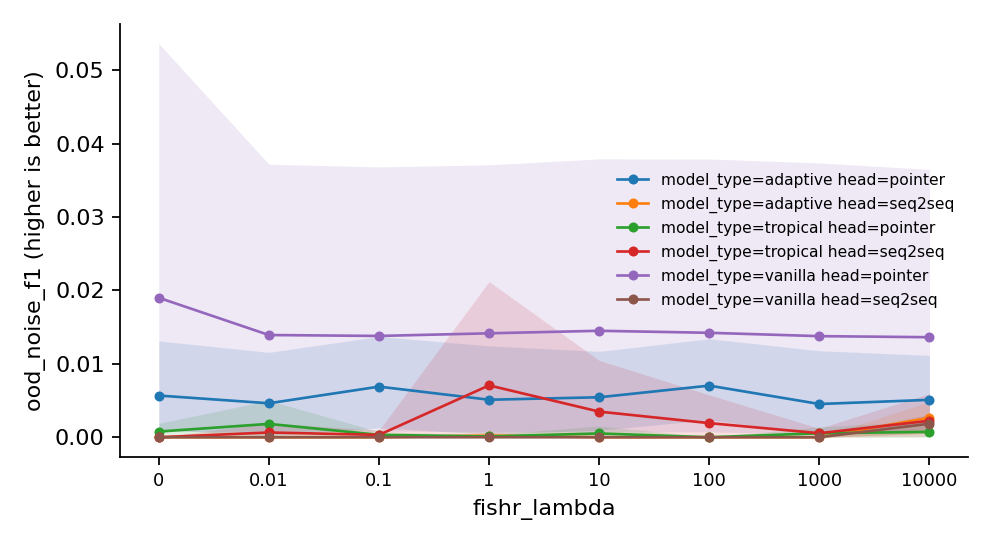
\includegraphics[width=\textwidth]{metric_ood_noise_f1.png}
\caption{\texttt{ood\_noise\_f1} against \texttt{fishr\_lambda}: the mean over seeds with a 95\% bootstrap CI, one line per combination of the other factors.}
\label{fig:ood_noise_f1}
\end{figure}

{\small
\begin{longtable}{lllrlrrr}
\caption{\texttt{ood\_noise\_f1} per cell: mean, 95\% bootstrap CI, SD, seeds, diverged runs.}\label{tab:summary-ood_noise_f1}\\
\toprule
\texttt{model\_type} & \texttt{head} & \texttt{fishr\_lambda} & mean & 95\% CI & SD & $n$ & div.\\
\midrule
\endhead
adaptive & pointer & 0 & 0.005681 & [0.00107, 0.0131] & 0.00836 & 5 & 0\\
adaptive & pointer & 0.01 & 0.004628 & [$2.15\times10^{-4}$, 0.0116] & 0.0076 & 5 & 0\\
adaptive & pointer & 0.1 & 0.006896 & [0.00128, 0.0137] & 0.00806 & 5 & 0\\
adaptive & pointer & 1 & 0.005111 & [$4.27\times10^{-4}$, 0.0124] & 0.00807 & 5 & 0\\
adaptive & pointer & 10 & 0.005446 & [$9.55\times10^{-4}$, 0.0117] & 0.00721 & 5 & 0\\
adaptive & pointer & 100 & 0.007034 & [0.00238, 0.0134] & 0.00746 & 5 & 0\\
adaptive & pointer & 1000 & 0.004529 & [$4.27\times10^{-4}$, 0.0118] & 0.00808 & 5 & 0\\
adaptive & pointer & 1e+04 & 0.005097 & [0.00107, 0.0112] & 0.00662 & 5 & 0\\
adaptive & seq2seq & 0 & 0 & [0, 0] & 0 & 5 & 0\\
adaptive & seq2seq & 0.01 & 0 & [0, 0] & 0 & 5 & 0\\
adaptive & seq2seq & 0.1 & 0 & [0, 0] & 0 & 5 & 0\\
adaptive & seq2seq & 1 & $2.247\times10^{-4}$ & [0, $6.74\times10^{-4}$] & $5.02\times10^{-4}$ & 5 & 0\\
adaptive & seq2seq & 10 & 0 & [0, 0] & 0 & 5 & 0\\
adaptive & seq2seq & 100 & 0 & [0, 0] & 0 & 5 & 0\\
adaptive & seq2seq & 1000 & 0 & [0, 0] & 0 & 5 & 0\\
adaptive & seq2seq & 1e+04 & 0.002666 & [$5.42\times10^{-4}$, 0.00484] & 0.00285 & 5 & 0\\
tropical & pointer & 0 & $7.762\times10^{-4}$ & [0, 0.0019] & 0.00122 & 5 & 0\\
tropical & pointer & 0.01 & 0.00182 & [0, 0.00501] & 0.00347 & 5 & 0\\
tropical & pointer & 0.1 & $3.261\times10^{-4}$ & [0, $7.54\times10^{-4}$] & $4.81\times10^{-4}$ & 5 & 0\\
tropical & pointer & 1 & $1.109\times10^{-4}$ & [0, $3.33\times10^{-4}$] & $2.48\times10^{-4}$ & 5 & 0\\
tropical & pointer & 10 & $5.168\times10^{-4}$ & [0, 0.00155] & 0.00116 & 5 & 0\\
tropical & pointer & 100 & 0 & [0, 0] & 0 & 5 & 0\\
tropical & pointer & 1000 & $5.438\times10^{-4}$ & [0, 0.00141] & $9.34\times10^{-4}$ & 5 & 0\\
tropical & pointer & 1e+04 & $7.388\times10^{-4}$ & [0, 0.00222] & 0.00165 & 5 & 0\\
tropical & seq2seq & 0 & 0 & [0, 0] & 0 & 5 & 0\\
tropical & seq2seq & 0.01 & $6.476\times10^{-4}$ & [0, 0.00194] & 0.00145 & 5 & 0\\
tropical & seq2seq & 0.1 & $3.223\times10^{-4}$ & [0, $9.67\times10^{-4}$] & $7.21\times10^{-4}$ & 5 & 0\\
tropical & seq2seq & 1 & 0.007066 & [0, 0.0212] & 0.0158 & 5 & 0\\
tropical & seq2seq & 10 & 0.003491 & [0, 0.0105] & 0.00781 & 5 & 0\\
tropical & seq2seq & 100 & 0.001924 & [0, 0.00577] & 0.0043 & 5 & 0\\
tropical & seq2seq & 1000 & $5.504\times10^{-4}$ & [0, 0.00122] & $7.83\times10^{-4}$ & 5 & 0\\
tropical & seq2seq & 1e+04 & 0.002246 & [$1.12\times10^{-4}$, 0.00595] & 0.00411 & 5 & 0\\
vanilla & pointer & 0 & 0.019 & [$7.56\times10^{-4}$, 0.0536] & 0.0387 & 5 & 0\\
vanilla & pointer & 0.01 & 0.01393 & [$8.48\times10^{-4}$, 0.0372] & 0.0257 & 5 & 0\\
vanilla & pointer & 0.1 & 0.0138 & [$8.46\times10^{-4}$, 0.0368] & 0.0255 & 5 & 0\\
vanilla & pointer & 1 & 0.01416 & [$7.36\times10^{-4}$, 0.0371] & 0.0253 & 5 & 0\\
vanilla & pointer & 10 & 0.0145 & [$7.37\times10^{-4}$, 0.0379] & 0.0258 & 5 & 0\\
vanilla & pointer & 100 & 0.01423 & [$7.34\times10^{-4}$, 0.0379] & 0.0262 & 5 & 0\\
vanilla & pointer & 1000 & 0.01377 & [$4.13\times10^{-4}$, 0.0374] & 0.026 & 5 & 0\\
vanilla & pointer & 1e+04 & 0.01363 & [$9.62\times10^{-4}$, 0.0365] & 0.0253 & 5 & 0\\
vanilla & seq2seq & 0 & 0 & [0, 0] & 0 & 5 & 0\\
vanilla & seq2seq & 0.01 & 0 & [0, 0] & 0 & 5 & 0\\
vanilla & seq2seq & 0.1 & 0 & [0, 0] & 0 & 5 & 0\\
vanilla & seq2seq & 1 & 0 & [0, 0] & 0 & 5 & 0\\
vanilla & seq2seq & 10 & 0 & [0, 0] & 0 & 5 & 0\\
vanilla & seq2seq & 100 & 0 & [0, 0] & 0 & 5 & 0\\
vanilla & seq2seq & 1000 & 0 & [0, 0] & 0 & 5 & 0\\
vanilla & seq2seq & 1e+04 & 0.001845 & [$5.42\times10^{-4}$, 0.00313] & 0.0017 & 5 & 0\\
\bottomrule
\end{longtable}
}

{\small
\begin{longtable}{lllrrrl}
\caption{\texttt{ood\_noise\_f1}: each level of \texttt{fishr\_lambda} against its control (0), within each combination of the other factors. rank: Wilcoxon signed-rank by seed, Holm.}\label{tab:control-ood_noise_f1}\\
\toprule
\texttt{model\_type} & \texttt{head} & \texttt{fishr\_lambda} & difference & 95\% CI & $p$ & \\
\midrule
\endhead
adaptive & pointer & 0.01 & -0.00256 & [-0.00262, 0.001] & 1.0000 & \\
adaptive & pointer & 0.1 & 0 & [-0.00132, 0.00406] & 1.0000 & \\
adaptive & pointer & 1 & -0.001292 & [-0.00215, 0.00138] & 1.0000 & \\
adaptive & pointer & 10 & $-3.779\times10^{-5}$ & [-0.00213, 0.00196] & 1.0000 & \\
adaptive & pointer & 100 & 0.002225 & [$-8.85\times10^{-4}$, 0.00359] & 1.0000 & \\
adaptive & pointer & 1000 & -0.001507 & [-0.0022, $-1.09\times10^{-4}$] & 1.0000 & \\
adaptive & pointer & 1e+04 & $-5.509\times10^{-4}$ & [-0.00278, 0.00157] & 1.0000 & \\
adaptive & seq2seq & 0.01 & 0 & [0, 0] & -- & \\
adaptive & seq2seq & 0.1 & 0 & [0, 0] & -- & \\
adaptive & seq2seq & 1 & 0 & [0, $6.74\times10^{-4}$] & 1.0000 & \\
adaptive & seq2seq & 10 & 0 & [0, 0] & -- & \\
adaptive & seq2seq & 100 & 0 & [0, 0] & -- & \\
adaptive & seq2seq & 1000 & 0 & [0, 0] & -- & \\
adaptive & seq2seq & 1e+04 & 0.002711 & [$5.42\times10^{-4}$, 0.00484] & 0.5000 & \\
tropical & pointer & 0.01 & 0 & [-0.00101, 0.00414] & 1.0000 & \\
tropical & pointer & 0.1 & 0 & [-0.00134, 0] & 1.0000 & \\
tropical & pointer & 1 & 0 & [-0.00177, $2.22\times10^{-4}$] & 1.0000 & \\
tropical & pointer & 10 & 0 & [-0.00168, $9.02\times10^{-4}$] & 1.0000 & \\
tropical & pointer & 100 & 0 & [-0.00177, 0] & 1.0000 & \\
tropical & pointer & 1000 & 0 & [-0.00157, $7.59\times10^{-4}$] & 1.0000 & \\
tropical & pointer & 1e+04 & 0 & [-0.00168, 0.00157] & 1.0000 & \\
tropical & seq2seq & 0.01 & 0 & [0, 0.00194] & 1.0000 & \\
tropical & seq2seq & 0.1 & 0 & [0, $9.67\times10^{-4}$] & 1.0000 & \\
tropical & seq2seq & 1 & 0 & [0, 0.0212] & 1.0000 & \\
tropical & seq2seq & 10 & 0 & [0, 0.0105] & 1.0000 & \\
tropical & seq2seq & 100 & 0 & [0, 0.00577] & 1.0000 & \\
tropical & seq2seq & 1000 & 0 & [0, 0.0012] & 1.0000 & \\
tropical & seq2seq & 1e+04 & $5.599\times10^{-4}$ & [$1.12\times10^{-4}$, 0.00595] & 1.0000 & \\
vanilla & pointer & 0.01 & 0 & [-0.017, 0.00224] & 1.0000 & \\
vanilla & pointer & 0.1 & 0 & [-0.0174, 0.00224] & 1.0000 & \\
vanilla & pointer & 1 & 0 & [-0.0175, 0.00343] & 1.0000 & \\
vanilla & pointer & 10 & 0 & [-0.0168, 0.00375] & 1.0000 & \\
vanilla & pointer & 100 & 0 & [-0.0164, 0.00256] & 1.0000 & \\
vanilla & pointer & 1000 & $-5.546\times10^{-4}$ & [-0.017, 0.00215] & 1.0000 & \\
vanilla & pointer & 1e+04 & 0 & [-0.0177, 0.00196] & 1.0000 & \\
vanilla & seq2seq & 0.01 & 0 & [0, 0] & -- & \\
vanilla & seq2seq & 0.1 & 0 & [0, 0] & -- & \\
vanilla & seq2seq & 1 & 0 & [0, 0] & -- & \\
vanilla & seq2seq & 10 & 0 & [0, 0] & -- & \\
vanilla & seq2seq & 100 & 0 & [0, 0] & -- & \\
vanilla & seq2seq & 1000 & 0 & [0, 0] & -- & \\
vanilla & seq2seq & 1e+04 & 0.002709 & [$5.42\times10^{-4}$, 0.0031] & 0.2500 & \\
\bottomrule
\end{longtable}
}

{\small
\begin{longtable}{llrrrrr}
\caption{\texttt{ood\_noise\_f1} against log10 \texttt{fishr\_lambda}: rank: Spearman rho, seed-bootstrap CI, with the Jonckheere--Terpstra ordered-trend $\tau$ and $p$.}\label{tab:trend-ood_noise_f1}\\
\toprule
\texttt{model\_type} & \texttt{head} & estimate & 95\% CI & $p$ & JT $\tau$ & JT $p$\\
\midrule
\endhead
adaptive & pointer & 0.04184 & [-0.198, 0.256] & 0.8114 & 0.0248 & 0.8658\\
adaptive & seq2seq & 0.3737 & [0.2, 0.549] & 0.0270 & 0.158 & 0.0262\\
tropical & pointer & -0.1197 & [-0.486, 0.171] & 0.4935 & -0.0762 & 0.4729\\
tropical & seq2seq & 0.204 & [-0.183, 0.667] & 0.2398 & 0.12 & 0.2631\\
vanilla & pointer & -0.009249 & [-0.0302, 0.0291] & 0.9579 & -0.00952 & 0.9462\\
vanilla & seq2seq & 0.4587 & [0.257, 0.611] & 0.0056 & 0.171 & 0.0034\\
\bottomrule
\end{longtable}
}

{\small
\begin{longtable}{lrrrl}
\caption{\texttt{ood\_noise\_f1}: paired contrasts by seed, Holm-corrected across the cells. rank: Wilcoxon signed-rank by seed, Holm.}\label{tab:paired-ood_noise_f1}\\
\toprule
contrast (within) & difference & 95\% CI & $p$ & \\
\midrule
\endhead
\stackcell{model\_type: tropical - vanilla\\\footnotesize head=pointer fishr\_lambda=0 } & -0.01823 & [-0.0668, 0.0304] & 1.0000 & \\
\stackcell{model\_type: tropical - vanilla\\\footnotesize head=pointer fishr\_lambda=0.01 } & -0.01211 & [-0.0452, 0.021] & 1.0000 & \\
\stackcell{model\_type: tropical - vanilla\\\footnotesize head=pointer fishr\_lambda=0.1 } & -0.01347 & [-0.0453, 0.0183] & 1.0000 & \\
\stackcell{model\_type: tropical - vanilla\\\footnotesize head=pointer fishr\_lambda=1 } & -0.01405 & [-0.0451, 0.017] & 1.0000 & \\
\stackcell{model\_type: tropical - vanilla\\\footnotesize head=pointer fishr\_lambda=10 } & -0.01399 & [-0.0462, 0.0182] & 1.0000 & \\
\stackcell{model\_type: tropical - vanilla\\\footnotesize head=pointer fishr\_lambda=100 } & -0.01423 & [-0.0467, 0.0182] & 1.0000 & \\
\stackcell{model\_type: tropical - vanilla\\\footnotesize head=pointer fishr\_lambda=1000 } & -0.01323 & [-0.0458, 0.0193] & 1.0000 & \\
\stackcell{model\_type: tropical - vanilla\\\footnotesize head=pointer fishr\_lambda=1e+04 } & -0.01289 & [-0.0447, 0.0189] & 1.0000 & \\
\stackcell{model\_type: tropical - vanilla\\\footnotesize head=seq2seq fishr\_lambda=0 } & 0 & [--, --] & -- & \\
\stackcell{model\_type: tropical - vanilla\\\footnotesize head=seq2seq fishr\_lambda=0.01 } & $6.476\times10^{-4}$ & [-0.00115, 0.00245] & 1.0000 & \\
\stackcell{model\_type: tropical - vanilla\\\footnotesize head=seq2seq fishr\_lambda=0.1 } & $3.223\times10^{-4}$ & [$-5.73\times10^{-4}$, 0.00122] & 1.0000 & \\
\stackcell{model\_type: tropical - vanilla\\\footnotesize head=seq2seq fishr\_lambda=1 } & 0.007066 & [-0.0126, 0.0267] & 1.0000 & \\
\stackcell{model\_type: tropical - vanilla\\\footnotesize head=seq2seq fishr\_lambda=10 } & 0.003491 & [-0.0062, 0.0132] & 1.0000 & \\
\stackcell{model\_type: tropical - vanilla\\\footnotesize head=seq2seq fishr\_lambda=100 } & 0.001924 & [-0.00342, 0.00726] & 1.0000 & \\
\stackcell{model\_type: tropical - vanilla\\\footnotesize head=seq2seq fishr\_lambda=1000 } & $5.504\times10^{-4}$ & [$-4.21\times10^{-4}$, 0.00152] & 1.0000 & \\
\stackcell{model\_type: tropical - vanilla\\\footnotesize head=seq2seq fishr\_lambda=1e+04 } & $4.002\times10^{-4}$ & [-0.00631, 0.00711] & 1.0000 & \\
\stackcell{model\_type: adaptive - vanilla\\\footnotesize head=pointer fishr\_lambda=0 } & -0.01332 & [-0.0512, 0.0245] & 1.0000 & \\
\stackcell{model\_type: adaptive - vanilla\\\footnotesize head=pointer fishr\_lambda=0.01 } & -0.009297 & [-0.0323, 0.0137] & 1.0000 & \\
\stackcell{model\_type: adaptive - vanilla\\\footnotesize head=pointer fishr\_lambda=0.1 } & -0.006905 & [-0.0295, 0.0157] & 1.0000 & \\
\stackcell{model\_type: adaptive - vanilla\\\footnotesize head=pointer fishr\_lambda=1 } & -0.009049 & [-0.031, 0.0129] & 1.0000 & \\
\stackcell{model\_type: adaptive - vanilla\\\footnotesize head=pointer fishr\_lambda=10 } & -0.009057 & [-0.0326, 0.0145] & 1.0000 & \\
\stackcell{model\_type: adaptive - vanilla\\\footnotesize head=pointer fishr\_lambda=100 } & -0.007195 & [-0.0307, 0.0163] & 1.0000 & \\
\stackcell{model\_type: adaptive - vanilla\\\footnotesize head=pointer fishr\_lambda=1000 } & -0.009245 & [-0.0316, 0.0132] & 1.0000 & \\
\stackcell{model\_type: adaptive - vanilla\\\footnotesize head=pointer fishr\_lambda=1e+04 } & -0.008532 & [-0.0321, 0.0151] & 1.0000 & \\
\stackcell{model\_type: adaptive - vanilla\\\footnotesize head=seq2seq fishr\_lambda=0 } & 0 & [--, --] & -- & \\
\stackcell{model\_type: adaptive - vanilla\\\footnotesize head=seq2seq fishr\_lambda=0.01 } & 0 & [--, --] & -- & \\
\stackcell{model\_type: adaptive - vanilla\\\footnotesize head=seq2seq fishr\_lambda=0.1 } & 0 & [--, --] & -- & \\
\stackcell{model\_type: adaptive - vanilla\\\footnotesize head=seq2seq fishr\_lambda=1 } & $2.247\times10^{-4}$ & [$-3.99\times10^{-4}$, $8.49\times10^{-4}$] & 1.0000 & \\
\stackcell{model\_type: adaptive - vanilla\\\footnotesize head=seq2seq fishr\_lambda=10 } & 0 & [--, --] & -- & \\
\stackcell{model\_type: adaptive - vanilla\\\footnotesize head=seq2seq fishr\_lambda=100 } & 0 & [--, --] & -- & \\
\stackcell{model\_type: adaptive - vanilla\\\footnotesize head=seq2seq fishr\_lambda=1000 } & 0 & [--, --] & -- & \\
\stackcell{model\_type: adaptive - vanilla\\\footnotesize head=seq2seq fishr\_lambda=1e+04 } & $8.210\times10^{-4}$ & [-0.00111, 0.00276] & 1.0000 & \\
\stackcell{head: pointer - seq2seq\\\footnotesize model\_type=adaptive fishr\_lambda=0 } & 0.005681 & [-0.00469, 0.0161] & 1.0000 & \\
\stackcell{head: pointer - seq2seq\\\footnotesize model\_type=adaptive fishr\_lambda=0.01 } & 0.004628 & [-0.00481, 0.0141] & 1.0000 & \\
\stackcell{head: pointer - seq2seq\\\footnotesize model\_type=adaptive fishr\_lambda=0.1 } & 0.006896 & [-0.00311, 0.0169] & 1.0000 & \\
\stackcell{head: pointer - seq2seq\\\footnotesize model\_type=adaptive fishr\_lambda=1 } & 0.004886 & [-0.00537, 0.0151] & 1.0000 & \\
\stackcell{head: pointer - seq2seq\\\footnotesize model\_type=adaptive fishr\_lambda=10 } & 0.005446 & [-0.00351, 0.0144] & 1.0000 & \\
\stackcell{head: pointer - seq2seq\\\footnotesize model\_type=adaptive fishr\_lambda=100 } & 0.007034 & [-0.00223, 0.0163] & 1.0000 & \\
\stackcell{head: pointer - seq2seq\\\footnotesize model\_type=adaptive fishr\_lambda=1000 } & 0.004529 & [-0.00551, 0.0146] & 1.0000 & \\
\stackcell{head: pointer - seq2seq\\\footnotesize model\_type=adaptive fishr\_lambda=1e+04 } & 0.00243 & [-0.0071, 0.012] & 1.0000 & \\
\stackcell{head: pointer - seq2seq\\\footnotesize model\_type=tropical fishr\_lambda=0 } & $7.762\times10^{-4}$ & [$-7.44\times10^{-4}$, 0.0023] & 1.0000 & \\
\stackcell{head: pointer - seq2seq\\\footnotesize model\_type=tropical fishr\_lambda=0.01 } & 0.001172 & [-0.00397, 0.00631] & 1.0000 & \\
\stackcell{head: pointer - seq2seq\\\footnotesize model\_type=tropical fishr\_lambda=0.1 } & $3.740\times10^{-6}$ & [-0.00125, 0.00125] & 1.0000 & \\
\stackcell{head: pointer - seq2seq\\\footnotesize model\_type=tropical fishr\_lambda=1 } & -0.006956 & [-0.0267, 0.0127] & 1.0000 & \\
\stackcell{head: pointer - seq2seq\\\footnotesize model\_type=tropical fishr\_lambda=10 } & -0.002974 & [-0.0131, 0.00717] & 1.0000 & \\
\stackcell{head: pointer - seq2seq\\\footnotesize model\_type=tropical fishr\_lambda=100 } & -0.001924 & [-0.00726, 0.00342] & 1.0000 & \\
\stackcell{head: pointer - seq2seq\\\footnotesize model\_type=tropical fishr\_lambda=1000 } & $-6.569\times10^{-6}$ & [-0.00186, 0.00185] & 1.0000 & \\
\stackcell{head: pointer - seq2seq\\\footnotesize model\_type=tropical fishr\_lambda=1e+04 } & -0.001507 & [-0.00458, 0.00156] & 1.0000 & \\
\stackcell{head: pointer - seq2seq\\\footnotesize model\_type=vanilla fishr\_lambda=0 } & 0.019 & [-0.029, 0.067] & 1.0000 & \\
\stackcell{head: pointer - seq2seq\\\footnotesize model\_type=vanilla fishr\_lambda=0.01 } & 0.01393 & [-0.018, 0.0459] & 1.0000 & \\
\stackcell{head: pointer - seq2seq\\\footnotesize model\_type=vanilla fishr\_lambda=0.1 } & 0.0138 & [-0.0178, 0.0454] & 1.0000 & \\
\stackcell{head: pointer - seq2seq\\\footnotesize model\_type=vanilla fishr\_lambda=1 } & 0.01416 & [-0.0172, 0.0455] & 1.0000 & \\
\stackcell{head: pointer - seq2seq\\\footnotesize model\_type=vanilla fishr\_lambda=10 } & 0.0145 & [-0.0175, 0.0465] & 1.0000 & \\
\stackcell{head: pointer - seq2seq\\\footnotesize model\_type=vanilla fishr\_lambda=100 } & 0.01423 & [-0.0182, 0.0467] & 1.0000 & \\
\stackcell{head: pointer - seq2seq\\\footnotesize model\_type=vanilla fishr\_lambda=1000 } & 0.01377 & [-0.0185, 0.0461] & 1.0000 & \\
\stackcell{head: pointer - seq2seq\\\footnotesize model\_type=vanilla fishr\_lambda=1e+04 } & 0.01178 & [-0.0193, 0.0429] & 1.0000 & \\
\bottomrule
\end{longtable}
}

\subsection{\texttt{ood\_noise\_exact}}
\begin{figure}[tbp]
\centering
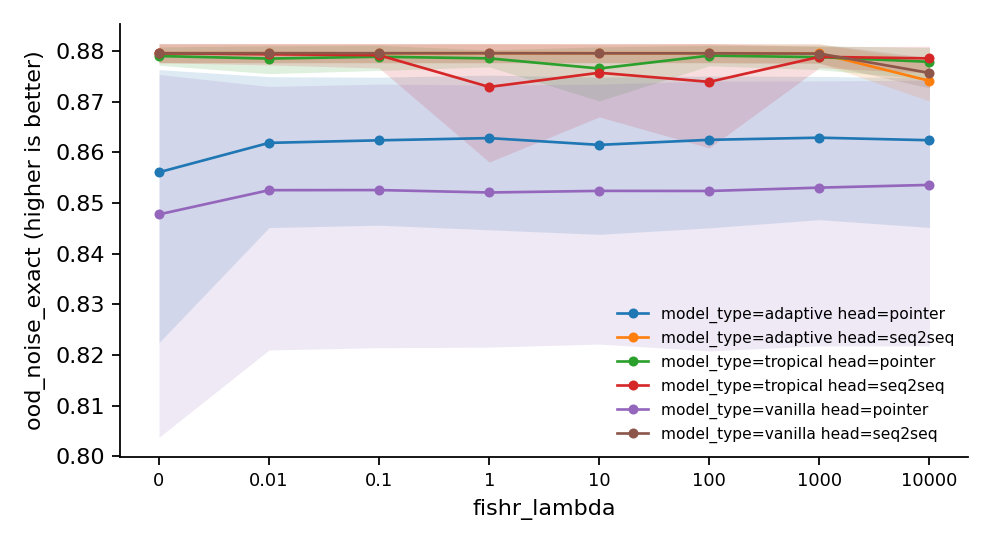
\includegraphics[width=\textwidth]{metric_ood_noise_exact.png}
\caption{\texttt{ood\_noise\_exact} against \texttt{fishr\_lambda}: the mean over seeds with a 95\% bootstrap CI, one line per combination of the other factors.}
\label{fig:ood_noise_exact}
\end{figure}

{\small
\begin{longtable}{lllrlrrr}
\caption{\texttt{ood\_noise\_exact} per cell: mean, 95\% bootstrap CI, SD, seeds, diverged runs.}\label{tab:summary-ood_noise_exact}\\
\toprule
\texttt{model\_type} & \texttt{head} & \texttt{fishr\_lambda} & mean & 95\% CI & SD & $n$ & div.\\
\midrule
\endhead
adaptive & pointer & 0 & 0.8561 & [0.822, 0.876] & 0.0375 & 5 & 0\\
adaptive & pointer & 0.01 & 0.8619 & [0.845, 0.875] & 0.0195 & 5 & 0\\
adaptive & pointer & 0.1 & 0.8624 & [0.846, 0.875] & 0.0196 & 5 & 0\\
adaptive & pointer & 1 & 0.8628 & [0.845, 0.875] & 0.0209 & 5 & 0\\
adaptive & pointer & 10 & 0.8615 & [0.844, 0.875] & 0.0205 & 5 & 0\\
adaptive & pointer & 100 & 0.8625 & [0.845, 0.875] & 0.02 & 5 & 0\\
adaptive & pointer & 1000 & 0.8629 & [0.847, 0.875] & 0.0187 & 5 & 0\\
adaptive & pointer & 1e+04 & 0.8624 & [0.845, 0.875] & 0.0188 & 5 & 0\\
adaptive & seq2seq & 0 & 0.8796 & [0.878, 0.881] & 0.0025 & 5 & 0\\
adaptive & seq2seq & 0.01 & 0.8796 & [0.878, 0.881] & 0.0025 & 5 & 0\\
adaptive & seq2seq & 0.1 & 0.8796 & [0.878, 0.881] & 0.00248 & 5 & 0\\
adaptive & seq2seq & 1 & 0.8796 & [0.878, 0.881] & 0.0025 & 5 & 0\\
adaptive & seq2seq & 10 & 0.8796 & [0.878, 0.881] & 0.0025 & 5 & 0\\
adaptive & seq2seq & 100 & 0.8796 & [0.878, 0.881] & 0.0025 & 5 & 0\\
adaptive & seq2seq & 1000 & 0.8795 & [0.878, 0.881] & 0.00256 & 5 & 0\\
adaptive & seq2seq & 1e+04 & 0.8741 & [0.87, 0.878] & 0.00549 & 5 & 0\\
tropical & pointer & 0 & 0.879 & [0.877, 0.881] & 0.00235 & 5 & 0\\
tropical & pointer & 0.01 & 0.8785 & [0.876, 0.881] & 0.00342 & 5 & 0\\
tropical & pointer & 0.1 & 0.8789 & [0.876, 0.881] & 0.00317 & 5 & 0\\
tropical & pointer & 1 & 0.8786 & [0.877, 0.88] & 0.00219 & 5 & 0\\
tropical & pointer & 10 & 0.8766 & [0.87, 0.881] & 0.00713 & 5 & 0\\
tropical & pointer & 100 & 0.8791 & [0.877, 0.881] & 0.0026 & 5 & 0\\
tropical & pointer & 1000 & 0.8788 & [0.876, 0.881] & 0.00306 & 5 & 0\\
tropical & pointer & 1e+04 & 0.8779 & [0.874, 0.881] & 0.00435 & 5 & 0\\
tropical & seq2seq & 0 & 0.8796 & [0.878, 0.881] & 0.0025 & 5 & 0\\
tropical & seq2seq & 0.01 & 0.8794 & [0.877, 0.881] & 0.0028 & 5 & 0\\
tropical & seq2seq & 0.1 & 0.8792 & [0.877, 0.881] & 0.00309 & 5 & 0\\
tropical & seq2seq & 1 & 0.8729 & [0.858, 0.881] & 0.0162 & 5 & 0\\
tropical & seq2seq & 10 & 0.8757 & [0.867, 0.881] & 0.0103 & 5 & 0\\
tropical & seq2seq & 100 & 0.8739 & [0.861, 0.881] & 0.0143 & 5 & 0\\
tropical & seq2seq & 1000 & 0.8789 & [0.877, 0.881] & 0.00274 & 5 & 0\\
tropical & seq2seq & 1e+04 & 0.8786 & [0.876, 0.881] & 0.00337 & 5 & 0\\
vanilla & pointer & 0 & 0.8478 & [0.804, 0.875] & 0.0512 & 5 & 0\\
vanilla & pointer & 0.01 & 0.8525 & [0.821, 0.873] & 0.0354 & 5 & 0\\
vanilla & pointer & 0.1 & 0.8526 & [0.821, 0.873] & 0.0349 & 5 & 0\\
vanilla & pointer & 1 & 0.8521 & [0.822, 0.873] & 0.0342 & 5 & 0\\
vanilla & pointer & 10 & 0.8524 & [0.822, 0.873] & 0.0344 & 5 & 0\\
vanilla & pointer & 100 & 0.8524 & [0.821, 0.874] & 0.0354 & 5 & 0\\
vanilla & pointer & 1000 & 0.853 & [0.822, 0.874] & 0.035 & 5 & 0\\
vanilla & pointer & 1e+04 & 0.8536 & [0.822, 0.874] & 0.0355 & 5 & 0\\
vanilla & seq2seq & 0 & 0.8796 & [0.878, 0.881] & 0.0025 & 5 & 0\\
vanilla & seq2seq & 0.01 & 0.8796 & [0.878, 0.881] & 0.0025 & 5 & 0\\
vanilla & seq2seq & 0.1 & 0.8796 & [0.878, 0.881] & 0.0025 & 5 & 0\\
vanilla & seq2seq & 1 & 0.8796 & [0.878, 0.881] & 0.0025 & 5 & 0\\
vanilla & seq2seq & 10 & 0.8796 & [0.878, 0.881] & 0.00248 & 5 & 0\\
vanilla & seq2seq & 100 & 0.8796 & [0.878, 0.881] & 0.00248 & 5 & 0\\
vanilla & seq2seq & 1000 & 0.8795 & [0.878, 0.881] & 0.00256 & 5 & 0\\
vanilla & seq2seq & 1e+04 & 0.8757 & [0.873, 0.879] & 0.00396 & 5 & 0\\
\bottomrule
\end{longtable}
}

{\small
\begin{longtable}{lllrrrl}
\caption{\texttt{ood\_noise\_exact}: each level of \texttt{fishr\_lambda} against its control (0), within each combination of the other factors. parametric: Dunnett vs control.}\label{tab:control-ood_noise_exact}\\
\toprule
\texttt{model\_type} & \texttt{head} & \texttt{fishr\_lambda} & difference & 95\% CI & $p$ & \\
\midrule
\endhead
adaptive & pointer & 0.01 & 0.0058 & [-0.0339, 0.0455] & 0.9987 & \\
adaptive & pointer & 0.1 & 0.0063 & [-0.0334, 0.046] & 0.9979 & \\
adaptive & pointer & 1 & 0.00674 & [-0.033, 0.0464] & 0.9968 & \\
adaptive & pointer & 10 & 0.0054 & [-0.0343, 0.0451] & 0.9992 & \\
adaptive & pointer & 100 & 0.0064 & [-0.0333, 0.0461] & 0.9977 & \\
adaptive & pointer & 1000 & 0.00682 & [-0.0329, 0.0465] & 0.9966 & \\
adaptive & pointer & 1e+04 & 0.00632 & [-0.0334, 0.046] & 0.9979 & \\
adaptive & seq2seq & 0.01 & 0 & [-0.00532, 0.00532] & 1.0000 & \\
adaptive & seq2seq & 0.1 & $-2.000\times10^{-5}$ & [-0.00534, 0.0053] & 1.0000 & \\
adaptive & seq2seq & 1 & 0 & [-0.00532, 0.00532] & 1.0000 & \\
adaptive & seq2seq & 10 & 0 & [-0.00532, 0.00532] & 1.0000 & \\
adaptive & seq2seq & 100 & 0 & [-0.00532, 0.00532] & 1.0000 & \\
adaptive & seq2seq & 1000 & $-4.000\times10^{-5}$ & [-0.00536, 0.00528] & 1.0000 & \\
adaptive & seq2seq & 1e+04 & -0.00546 & [-0.0108, $-1.43\times10^{-4}$] & 0.0423 & *\\
tropical & pointer & 0.01 & $-5.000\times10^{-4}$ & [-0.00721, 0.00621] & 1.0000 & \\
tropical & pointer & 0.1 & $-1.400\times10^{-4}$ & [-0.00685, 0.00657] & 1.0000 & \\
tropical & pointer & 1 & $-4.600\times10^{-4}$ & [-0.00717, 0.00625] & 1.0000 & \\
tropical & pointer & 10 & -0.00246 & [-0.00917, 0.00425] & 0.8473 & \\
tropical & pointer & 100 & $8.000\times10^{-5}$ & [-0.00663, 0.00679] & 1.0000 & \\
tropical & pointer & 1000 & $-2.200\times10^{-4}$ & [-0.00693, 0.00649] & 1.0000 & \\
tropical & pointer & 1e+04 & -0.00114 & [-0.00785, 0.00557] & 0.9968 & \\
tropical & seq2seq & 0.01 & $-2.200\times10^{-4}$ & [-0.0155, 0.0151] & 1.0000 & \\
tropical & seq2seq & 0.1 & $-4.000\times10^{-4}$ & [-0.0157, 0.0149] & 1.0000 & \\
tropical & seq2seq & 1 & -0.00666 & [-0.022, 0.00865] & 0.7279 & \\
tropical & seq2seq & 10 & -0.00386 & [-0.0192, 0.0115] & 0.9711 & \\
tropical & seq2seq & 100 & -0.00566 & [-0.021, 0.00965] & 0.8427 & \\
tropical & seq2seq & 1000 & $-7.200\times10^{-4}$ & [-0.016, 0.0146] & 1.0000 & \\
tropical & seq2seq & 1e+04 & -0.00102 & [-0.0163, 0.0143] & 1.0000 & \\
vanilla & pointer & 0.01 & 0.00478 & [-0.0605, 0.0701] & 1.0000 & \\
vanilla & pointer & 0.1 & 0.0048 & [-0.0605, 0.0701] & 1.0000 & \\
vanilla & pointer & 1 & 0.00432 & [-0.061, 0.0696] & 1.0000 & \\
vanilla & pointer & 10 & 0.00464 & [-0.0607, 0.0699] & 1.0000 & \\
vanilla & pointer & 100 & 0.00462 & [-0.0607, 0.0699] & 1.0000 & \\
vanilla & pointer & 1000 & 0.00528 & [-0.06, 0.0706] & 1.0000 & \\
vanilla & pointer & 1e+04 & 0.00582 & [-0.0595, 0.0711] & 0.9999 & \\
vanilla & seq2seq & 0.01 & 0 & [-0.00477, 0.00477] & 1.0000 & \\
vanilla & seq2seq & 0.1 & 0 & [-0.00477, 0.00477] & 1.0000 & \\
vanilla & seq2seq & 1 & 0 & [-0.00477, 0.00477] & 1.0000 & \\
vanilla & seq2seq & 10 & $-2.000\times10^{-5}$ & [-0.00479, 0.00475] & 1.0000 & \\
vanilla & seq2seq & 100 & $-2.000\times10^{-5}$ & [-0.00479, 0.00475] & 1.0000 & \\
vanilla & seq2seq & 1000 & $-8.000\times10^{-5}$ & [-0.00485, 0.00469] & 1.0000 & \\
vanilla & seq2seq & 1e+04 & -0.0039 & [-0.00867, $8.67\times10^{-4}$] & 0.1458 & \\
\bottomrule
\end{longtable}
}

{\small
\begin{longtable}{llrrrrr}
\caption{\texttt{ood\_noise\_exact} against log10 \texttt{fishr\_lambda}: parametric: OLS slope t-test, seed-bootstrap CI, with the Jonckheere--Terpstra ordered-trend $\tau$ and $p$.}\label{tab:trend-ood_noise_exact}\\
\toprule
\texttt{model\_type} & \texttt{head} & estimate & 95\% CI & $p$ & JT $\tau$ & JT $p$\\
\midrule
\endhead
adaptive & pointer & $8.071\times10^{-5}$ & [$-5.14\times10^{-5}$, $2.57\times10^{-4}$] & 0.9584 & -0.00762 & 0.9666\\
adaptive & seq2seq & $-5.864\times10^{-4}$ & [$-9.98\times10^{-4}$, $-1.75\times10^{-4}$] & 0.0408 & -0.261 & 0.0492\\
tropical & pointer & $-5.500\times10^{-5}$ & [$-1.24\times10^{-4}$, $1.43\times10^{-5}$] & 0.8645 & -0.0381 & 0.7734\\
tropical & seq2seq & $-7.286\times10^{-5}$ & [$-2.21\times10^{-4}$, $8.14\times10^{-5}$] & 0.9240 & -0.0838 & 0.5229\\
vanilla & pointer & $1.564\times10^{-4}$ & [$4.29\times10^{-6}$, $3.37\times10^{-4}$] & 0.9545 & 0.0495 & 0.7209\\
vanilla & seq2seq & $-4.243\times10^{-4}$ & [$-7.35\times10^{-4}$, $-1.48\times10^{-4}$] & 0.0787 & -0.227 & 0.0892\\
\bottomrule
\end{longtable}
}

{\small
\begin{longtable}{lrrrl}
\caption{\texttt{ood\_noise\_exact}: paired contrasts by seed, Holm-corrected across the cells. parametric: paired t-test by seed, Holm.}\label{tab:paired-ood_noise_exact}\\
\toprule
contrast (within) & difference & 95\% CI & $p$ & \\
\midrule
\endhead
\stackcell{model\_type: tropical - vanilla\\\footnotesize head=pointer fishr\_lambda=0 } & 0.03126 & [-0.0331, 0.0957] & 1.0000 & \\
\stackcell{model\_type: tropical - vanilla\\\footnotesize head=pointer fishr\_lambda=0.01 } & 0.02598 & [-0.0194, 0.0714] & 1.0000 & \\
\stackcell{model\_type: tropical - vanilla\\\footnotesize head=pointer fishr\_lambda=0.1 } & 0.02632 & [-0.0187, 0.0714] & 1.0000 & \\
\stackcell{model\_type: tropical - vanilla\\\footnotesize head=pointer fishr\_lambda=1 } & 0.02648 & [-0.0155, 0.0684] & 1.0000 & \\
\stackcell{model\_type: tropical - vanilla\\\footnotesize head=pointer fishr\_lambda=10 } & 0.02416 & [-0.0216, 0.0699] & 1.0000 & \\
\stackcell{model\_type: tropical - vanilla\\\footnotesize head=pointer fishr\_lambda=100 } & 0.02672 & [-0.0185, 0.0719] & 1.0000 & \\
\stackcell{model\_type: tropical - vanilla\\\footnotesize head=pointer fishr\_lambda=1000 } & 0.02576 & [-0.0194, 0.0709] & 1.0000 & \\
\stackcell{model\_type: tropical - vanilla\\\footnotesize head=pointer fishr\_lambda=1e+04 } & 0.0243 & [-0.0215, 0.0701] & 1.0000 & \\
\stackcell{model\_type: tropical - vanilla\\\footnotesize head=seq2seq fishr\_lambda=0 } & 0 & [--, --] & -- & \\
\stackcell{model\_type: tropical - vanilla\\\footnotesize head=seq2seq fishr\_lambda=0.01 } & $-2.200\times10^{-4}$ & [$-5.97\times10^{-4}$, $1.57\times10^{-4}$] & 1.0000 & \\
\stackcell{model\_type: tropical - vanilla\\\footnotesize head=seq2seq fishr\_lambda=0.1 } & $-4.000\times10^{-4}$ & [-0.00138, $5.78\times10^{-4}$] & 1.0000 & \\
\stackcell{model\_type: tropical - vanilla\\\footnotesize head=seq2seq fishr\_lambda=1 } & -0.00666 & [-0.0247, 0.0113] & 1.0000 & \\
\stackcell{model\_type: tropical - vanilla\\\footnotesize head=seq2seq fishr\_lambda=10 } & -0.00384 & [-0.0146, 0.00689] & 1.0000 & \\
\stackcell{model\_type: tropical - vanilla\\\footnotesize head=seq2seq fishr\_lambda=100 } & -0.00564 & [-0.0214, 0.0101] & 1.0000 & \\
\stackcell{model\_type: tropical - vanilla\\\footnotesize head=seq2seq fishr\_lambda=1000 } & $-6.400\times10^{-4}$ & [-0.00183, $5.46\times10^{-4}$] & 1.0000 & \\
\stackcell{model\_type: tropical - vanilla\\\footnotesize head=seq2seq fishr\_lambda=1e+04 } & 0.00288 & [-0.00288, 0.00864] & 1.0000 & \\
\stackcell{model\_type: adaptive - vanilla\\\footnotesize head=pointer fishr\_lambda=0 } & 0.00832 & [-0.0109, 0.0275] & 1.0000 & \\
\stackcell{model\_type: adaptive - vanilla\\\footnotesize head=pointer fishr\_lambda=0.01 } & 0.00934 & [-0.0111, 0.0297] & 1.0000 & \\
\stackcell{model\_type: adaptive - vanilla\\\footnotesize head=pointer fishr\_lambda=0.1 } & 0.00982 & [-0.00943, 0.0291] & 1.0000 & \\
\stackcell{model\_type: adaptive - vanilla\\\footnotesize head=pointer fishr\_lambda=1 } & 0.01074 & [-0.00601, 0.0275] & 1.0000 & \\
\stackcell{model\_type: adaptive - vanilla\\\footnotesize head=pointer fishr\_lambda=10 } & 0.00908 & [-0.00857, 0.0267] & 1.0000 & \\
\stackcell{model\_type: adaptive - vanilla\\\footnotesize head=pointer fishr\_lambda=100 } & 0.0101 & [-0.00929, 0.0295] & 1.0000 & \\
\stackcell{model\_type: adaptive - vanilla\\\footnotesize head=pointer fishr\_lambda=1000 } & 0.00986 & [-0.0108, 0.0305] & 1.0000 & \\
\stackcell{model\_type: adaptive - vanilla\\\footnotesize head=pointer fishr\_lambda=1e+04 } & 0.00882 & [-0.0124, 0.03] & 1.0000 & \\
\stackcell{model\_type: adaptive - vanilla\\\footnotesize head=seq2seq fishr\_lambda=0 } & 0 & [--, --] & -- & \\
\stackcell{model\_type: adaptive - vanilla\\\footnotesize head=seq2seq fishr\_lambda=0.01 } & 0 & [--, --] & -- & \\
\stackcell{model\_type: adaptive - vanilla\\\footnotesize head=seq2seq fishr\_lambda=0.1 } & $-2.000\times10^{-5}$ & [$-7.55\times10^{-5}$, $3.55\times10^{-5}$] & 1.0000 & \\
\stackcell{model\_type: adaptive - vanilla\\\footnotesize head=seq2seq fishr\_lambda=1 } & 0 & [--, --] & -- & \\
\stackcell{model\_type: adaptive - vanilla\\\footnotesize head=seq2seq fishr\_lambda=10 } & $2.000\times10^{-5}$ & [$-3.55\times10^{-5}$, $7.55\times10^{-5}$] & 1.0000 & \\
\stackcell{model\_type: adaptive - vanilla\\\footnotesize head=seq2seq fishr\_lambda=100 } & $2.000\times10^{-5}$ & [$-3.55\times10^{-5}$, $7.55\times10^{-5}$] & 1.0000 & \\
\stackcell{model\_type: adaptive - vanilla\\\footnotesize head=seq2seq fishr\_lambda=1000 } & $4.000\times10^{-5}$ & [$-2.80\times10^{-5}$, $1.08\times10^{-4}$] & 1.0000 & \\
\stackcell{model\_type: adaptive - vanilla\\\footnotesize head=seq2seq fishr\_lambda=1e+04 } & -0.00156 & [-0.005, 0.00188] & 1.0000 & \\
\stackcell{head: pointer - seq2seq\\\footnotesize model\_type=adaptive fishr\_lambda=0 } & -0.0235 & [-0.071, 0.024] & 1.0000 & \\
\stackcell{head: pointer - seq2seq\\\footnotesize model\_type=adaptive fishr\_lambda=0.01 } & -0.0177 & [-0.0434, 0.00801] & 1.0000 & \\
\stackcell{head: pointer - seq2seq\\\footnotesize model\_type=adaptive fishr\_lambda=0.1 } & -0.01718 & [-0.0429, 0.0085] & 1.0000 & \\
\stackcell{head: pointer - seq2seq\\\footnotesize model\_type=adaptive fishr\_lambda=1 } & -0.01676 & [-0.0439, 0.0104] & 1.0000 & \\
\stackcell{head: pointer - seq2seq\\\footnotesize model\_type=adaptive fishr\_lambda=10 } & -0.0181 & [-0.0448, 0.00864] & 1.0000 & \\
\stackcell{head: pointer - seq2seq\\\footnotesize model\_type=adaptive fishr\_lambda=100 } & -0.0171 & [-0.0433, 0.00908] & 1.0000 & \\
\stackcell{head: pointer - seq2seq\\\footnotesize model\_type=adaptive fishr\_lambda=1000 } & -0.01664 & [-0.0413, 0.00803] & 1.0000 & \\
\stackcell{head: pointer - seq2seq\\\footnotesize model\_type=adaptive fishr\_lambda=1e+04 } & -0.01172 & [-0.036, 0.0126] & 1.0000 & \\
\stackcell{head: pointer - seq2seq\\\footnotesize model\_type=tropical fishr\_lambda=0 } & $-5.600\times10^{-4}$ & [-0.00117, $5.21\times10^{-5}$] & 1.0000 & \\
\stackcell{head: pointer - seq2seq\\\footnotesize model\_type=tropical fishr\_lambda=0.01 } & $-8.400\times10^{-4}$ & [-0.0024, $7.25\times10^{-4}$] & 1.0000 & \\
\stackcell{head: pointer - seq2seq\\\footnotesize model\_type=tropical fishr\_lambda=0.1 } & $-3.000\times10^{-4}$ & [-0.00206, 0.00146] & 1.0000 & \\
\stackcell{head: pointer - seq2seq\\\footnotesize model\_type=tropical fishr\_lambda=1 } & 0.00564 & [-0.013, 0.0243] & 1.0000 & \\
\stackcell{head: pointer - seq2seq\\\footnotesize model\_type=tropical fishr\_lambda=10 } & $8.400\times10^{-4}$ & [-0.0131, 0.0148] & 1.0000 & \\
\stackcell{head: pointer - seq2seq\\\footnotesize model\_type=tropical fishr\_lambda=100 } & 0.00518 & [-0.0105, 0.0208] & 1.0000 & \\
\stackcell{head: pointer - seq2seq\\\footnotesize model\_type=tropical fishr\_lambda=1000 } & $-6.000\times10^{-5}$ & [-0.00143, 0.00131] & 1.0000 & \\
\stackcell{head: pointer - seq2seq\\\footnotesize model\_type=tropical fishr\_lambda=1e+04 } & $-6.800\times10^{-4}$ & [-0.00237, 0.00101] & 1.0000 & \\
\stackcell{head: pointer - seq2seq\\\footnotesize model\_type=vanilla fishr\_lambda=0 } & -0.03182 & [-0.0967, 0.0331] & 1.0000 & \\
\stackcell{head: pointer - seq2seq\\\footnotesize model\_type=vanilla fishr\_lambda=0.01 } & -0.02704 & [-0.0724, 0.0183] & 1.0000 & \\
\stackcell{head: pointer - seq2seq\\\footnotesize model\_type=vanilla fishr\_lambda=0.1 } & -0.02702 & [-0.0717, 0.0177] & 1.0000 & \\
\stackcell{head: pointer - seq2seq\\\footnotesize model\_type=vanilla fishr\_lambda=1 } & -0.0275 & [-0.0712, 0.0162] & 1.0000 & \\
\stackcell{head: pointer - seq2seq\\\footnotesize model\_type=vanilla fishr\_lambda=10 } & -0.02716 & [-0.0711, 0.0168] & 1.0000 & \\
\stackcell{head: pointer - seq2seq\\\footnotesize model\_type=vanilla fishr\_lambda=100 } & -0.02718 & [-0.0725, 0.0182] & 1.0000 & \\
\stackcell{head: pointer - seq2seq\\\footnotesize model\_type=vanilla fishr\_lambda=1000 } & -0.02646 & [-0.0713, 0.0184] & 1.0000 & \\
\stackcell{head: pointer - seq2seq\\\footnotesize model\_type=vanilla fishr\_lambda=1e+04 } & -0.0221 & [-0.0642, 0.02] & 1.0000 & \\
\bottomrule
\end{longtable}
}

\subsection{\texttt{id\_f1}}
\begin{figure}[tbp]
\centering
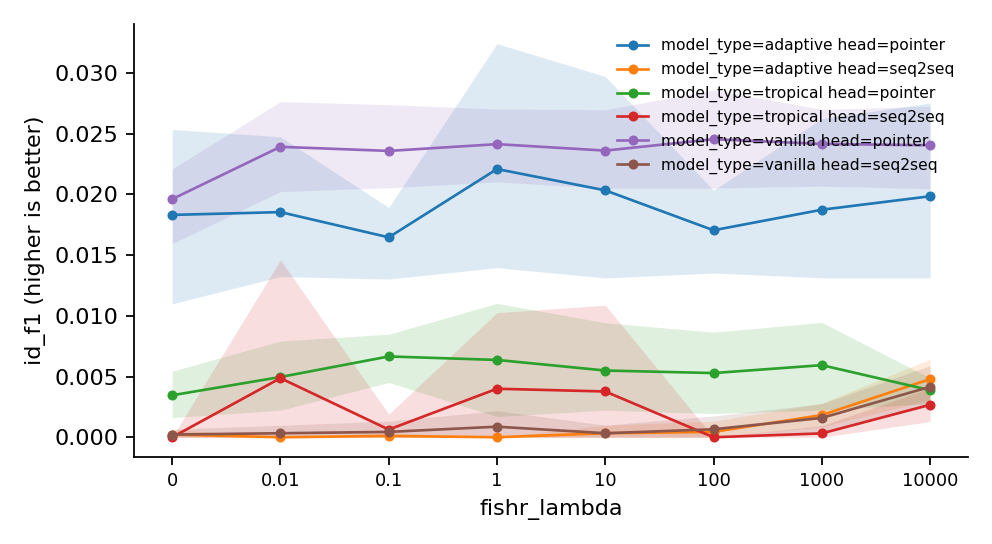
\includegraphics[width=\textwidth]{metric_id_f1.png}
\caption{\texttt{id\_f1} against \texttt{fishr\_lambda}: the mean over seeds with a 95\% bootstrap CI, one line per combination of the other factors.}
\label{fig:id_f1}
\end{figure}

{\small
\begin{longtable}{lllrlrrr}
\caption{\texttt{id\_f1} per cell: mean, 95\% bootstrap CI, SD, seeds, diverged runs.}\label{tab:summary-id_f1}\\
\toprule
\texttt{model\_type} & \texttt{head} & \texttt{fishr\_lambda} & mean & 95\% CI & SD & $n$ & div.\\
\midrule
\endhead
adaptive & pointer & 0 & 0.0183 & [0.011, 0.0253] & 0.00919 & 5 & 0\\
adaptive & pointer & 0.01 & 0.01853 & [0.0132, 0.0247] & 0.00772 & 5 & 0\\
adaptive & pointer & 0.1 & 0.01646 & [0.013, 0.0189] & 0.00381 & 5 & 0\\
adaptive & pointer & 1 & 0.02208 & [0.014, 0.0324] & 0.012 & 5 & 0\\
adaptive & pointer & 10 & 0.02032 & [0.0131, 0.0297] & 0.0111 & 5 & 0\\
adaptive & pointer & 100 & 0.01704 & [0.0135, 0.0203] & 0.0044 & 5 & 0\\
adaptive & pointer & 1000 & 0.01873 & [0.0131, 0.0262] & 0.00879 & 5 & 0\\
adaptive & pointer & 1e+04 & 0.01984 & [0.0131, 0.0275] & 0.00959 & 5 & 0\\
adaptive & seq2seq & 0 & $2.201\times10^{-4}$ & [0, $6.60\times10^{-4}$] & $4.92\times10^{-4}$ & 5 & 0\\
adaptive & seq2seq & 0.01 & 0 & [0, 0] & 0 & 5 & 0\\
adaptive & seq2seq & 0.1 & $1.102\times10^{-4}$ & [0, $3.31\times10^{-4}$] & $2.46\times10^{-4}$ & 5 & 0\\
adaptive & seq2seq & 1 & 0 & [0, 0] & 0 & 5 & 0\\
adaptive & seq2seq & 10 & $3.304\times10^{-4}$ & [0, $9.91\times10^{-4}$] & $7.39\times10^{-4}$ & 5 & 0\\
adaptive & seq2seq & 100 & $4.404\times10^{-4}$ & [0, 0.00132] & $9.85\times10^{-4}$ & 5 & 0\\
adaptive & seq2seq & 1000 & 0.001826 & [$8.42\times10^{-4}$, 0.0028] & 0.0013 & 5 & 0\\
adaptive & seq2seq & 1e+04 & 0.004786 & [0.0031, 0.00643] & 0.00215 & 5 & 0\\
tropical & pointer & 0 & 0.003455 & [0.00161, 0.00544] & 0.00245 & 5 & 0\\
tropical & pointer & 0.01 & 0.00496 & [0.00223, 0.00792] & 0.00355 & 5 & 0\\
tropical & pointer & 0.1 & 0.006651 & [0.00451, 0.00848] & 0.00258 & 5 & 0\\
tropical & pointer & 1 & 0.006365 & [0.00171, 0.011] & 0.00588 & 5 & 0\\
tropical & pointer & 10 & 0.005494 & [0.00223, 0.00942] & 0.00453 & 5 & 0\\
tropical & pointer & 100 & 0.005284 & [0.00195, 0.00865] & 0.00441 & 5 & 0\\
tropical & pointer & 1000 & 0.005935 & [0.00224, 0.00945] & 0.00468 & 5 & 0\\
tropical & pointer & 1e+04 & 0.003875 & [0.00277, 0.00488] & 0.00138 & 5 & 0\\
tropical & seq2seq & 0 & 0 & [0, 0] & 0 & 5 & 0\\
tropical & seq2seq & 0.01 & 0.004865 & [0, 0.0146] & 0.0109 & 5 & 0\\
tropical & seq2seq & 0.1 & $6.327\times10^{-4}$ & [0, 0.0019] & 0.00141 & 5 & 0\\
tropical & seq2seq & 1 & 0.003993 & [0, 0.0103] & 0.00678 & 5 & 0\\
tropical & seq2seq & 10 & 0.003768 & [0, 0.0109] & 0.00784 & 5 & 0\\
tropical & seq2seq & 100 & 0 & [0, 0] & 0 & 5 & 0\\
tropical & seq2seq & 1000 & $3.167\times10^{-4}$ & [0, $9.50\times10^{-4}$] & $7.08\times10^{-4}$ & 5 & 0\\
tropical & seq2seq & 1e+04 & 0.002674 & [0.00129, 0.00405] & 0.00189 & 5 & 0\\
vanilla & pointer & 0 & 0.0196 & [0.0159, 0.0221] & 0.00411 & 5 & 0\\
vanilla & pointer & 0.01 & 0.02391 & [0.0202, 0.0276] & 0.00439 & 5 & 0\\
vanilla & pointer & 0.1 & 0.02357 & [0.0205, 0.0274] & 0.00433 & 5 & 0\\
vanilla & pointer & 1 & 0.02413 & [0.021, 0.027] & 0.00368 & 5 & 0\\
vanilla & pointer & 10 & 0.0236 & [0.0205, 0.027] & 0.00413 & 5 & 0\\
vanilla & pointer & 100 & 0.02454 & [0.0205, 0.0286] & 0.00495 & 5 & 0\\
vanilla & pointer & 1000 & 0.02415 & [0.0207, 0.027] & 0.00397 & 5 & 0\\
vanilla & pointer & 1e+04 & 0.02404 & [0.0205, 0.0272] & 0.00434 & 5 & 0\\
vanilla & seq2seq & 0 & $2.203\times10^{-4}$ & [0, $6.61\times10^{-4}$] & $4.93\times10^{-4}$ & 5 & 0\\
vanilla & seq2seq & 0.01 & $3.302\times10^{-4}$ & [0, $9.91\times10^{-4}$] & $7.38\times10^{-4}$ & 5 & 0\\
vanilla & seq2seq & 0.1 & $4.397\times10^{-4}$ & [0, 0.00132] & $9.83\times10^{-4}$ & 5 & 0\\
vanilla & seq2seq & 1 & $8.704\times10^{-4}$ & [0, 0.00219] & 0.00143 & 5 & 0\\
vanilla & seq2seq & 10 & $3.303\times10^{-4}$ & [0, $9.91\times10^{-4}$] & $7.39\times10^{-4}$ & 5 & 0\\
vanilla & seq2seq & 100 & $6.557\times10^{-4}$ & [0, 0.00176] & 0.00119 & 5 & 0\\
vanilla & seq2seq & 1000 & 0.001592 & [$4.23\times10^{-4}$, 0.00276] & 0.00158 & 5 & 0\\
vanilla & seq2seq & 1e+04 & 0.00415 & [0.00256, 0.0059] & 0.00215 & 5 & 0\\
\bottomrule
\end{longtable}
}

{\small
\begin{longtable}{lllrrrl}
\caption{\texttt{id\_f1}: each level of \texttt{fishr\_lambda} against its control (0), within each combination of the other factors. rank: Wilcoxon signed-rank by seed, Holm.}\label{tab:control-id_f1}\\
\toprule
\texttt{model\_type} & \texttt{head} & \texttt{fishr\_lambda} & difference & 95\% CI & $p$ & \\
\midrule
\endhead
adaptive & pointer & 0.01 & 0.002906 & [-0.00375, 0.004] & 1.0000 & \\
adaptive & pointer & 0.1 & -0.005069 & [-0.00716, 0.00378] & 1.0000 & \\
adaptive & pointer & 1 & 0.003718 & [-0.00156, 0.00938] & 1.0000 & \\
adaptive & pointer & 10 & 0.003214 & [-0.00265, 0.00689] & 1.0000 & \\
adaptive & pointer & 100 & -0.004713 & [-0.00604, 0.00356] & 1.0000 & \\
adaptive & pointer & 1000 & 0.004852 & [-0.0046, 0.00548] & 1.0000 & \\
adaptive & pointer & 1e+04 & 0.004246 & [-0.00313, 0.00531] & 1.0000 & \\
adaptive & seq2seq & 0.01 & 0 & [$-6.60\times10^{-4}$, 0] & 1.0000 & \\
adaptive & seq2seq & 0.1 & 0 & [$-3.30\times10^{-4}$, 0] & 1.0000 & \\
adaptive & seq2seq & 1 & 0 & [$-6.60\times10^{-4}$, 0] & 1.0000 & \\
adaptive & seq2seq & 10 & 0 & [0, $3.31\times10^{-4}$] & 1.0000 & \\
adaptive & seq2seq & 100 & 0 & [0, $6.61\times10^{-4}$] & 1.0000 & \\
adaptive & seq2seq & 1000 & 0.002105 & [$6.56\times10^{-4}$, 0.00236] & 0.7500 & \\
adaptive & seq2seq & 1e+04 & 0.0048 & [0.00309, 0.00603] & 0.4375 & \\
tropical & pointer & 0.01 & $5.295\times10^{-4}$ & [$5.27\times10^{-4}$, 0.00324] & 0.4375 & \\
tropical & pointer & 0.1 & 0.003258 & [0.00255, 0.00388] & 0.4375 & \\
tropical & pointer & 1 & 0.002144 & [$6.17\times10^{-6}$, 0.00581] & 1.0000 & \\
tropical & pointer & 10 & 0.001585 & [$-6.90\times10^{-6}$, 0.00485] & 1.0000 & \\
tropical & pointer & 100 & 0.002143 & [$1.67\times10^{-6}$, 0.00344] & 0.9375 & \\
tropical & pointer & 1000 & 0.002688 & [$5.36\times10^{-4}$, 0.00442] & 1.0000 & \\
tropical & pointer & 1e+04 & $5.536\times10^{-4}$ & [$-8.72\times10^{-4}$, 0.00138] & 1.0000 & \\
tropical & seq2seq & 0.01 & 0 & [0, 0.0146] & 1.0000 & \\
tropical & seq2seq & 0.1 & 0 & [0, 0.0019] & 1.0000 & \\
tropical & seq2seq & 1 & 0 & [0, 0.0103] & 1.0000 & \\
tropical & seq2seq & 10 & 0 & [0, 0.0109] & 1.0000 & \\
tropical & seq2seq & 100 & 0 & [0, 0] & -- & \\
tropical & seq2seq & 1000 & 0 & [0, $9.50\times10^{-4}$] & 1.0000 & \\
tropical & seq2seq & 1e+04 & 0.003262 & [0.00129, 0.00405] & 0.7500 & \\
vanilla & pointer & 0.01 & 0.003695 & [0.00212, 0.00659] & 0.4375 & \\
vanilla & pointer & 0.1 & 0.00313 & [0.00125, 0.00693] & 0.4375 & \\
vanilla & pointer & 1 & 0.004245 & [0.00261, 0.00647] & 0.4375 & \\
vanilla & pointer & 10 & 0.003649 & [0.00178, 0.00627] & 0.4375 & \\
vanilla & pointer & 100 & 0.004802 & [0.00261, 0.00777] & 0.4375 & \\
vanilla & pointer & 1000 & 0.004843 & [0.00261, 0.00614] & 0.4375 & \\
vanilla & pointer & 1e+04 & 0.004641 & [0.00239, 0.00627] & 0.4375 & \\
vanilla & seq2seq & 0.01 & 0 & [0, $3.30\times10^{-4}$] & 1.0000 & \\
vanilla & seq2seq & 0.1 & 0 & [0, $6.58\times10^{-4}$] & 1.0000 & \\
vanilla & seq2seq & 1 & 0 & [0, 0.00151] & 1.0000 & \\
vanilla & seq2seq & 10 & 0 & [0, $3.30\times10^{-4}$] & 1.0000 & \\
vanilla & seq2seq & 100 & 0 & [0, $9.88\times10^{-4}$] & 1.0000 & \\
vanilla & seq2seq & 1000 & 0.002114 & [$-2.20\times10^{-4}$, 0.00276] & 1.0000 & \\
vanilla & seq2seq & 1e+04 & 0.003245 & [0.00256, 0.00568] & 0.4375 & \\
\bottomrule
\end{longtable}
}

{\small
\begin{longtable}{llrrrrr}
\caption{\texttt{id\_f1} against log10 \texttt{fishr\_lambda}: rank: Spearman rho, seed-bootstrap CI, with the Jonckheere--Terpstra ordered-trend $\tau$ and $p$.}\label{tab:trend-id_f1}\\
\toprule
\texttt{model\_type} & \texttt{head} & estimate & 95\% CI & $p$ & JT $\tau$ & JT $p$\\
\midrule
\endhead
adaptive & pointer & -0.01556 & [-0.21, 0.0951] & 0.9293 & -0.019 & 0.8946\\
adaptive & seq2seq & 0.7135 & [0.663, 0.799] & $<10^{-4}$ & 0.484 & 0.0002\\
tropical & pointer & -0.1231 & [-0.24, -0.00556] & 0.4813 & -0.0895 & 0.5151\\
tropical & seq2seq & 0.1606 & [-0.172, 0.538] & 0.3566 & 0.112 & 0.3039\\
vanilla & pointer & 0.1182 & [-0.209, 0.466] & 0.4990 & 0.0857 & 0.5387\\
vanilla & seq2seq & 0.519 & [0.303, 0.793] & 0.0014 & 0.37 & 0.0020\\
\bottomrule
\end{longtable}
}

{\small
\begin{longtable}{lrrrl}
\caption{\texttt{id\_f1}: paired contrasts by seed, Holm-corrected across the cells. rank: Wilcoxon signed-rank by seed, Holm.}\label{tab:paired-id_f1}\\
\toprule
contrast (within) & difference & 95\% CI & $p$ & \\
\midrule
\endhead
\stackcell{model\_type: tropical - vanilla\\\footnotesize head=pointer fishr\_lambda=0 } & -0.01615 & [-0.0206, -0.0117] & 1.0000 & \\
\stackcell{model\_type: tropical - vanilla\\\footnotesize head=pointer fishr\_lambda=0.01 } & -0.01895 & [-0.0253, -0.0126] & 1.0000 & \\
\stackcell{model\_type: tropical - vanilla\\\footnotesize head=pointer fishr\_lambda=0.1 } & -0.01692 & [-0.0222, -0.0116] & 1.0000 & \\
\stackcell{model\_type: tropical - vanilla\\\footnotesize head=pointer fishr\_lambda=1 } & -0.01776 & [-0.0258, -0.00971] & 1.0000 & \\
\stackcell{model\_type: tropical - vanilla\\\footnotesize head=pointer fishr\_lambda=10 } & -0.0181 & [-0.0264, -0.00986] & 1.0000 & \\
\stackcell{model\_type: tropical - vanilla\\\footnotesize head=pointer fishr\_lambda=100 } & -0.01925 & [-0.028, -0.0105] & 1.0000 & \\
\stackcell{model\_type: tropical - vanilla\\\footnotesize head=pointer fishr\_lambda=1000 } & -0.01821 & [-0.0244, -0.0121] & 1.0000 & \\
\stackcell{model\_type: tropical - vanilla\\\footnotesize head=pointer fishr\_lambda=1e+04 } & -0.02016 & [-0.0252, -0.0151] & 1.0000 & \\
\stackcell{model\_type: tropical - vanilla\\\footnotesize head=seq2seq fishr\_lambda=0 } & $-2.203\times10^{-4}$ & [$-8.32\times10^{-4}$, $3.91\times10^{-4}$] & 1.0000 & \\
\stackcell{model\_type: tropical - vanilla\\\footnotesize head=seq2seq fishr\_lambda=0.01 } & 0.004535 & [-0.00923, 0.0183] & 1.0000 & \\
\stackcell{model\_type: tropical - vanilla\\\footnotesize head=seq2seq fishr\_lambda=0.1 } & $1.931\times10^{-4}$ & [-0.00218, 0.00257] & 1.0000 & \\
\stackcell{model\_type: tropical - vanilla\\\footnotesize head=seq2seq fishr\_lambda=1 } & 0.003123 & [-0.00552, 0.0118] & 1.0000 & \\
\stackcell{model\_type: tropical - vanilla\\\footnotesize head=seq2seq fishr\_lambda=10 } & 0.003437 & [-0.00658, 0.0135] & 1.0000 & \\
\stackcell{model\_type: tropical - vanilla\\\footnotesize head=seq2seq fishr\_lambda=100 } & $-6.557\times10^{-4}$ & [-0.00214, $8.25\times10^{-4}$] & 1.0000 & \\
\stackcell{model\_type: tropical - vanilla\\\footnotesize head=seq2seq fishr\_lambda=1000 } & -0.001276 & [-0.00272, $1.71\times10^{-4}$] & 1.0000 & \\
\stackcell{model\_type: tropical - vanilla\\\footnotesize head=seq2seq fishr\_lambda=1e+04 } & -0.001476 & [-0.00376, $8.11\times10^{-4}$] & 1.0000 & \\
\stackcell{model\_type: adaptive - vanilla\\\footnotesize head=pointer fishr\_lambda=0 } & -0.001301 & [-0.0151, 0.0125] & 1.0000 & \\
\stackcell{model\_type: adaptive - vanilla\\\footnotesize head=pointer fishr\_lambda=0.01 } & -0.005375 & [-0.012, 0.00127] & 1.0000 & \\
\stackcell{model\_type: adaptive - vanilla\\\footnotesize head=pointer fishr\_lambda=0.1 } & -0.007114 & [-0.0133, $-9.30\times10^{-4}$] & 1.0000 & \\
\stackcell{model\_type: adaptive - vanilla\\\footnotesize head=pointer fishr\_lambda=1 } & -0.002048 & [-0.0141, 0.00996] & 1.0000 & \\
\stackcell{model\_type: adaptive - vanilla\\\footnotesize head=pointer fishr\_lambda=10 } & -0.003273 & [-0.0137, 0.00717] & 1.0000 & \\
\stackcell{model\_type: adaptive - vanilla\\\footnotesize head=pointer fishr\_lambda=100 } & -0.007496 & [-0.0131, -0.00185] & 1.0000 & \\
\stackcell{model\_type: adaptive - vanilla\\\footnotesize head=pointer fishr\_lambda=1000 } & -0.005417 & [-0.0137, 0.00288] & 1.0000 & \\
\stackcell{model\_type: adaptive - vanilla\\\footnotesize head=pointer fishr\_lambda=1e+04 } & -0.004197 & [-0.014, 0.00564] & 1.0000 & \\
\stackcell{model\_type: adaptive - vanilla\\\footnotesize head=seq2seq fishr\_lambda=0 } & $-1.212\times10^{-7}$ & [$-4.58\times10^{-7}$, $2.15\times10^{-7}$] & 1.0000 & \\
\stackcell{model\_type: adaptive - vanilla\\\footnotesize head=seq2seq fishr\_lambda=0.01 } & $-3.302\times10^{-4}$ & [-0.00125, $5.87\times10^{-4}$] & 1.0000 & \\
\stackcell{model\_type: adaptive - vanilla\\\footnotesize head=seq2seq fishr\_lambda=0.1 } & $-3.295\times10^{-4}$ & [-0.00124, $5.85\times10^{-4}$] & 1.0000 & \\
\stackcell{model\_type: adaptive - vanilla\\\footnotesize head=seq2seq fishr\_lambda=1 } & $-8.704\times10^{-4}$ & [-0.00265, $9.06\times10^{-4}$] & 1.0000 & \\
\stackcell{model\_type: adaptive - vanilla\\\footnotesize head=seq2seq fishr\_lambda=10 } & $9.094\times10^{-8}$ & [$-1.62\times10^{-7}$, $3.43\times10^{-7}$] & 1.0000 & \\
\stackcell{model\_type: adaptive - vanilla\\\footnotesize head=seq2seq fishr\_lambda=100 } & $-2.153\times10^{-4}$ & [$-5.81\times10^{-4}$, $1.51\times10^{-4}$] & 1.0000 & \\
\stackcell{model\_type: adaptive - vanilla\\\footnotesize head=seq2seq fishr\_lambda=1000 } & $2.331\times10^{-4}$ & [-0.00213, 0.0026] & 1.0000 & \\
\stackcell{model\_type: adaptive - vanilla\\\footnotesize head=seq2seq fishr\_lambda=1e+04 } & $6.362\times10^{-4}$ & [$-2.23\times10^{-4}$, 0.0015] & 1.0000 & \\
\stackcell{head: pointer - seq2seq\\\footnotesize model\_type=adaptive fishr\_lambda=0 } & 0.01808 & [0.00642, 0.0297] & 1.0000 & \\
\stackcell{head: pointer - seq2seq\\\footnotesize model\_type=adaptive fishr\_lambda=0.01 } & 0.01853 & [0.00894, 0.0281] & 1.0000 & \\
\stackcell{head: pointer - seq2seq\\\footnotesize model\_type=adaptive fishr\_lambda=0.1 } & 0.01635 & [0.0117, 0.021] & 1.0000 & \\
\stackcell{head: pointer - seq2seq\\\footnotesize model\_type=adaptive fishr\_lambda=1 } & 0.02208 & [0.00724, 0.0369] & 1.0000 & \\
\stackcell{head: pointer - seq2seq\\\footnotesize model\_type=adaptive fishr\_lambda=10 } & 0.01999 & [0.0059, 0.0341] & 1.0000 & \\
\stackcell{head: pointer - seq2seq\\\footnotesize model\_type=adaptive fishr\_lambda=100 } & 0.0166 & [0.0112, 0.022] & 1.0000 & \\
\stackcell{head: pointer - seq2seq\\\footnotesize model\_type=adaptive fishr\_lambda=1000 } & 0.0169 & [0.00626, 0.0275] & 1.0000 & \\
\stackcell{head: pointer - seq2seq\\\footnotesize model\_type=adaptive fishr\_lambda=1e+04 } & 0.01505 & [0.00383, 0.0263] & 1.0000 & \\
\stackcell{head: pointer - seq2seq\\\footnotesize model\_type=tropical fishr\_lambda=0 } & 0.003455 & [$4.10\times10^{-4}$, 0.0065] & 1.0000 & \\
\stackcell{head: pointer - seq2seq\\\footnotesize model\_type=tropical fishr\_lambda=0.01 } & $9.427\times10^{-5}$ & [-0.0156, 0.0158] & 1.0000 & \\
\stackcell{head: pointer - seq2seq\\\footnotesize model\_type=tropical fishr\_lambda=0.1 } & 0.006019 & [0.00224, 0.00979] & 1.0000 & \\
\stackcell{head: pointer - seq2seq\\\footnotesize model\_type=tropical fishr\_lambda=1 } & 0.002372 & [-0.0112, 0.016] & 1.0000 & \\
\stackcell{head: pointer - seq2seq\\\footnotesize model\_type=tropical fishr\_lambda=10 } & 0.001726 & [-0.0115, 0.015] & 1.0000 & \\
\stackcell{head: pointer - seq2seq\\\footnotesize model\_type=tropical fishr\_lambda=100 } & 0.005284 & [$-1.94\times10^{-4}$, 0.0108] & 1.0000 & \\
\stackcell{head: pointer - seq2seq\\\footnotesize model\_type=tropical fishr\_lambda=1000 } & 0.005618 & [$-6.48\times10^{-4}$, 0.0119] & 1.0000 & \\
\stackcell{head: pointer - seq2seq\\\footnotesize model\_type=tropical fishr\_lambda=1e+04 } & 0.0012 & [$-9.01\times10^{-4}$, 0.0033] & 1.0000 & \\
\stackcell{head: pointer - seq2seq\\\footnotesize model\_type=vanilla fishr\_lambda=0 } & 0.01938 & [0.0143, 0.0245] & 1.0000 & \\
\stackcell{head: pointer - seq2seq\\\footnotesize model\_type=vanilla fishr\_lambda=0.01 } & 0.02358 & [0.0181, 0.0291] & 1.0000 & \\
\stackcell{head: pointer - seq2seq\\\footnotesize model\_type=vanilla fishr\_lambda=0.1 } & 0.02313 & [0.0174, 0.0289] & 1.0000 & \\
\stackcell{head: pointer - seq2seq\\\footnotesize model\_type=vanilla fishr\_lambda=1 } & 0.02326 & [0.019, 0.0276] & 1.0000 & \\
\stackcell{head: pointer - seq2seq\\\footnotesize model\_type=vanilla fishr\_lambda=10 } & 0.02327 & [0.0179, 0.0287] & 1.0000 & \\
\stackcell{head: pointer - seq2seq\\\footnotesize model\_type=vanilla fishr\_lambda=100 } & 0.02388 & [0.0175, 0.0303] & 1.0000 & \\
\stackcell{head: pointer - seq2seq\\\footnotesize model\_type=vanilla fishr\_lambda=1000 } & 0.02255 & [0.0176, 0.0275] & 1.0000 & \\
\stackcell{head: pointer - seq2seq\\\footnotesize model\_type=vanilla fishr\_lambda=1e+04 } & 0.01989 & [0.0169, 0.0229] & 1.0000 & \\
\bottomrule
\end{longtable}
}

\subsection{\texttt{id\_exact}}
\begin{figure}[tbp]
\centering
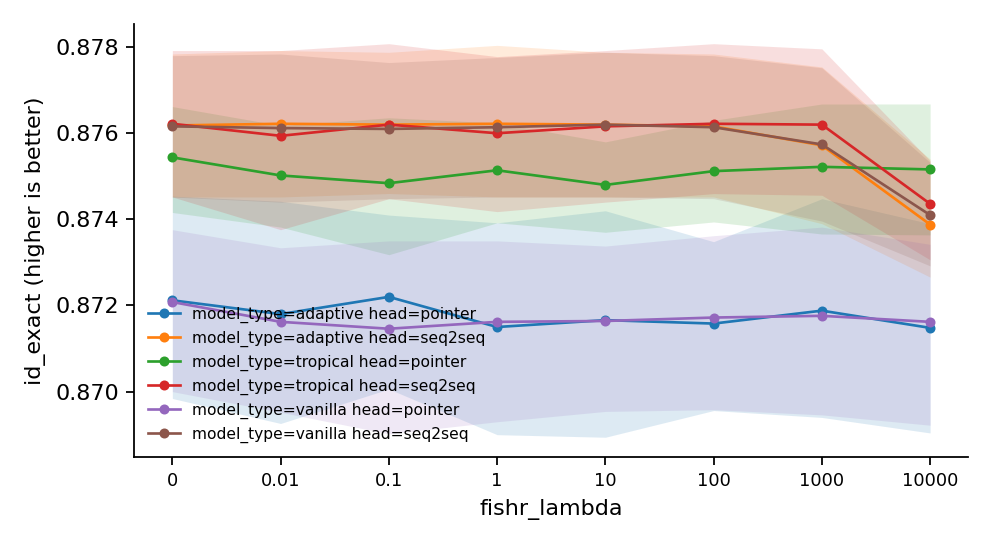
\includegraphics[width=\textwidth]{metric_id_exact.png}
\caption{\texttt{id\_exact} against \texttt{fishr\_lambda}: the mean over seeds with a 95\% bootstrap CI, one line per combination of the other factors.}
\label{fig:id_exact}
\end{figure}

{\small
\begin{longtable}{lllrlrrr}
\caption{\texttt{id\_exact} per cell: mean, 95\% bootstrap CI, SD, seeds, diverged runs.}\label{tab:summary-id_exact}\\
\toprule
\texttt{model\_type} & \texttt{head} & \texttt{fishr\_lambda} & mean & 95\% CI & SD & $n$ & div.\\
\midrule
\endhead
adaptive & pointer & 0 & 0.8721 & [0.87, 0.875] & 0.0031 & 5 & 0\\
adaptive & pointer & 0.01 & 0.8718 & [0.869, 0.874] & 0.00332 & 5 & 0\\
adaptive & pointer & 0.1 & 0.8722 & [0.87, 0.874] & 0.00278 & 5 & 0\\
adaptive & pointer & 1 & 0.8715 & [0.869, 0.874] & 0.00331 & 5 & 0\\
adaptive & pointer & 10 & 0.8717 & [0.869, 0.874] & 0.00341 & 5 & 0\\
adaptive & pointer & 100 & 0.8716 & [0.87, 0.873] & 0.00261 & 5 & 0\\
adaptive & pointer & 1000 & 0.8719 & [0.869, 0.874] & 0.00338 & 5 & 0\\
adaptive & pointer & 1e+04 & 0.8715 & [0.869, 0.874] & 0.00328 & 5 & 0\\
adaptive & seq2seq & 0 & 0.8762 & [0.875, 0.878] & 0.00216 & 5 & 0\\
adaptive & seq2seq & 0.01 & 0.8762 & [0.875, 0.878] & 0.00222 & 5 & 0\\
adaptive & seq2seq & 0.1 & 0.8762 & [0.875, 0.878] & 0.00219 & 5 & 0\\
adaptive & seq2seq & 1 & 0.8762 & [0.875, 0.878] & 0.00222 & 5 & 0\\
adaptive & seq2seq & 10 & 0.8762 & [0.875, 0.878] & 0.00219 & 5 & 0\\
adaptive & seq2seq & 100 & 0.8762 & [0.875, 0.878] & 0.00218 & 5 & 0\\
adaptive & seq2seq & 1000 & 0.8757 & [0.874, 0.878] & 0.00241 & 5 & 0\\
adaptive & seq2seq & 1e+04 & 0.8739 & [0.873, 0.875] & 0.00172 & 5 & 0\\
tropical & pointer & 0 & 0.8754 & [0.874, 0.877] & 0.0016 & 5 & 0\\
tropical & pointer & 0.01 & 0.875 & [0.874, 0.876] & 0.00152 & 5 & 0\\
tropical & pointer & 0.1 & 0.8748 & [0.873, 0.876] & 0.00202 & 5 & 0\\
tropical & pointer & 1 & 0.8751 & [0.874, 0.876] & 0.00147 & 5 & 0\\
tropical & pointer & 10 & 0.8748 & [0.874, 0.876] & 0.00135 & 5 & 0\\
tropical & pointer & 100 & 0.8751 & [0.874, 0.876] & 0.00157 & 5 & 0\\
tropical & pointer & 1000 & 0.8752 & [0.874, 0.877] & 0.00194 & 5 & 0\\
tropical & pointer & 1e+04 & 0.8752 & [0.874, 0.877] & 0.00201 & 5 & 0\\
tropical & seq2seq & 0 & 0.8762 & [0.875, 0.878] & 0.00222 & 5 & 0\\
tropical & seq2seq & 0.01 & 0.8759 & [0.874, 0.878] & 0.00265 & 5 & 0\\
tropical & seq2seq & 0.1 & 0.8762 & [0.874, 0.878] & 0.00225 & 5 & 0\\
tropical & seq2seq & 1 & 0.876 & [0.874, 0.878] & 0.00238 & 5 & 0\\
tropical & seq2seq & 10 & 0.8762 & [0.874, 0.878] & 0.00231 & 5 & 0\\
tropical & seq2seq & 100 & 0.8762 & [0.875, 0.878] & 0.00222 & 5 & 0\\
tropical & seq2seq & 1000 & 0.8762 & [0.875, 0.878] & 0.00217 & 5 & 0\\
tropical & seq2seq & 1e+04 & 0.8744 & [0.873, 0.875] & 0.00149 & 5 & 0\\
vanilla & pointer & 0 & 0.8721 & [0.87, 0.874] & 0.00246 & 5 & 0\\
vanilla & pointer & 0.01 & 0.8716 & [0.87, 0.873] & 0.00254 & 5 & 0\\
vanilla & pointer & 0.1 & 0.8715 & [0.869, 0.874] & 0.00289 & 5 & 0\\
vanilla & pointer & 1 & 0.8716 & [0.869, 0.873] & 0.0027 & 5 & 0\\
vanilla & pointer & 10 & 0.8716 & [0.87, 0.873] & 0.00248 & 5 & 0\\
vanilla & pointer & 100 & 0.8717 & [0.87, 0.874] & 0.00271 & 5 & 0\\
vanilla & pointer & 1000 & 0.8718 & [0.869, 0.874] & 0.0029 & 5 & 0\\
vanilla & pointer & 1e+04 & 0.8716 & [0.869, 0.873] & 0.0027 & 5 & 0\\
vanilla & seq2seq & 0 & 0.8762 & [0.875, 0.878] & 0.00213 & 5 & 0\\
vanilla & seq2seq & 0.01 & 0.8761 & [0.874, 0.878] & 0.00224 & 5 & 0\\
vanilla & seq2seq & 0.1 & 0.8761 & [0.874, 0.878] & 0.0021 & 5 & 0\\
vanilla & seq2seq & 1 & 0.8761 & [0.875, 0.878] & 0.0021 & 5 & 0\\
vanilla & seq2seq & 10 & 0.8762 & [0.875, 0.878] & 0.00219 & 5 & 0\\
vanilla & seq2seq & 100 & 0.8761 & [0.874, 0.878] & 0.00215 & 5 & 0\\
vanilla & seq2seq & 1000 & 0.8757 & [0.874, 0.878] & 0.00237 & 5 & 0\\
vanilla & seq2seq & 1e+04 & 0.8741 & [0.873, 0.875] & 0.00166 & 5 & 0\\
\bottomrule
\end{longtable}
}

{\small
\begin{longtable}{lllrrrl}
\caption{\texttt{id\_exact}: each level of \texttt{fishr\_lambda} against its control (0), within each combination of the other factors. parametric: Dunnett vs control.}\label{tab:control-id_exact}\\
\toprule
\texttt{model\_type} & \texttt{head} & \texttt{fishr\_lambda} & difference & 95\% CI & $p$ & \\
\midrule
\endhead
adaptive & pointer & 0.01 & $-3.200\times10^{-4}$ & [-0.00584, 0.0052] & 1.0000 & \\
adaptive & pointer & 0.1 & $8.000\times10^{-5}$ & [-0.00544, 0.0056] & 1.0000 & \\
adaptive & pointer & 1 & $-6.200\times10^{-4}$ & [-0.00614, 0.0049] & 0.9998 & \\
adaptive & pointer & 10 & $-4.600\times10^{-4}$ & [-0.00598, 0.00506] & 1.0000 & \\
adaptive & pointer & 100 & $-5.400\times10^{-4}$ & [-0.00606, 0.00498] & 0.9999 & \\
adaptive & pointer & 1000 & $-2.400\times10^{-4}$ & [-0.00576, 0.00528] & 1.0000 & \\
adaptive & pointer & 1e+04 & $-6.400\times10^{-4}$ & [-0.00616, 0.00488] & 0.9997 & \\
adaptive & seq2seq & 0.01 & $4.000\times10^{-5}$ & [-0.00375, 0.00383] & 1.0000 & \\
adaptive & seq2seq & 0.1 & $2.000\times10^{-5}$ & [-0.00377, 0.00381] & 1.0000 & \\
adaptive & seq2seq & 1 & $4.000\times10^{-5}$ & [-0.00375, 0.00383] & 1.0000 & \\
adaptive & seq2seq & 10 & $2.000\times10^{-5}$ & [-0.00377, 0.00381] & 1.0000 & \\
adaptive & seq2seq & 100 & $-2.000\times10^{-5}$ & [-0.00381, 0.00377] & 1.0000 & \\
adaptive & seq2seq & 1000 & $-4.600\times10^{-4}$ & [-0.00425, 0.00333] & 0.9996 & \\
adaptive & seq2seq & 1e+04 & -0.0023 & [-0.00609, 0.00149] & 0.4043 & \\
tropical & pointer & 0.01 & $-4.200\times10^{-4}$ & [-0.0034, 0.00256] & 0.9990 & \\
tropical & pointer & 0.1 & $-6.000\times10^{-4}$ & [-0.00358, 0.00238] & 0.9913 & \\
tropical & pointer & 1 & $-3.000\times10^{-4}$ & [-0.00328, 0.00268] & 0.9999 & \\
tropical & pointer & 10 & $-6.400\times10^{-4}$ & [-0.00362, 0.00234] & 0.9876 & \\
tropical & pointer & 100 & $-3.200\times10^{-4}$ & [-0.0033, 0.00266] & 0.9998 & \\
tropical & pointer & 1000 & $-2.200\times10^{-4}$ & [-0.0032, 0.00276] & 1.0000 & \\
tropical & pointer & 1e+04 & $-2.800\times10^{-4}$ & [-0.00326, 0.0027] & 0.9999 & \\
tropical & seq2seq & 0.01 & $-2.800\times10^{-4}$ & [-0.00418, 0.00362] & 1.0000 & \\
tropical & seq2seq & 0.1 & $-2.000\times10^{-5}$ & [-0.00392, 0.00388] & 1.0000 & \\
tropical & seq2seq & 1 & $-2.200\times10^{-4}$ & [-0.00412, 0.00368] & 1.0000 & \\
tropical & seq2seq & 10 & $-6.000\times10^{-5}$ & [-0.00396, 0.00384] & 1.0000 & \\
tropical & seq2seq & 100 & 0 & [-0.0039, 0.0039] & 1.0000 & \\
tropical & seq2seq & 1000 & $-2.000\times10^{-5}$ & [-0.00392, 0.00388] & 1.0000 & \\
tropical & seq2seq & 1e+04 & -0.00186 & [-0.00576, 0.00204] & 0.6470 & \\
vanilla & pointer & 0.01 & $-4.600\times10^{-4}$ & [-0.00514, 0.00422] & 0.9999 & \\
vanilla & pointer & 0.1 & $-6.200\times10^{-4}$ & [-0.0053, 0.00406] & 0.9993 & \\
vanilla & pointer & 1 & $-4.600\times10^{-4}$ & [-0.00514, 0.00422] & 0.9999 & \\
vanilla & pointer & 10 & $-4.400\times10^{-4}$ & [-0.00512, 0.00424] & 0.9999 & \\
vanilla & pointer & 100 & $-3.600\times10^{-4}$ & [-0.00504, 0.00432] & 1.0000 & \\
vanilla & pointer & 1000 & $-3.200\times10^{-4}$ & [-0.005, 0.00436] & 1.0000 & \\
vanilla & pointer & 1e+04 & $-4.600\times10^{-4}$ & [-0.00514, 0.00422] & 0.9999 & \\
vanilla & seq2seq & 0.01 & $-4.000\times10^{-5}$ & [-0.00375, 0.00367] & 1.0000 & \\
vanilla & seq2seq & 0.1 & $-6.000\times10^{-5}$ & [-0.00377, 0.00365] & 1.0000 & \\
vanilla & seq2seq & 1 & $-2.000\times10^{-5}$ & [-0.00373, 0.00369] & 1.0000 & \\
vanilla & seq2seq & 10 & $4.000\times10^{-5}$ & [-0.00367, 0.00375] & 1.0000 & \\
vanilla & seq2seq & 100 & $-2.000\times10^{-5}$ & [-0.00373, 0.00369] & 1.0000 & \\
vanilla & seq2seq & 1000 & $-4.200\times10^{-4}$ & [-0.00413, 0.00329] & 0.9998 & \\
vanilla & seq2seq & 1e+04 & -0.00206 & [-0.00577, 0.00165] & 0.4960 & \\
\bottomrule
\end{longtable}
}

{\small
\begin{longtable}{llrrrrr}
\caption{\texttt{id\_exact} against log10 \texttt{fishr\_lambda}: parametric: OLS slope t-test, seed-bootstrap CI, with the Jonckheere--Terpstra ordered-trend $\tau$ and $p$.}\label{tab:trend-id_exact}\\
\toprule
\texttt{model\_type} & \texttt{head} & estimate & 95\% CI & $p$ & JT $\tau$ & JT $p$\\
\midrule
\endhead
adaptive & pointer & $-5.429\times10^{-5}$ & [$-1.08\times10^{-4}$, $-1.29\times10^{-5}$] & 0.8276 & -0.0324 & 0.8084\\
adaptive & seq2seq & $-2.871\times10^{-4}$ & [$-4.08\times10^{-4}$, $-1.92\times10^{-4}$] & 0.1121 & -0.253 & 0.0542\\
tropical & pointer & $4.143\times10^{-5}$ & [$-4.07\times10^{-5}$, $1.51\times10^{-4}$] & 0.7594 & 0.021 & 0.8832\\
tropical & seq2seq & $-1.614\times10^{-4}$ & [$-2.89\times10^{-4}$, $-3.36\times10^{-5}$] & 0.3766 & -0.112 & 0.3903\\
vanilla & pointer & $2.500\times10^{-5}$ & [$-1.71\times10^{-5}$, $7.07\times10^{-5}$] & 0.9064 & 0.00952 & 0.9498\\
vanilla & seq2seq & $-2.421\times10^{-4}$ & [$-3.44\times10^{-4}$, $-1.53\times10^{-4}$] & 0.1668 & -0.211 & 0.1186\\
\bottomrule
\end{longtable}
}

{\small
\begin{longtable}{lrrrl}
\caption{\texttt{id\_exact}: paired contrasts by seed, Holm-corrected across the cells. parametric: paired t-test by seed, Holm.}\label{tab:paired-id_exact}\\
\toprule
contrast (within) & difference & 95\% CI & $p$ & \\
\midrule
\endhead
\stackcell{model\_type: tropical - vanilla\\\footnotesize head=pointer fishr\_lambda=0 } & 0.00336 & [0.00196, 0.00476] & 0.0373 & *\\
\stackcell{model\_type: tropical - vanilla\\\footnotesize head=pointer fishr\_lambda=0.01 } & 0.0034 & [0.00194, 0.00486] & 0.0384 & *\\
\stackcell{model\_type: tropical - vanilla\\\footnotesize head=pointer fishr\_lambda=0.1 } & 0.00338 & [0.00215, 0.00461] & 0.0251 & *\\
\stackcell{model\_type: tropical - vanilla\\\footnotesize head=pointer fishr\_lambda=1 } & 0.00352 & [0.00179, 0.00525] & 0.0532 & \\
\stackcell{model\_type: tropical - vanilla\\\footnotesize head=pointer fishr\_lambda=10 } & 0.00316 & [0.00146, 0.00486] & 0.0668 & \\
\stackcell{model\_type: tropical - vanilla\\\footnotesize head=pointer fishr\_lambda=100 } & 0.0034 & [0.0014, 0.0054] & 0.0829 & \\
\stackcell{model\_type: tropical - vanilla\\\footnotesize head=pointer fishr\_lambda=1000 } & 0.00346 & [0.00184, 0.00508] & 0.0487 & *\\
\stackcell{model\_type: tropical - vanilla\\\footnotesize head=pointer fishr\_lambda=1e+04 } & 0.00354 & [0.00214, 0.00494] & 0.0328 & *\\
\stackcell{model\_type: tropical - vanilla\\\footnotesize head=seq2seq fishr\_lambda=0 } & $6.000\times10^{-5}$ & [$-1.07\times10^{-4}$, $2.27\times10^{-4}$] & 1.0000 & \\
\stackcell{model\_type: tropical - vanilla\\\footnotesize head=seq2seq fishr\_lambda=0.01 } & $-1.800\times10^{-4}$ & [$-8.28\times10^{-4}$, $4.68\times10^{-4}$] & 1.0000 & \\
\stackcell{model\_type: tropical - vanilla\\\footnotesize head=seq2seq fishr\_lambda=0.1 } & $1.000\times10^{-4}$ & [$-1.78\times10^{-4}$, $3.78\times10^{-4}$] & 1.0000 & \\
\stackcell{model\_type: tropical - vanilla\\\footnotesize head=seq2seq fishr\_lambda=1 } & $-1.400\times10^{-4}$ & [$-6.49\times10^{-4}$, $3.69\times10^{-4}$] & 1.0000 & \\
\stackcell{model\_type: tropical - vanilla\\\footnotesize head=seq2seq fishr\_lambda=10 } & $-4.000\times10^{-5}$ & [$-2.28\times10^{-4}$, $1.48\times10^{-4}$] & 1.0000 & \\
\stackcell{model\_type: tropical - vanilla\\\footnotesize head=seq2seq fishr\_lambda=100 } & $8.000\times10^{-5}$ & [$-8.19\times10^{-5}$, $2.42\times10^{-4}$] & 1.0000 & \\
\stackcell{model\_type: tropical - vanilla\\\footnotesize head=seq2seq fishr\_lambda=1000 } & $4.600\times10^{-4}$ & [$1.74\times10^{-4}$, $7.46\times10^{-4}$] & 0.0887 & \\
\stackcell{model\_type: tropical - vanilla\\\footnotesize head=seq2seq fishr\_lambda=1e+04 } & $2.600\times10^{-4}$ & [-0.00131, 0.00183] & 1.0000 & \\
\stackcell{model\_type: adaptive - vanilla\\\footnotesize head=pointer fishr\_lambda=0 } & $4.000\times10^{-5}$ & [-0.00248, 0.00256] & 1.0000 & \\
\stackcell{model\_type: adaptive - vanilla\\\footnotesize head=pointer fishr\_lambda=0.01 } & $1.800\times10^{-4}$ & [-0.00191, 0.00227] & 1.0000 & \\
\stackcell{model\_type: adaptive - vanilla\\\footnotesize head=pointer fishr\_lambda=0.1 } & $7.400\times10^{-4}$ & [$-4.91\times10^{-4}$, 0.00197] & 1.0000 & \\
\stackcell{model\_type: adaptive - vanilla\\\footnotesize head=pointer fishr\_lambda=1 } & $-1.200\times10^{-4}$ & [-0.00225, 0.00201] & 1.0000 & \\
\stackcell{model\_type: adaptive - vanilla\\\footnotesize head=pointer fishr\_lambda=10 } & $2.000\times10^{-5}$ & [-0.00199, 0.00203] & 1.0000 & \\
\stackcell{model\_type: adaptive - vanilla\\\footnotesize head=pointer fishr\_lambda=100 } & $-1.400\times10^{-4}$ & [-0.00191, 0.00163] & 1.0000 & \\
\stackcell{model\_type: adaptive - vanilla\\\footnotesize head=pointer fishr\_lambda=1000 } & $1.200\times10^{-4}$ & [-0.00158, 0.00182] & 1.0000 & \\
\stackcell{model\_type: adaptive - vanilla\\\footnotesize head=pointer fishr\_lambda=1e+04 } & $-1.400\times10^{-4}$ & [-0.00222, 0.00194] & 1.0000 & \\
\stackcell{model\_type: adaptive - vanilla\\\footnotesize head=seq2seq fishr\_lambda=0 } & $2.000\times10^{-5}$ & [$-3.55\times10^{-5}$, $7.55\times10^{-5}$] & 1.0000 & \\
\stackcell{model\_type: adaptive - vanilla\\\footnotesize head=seq2seq fishr\_lambda=0.01 } & $1.000\times10^{-4}$ & [$-7.56\times10^{-5}$, $2.76\times10^{-4}$] & 1.0000 & \\
\stackcell{model\_type: adaptive - vanilla\\\footnotesize head=seq2seq fishr\_lambda=0.1 } & $1.000\times10^{-4}$ & [$-1.15\times10^{-4}$, $3.15\times10^{-4}$] & 1.0000 & \\
\stackcell{model\_type: adaptive - vanilla\\\footnotesize head=seq2seq fishr\_lambda=1 } & $8.000\times10^{-5}$ & [$-1.42\times10^{-4}$, $3.02\times10^{-4}$] & 1.0000 & \\
\stackcell{model\_type: adaptive - vanilla\\\footnotesize head=seq2seq fishr\_lambda=10 } & 0 & [--, --] & -- & \\
\stackcell{model\_type: adaptive - vanilla\\\footnotesize head=seq2seq fishr\_lambda=100 } & $2.000\times10^{-5}$ & [$-3.55\times10^{-5}$, $7.55\times10^{-5}$] & 1.0000 & \\
\stackcell{model\_type: adaptive - vanilla\\\footnotesize head=seq2seq fishr\_lambda=1000 } & $-2.000\times10^{-5}$ & [$-1.82\times10^{-4}$, $1.42\times10^{-4}$] & 1.0000 & \\
\stackcell{model\_type: adaptive - vanilla\\\footnotesize head=seq2seq fishr\_lambda=1e+04 } & $-2.200\times10^{-4}$ & [$-6.62\times10^{-4}$, $2.22\times10^{-4}$] & 1.0000 & \\
\stackcell{head: pointer - seq2seq\\\footnotesize model\_type=adaptive fishr\_lambda=0 } & -0.00406 & [-0.00584, -0.00228] & 0.0481 & *\\
\stackcell{head: pointer - seq2seq\\\footnotesize model\_type=adaptive fishr\_lambda=0.01 } & -0.00442 & [-0.00648, -0.00236] & 0.0556 & \\
\stackcell{head: pointer - seq2seq\\\footnotesize model\_type=adaptive fishr\_lambda=0.1 } & -0.004 & [-0.00533, -0.00267] & 0.0235 & *\\
\stackcell{head: pointer - seq2seq\\\footnotesize model\_type=adaptive fishr\_lambda=1 } & -0.00472 & [-0.00709, -0.00235] & 0.0608 & \\
\stackcell{head: pointer - seq2seq\\\footnotesize model\_type=adaptive fishr\_lambda=10 } & -0.00454 & [-0.00676, -0.00232] & 0.0608 & \\
\stackcell{head: pointer - seq2seq\\\footnotesize model\_type=adaptive fishr\_lambda=100 } & -0.00458 & [-0.00625, -0.00291] & 0.0285 & *\\
\stackcell{head: pointer - seq2seq\\\footnotesize model\_type=adaptive fishr\_lambda=1000 } & -0.00384 & [-0.00571, -0.00197] & 0.0608 & \\
\stackcell{head: pointer - seq2seq\\\footnotesize model\_type=adaptive fishr\_lambda=1e+04 } & -0.0024 & [-0.00599, 0.00119] & 0.5285 & \\
\stackcell{head: pointer - seq2seq\\\footnotesize model\_type=tropical fishr\_lambda=0 } & $-7.800\times10^{-4}$ & [-0.00182, $2.57\times10^{-4}$] & 0.5247 & \\
\stackcell{head: pointer - seq2seq\\\footnotesize model\_type=tropical fishr\_lambda=0.01 } & $-9.200\times10^{-4}$ & [-0.0026, $7.63\times10^{-4}$] & 0.5285 & \\
\stackcell{head: pointer - seq2seq\\\footnotesize model\_type=tropical fishr\_lambda=0.1 } & -0.00136 & [-0.00221, $-5.06\times10^{-4}$] & 0.1150 & \\
\stackcell{head: pointer - seq2seq\\\footnotesize model\_type=tropical fishr\_lambda=1 } & $-8.600\times10^{-4}$ & [-0.00213, $4.05\times10^{-4}$] & 0.5285 & \\
\stackcell{head: pointer - seq2seq\\\footnotesize model\_type=tropical fishr\_lambda=10 } & -0.00136 & [-0.00295, $2.29\times10^{-4}$] & 0.4579 & \\
\stackcell{head: pointer - seq2seq\\\footnotesize model\_type=tropical fishr\_lambda=100 } & -0.0011 & [-0.00211, $-9.13\times10^{-5}$] & 0.2721 & \\
\stackcell{head: pointer - seq2seq\\\footnotesize model\_type=tropical fishr\_lambda=1000 } & $-9.800\times10^{-4}$ & [-0.00177, $-1.88\times10^{-4}$] & 0.2335 & \\
\stackcell{head: pointer - seq2seq\\\footnotesize model\_type=tropical fishr\_lambda=1e+04 } & $8.000\times10^{-4}$ & [$-6.24\times10^{-4}$, 0.00222] & 0.5285 & \\
\stackcell{head: pointer - seq2seq\\\footnotesize model\_type=vanilla fishr\_lambda=0 } & -0.00408 & [-0.00558, -0.00258] & 0.0285 & *\\
\stackcell{head: pointer - seq2seq\\\footnotesize model\_type=vanilla fishr\_lambda=0.01 } & -0.0045 & [-0.00574, -0.00326] & 0.0130 & *\\
\stackcell{head: pointer - seq2seq\\\footnotesize model\_type=vanilla fishr\_lambda=0.1 } & -0.00464 & [-0.00623, -0.00305] & 0.0239 & *\\
\stackcell{head: pointer - seq2seq\\\footnotesize model\_type=vanilla fishr\_lambda=1 } & -0.00452 & [-0.00604, -0.003] & 0.0236 & *\\
\stackcell{head: pointer - seq2seq\\\footnotesize model\_type=vanilla fishr\_lambda=10 } & -0.00456 & [-0.00593, -0.00319] & 0.0175 & *\\
\stackcell{head: pointer - seq2seq\\\footnotesize model\_type=vanilla fishr\_lambda=100 } & -0.00442 & [-0.00584, -0.003] & 0.0217 & *\\
\stackcell{head: pointer - seq2seq\\\footnotesize model\_type=vanilla fishr\_lambda=1000 } & -0.00398 & [-0.00551, -0.00245] & 0.0315 & *\\
\stackcell{head: pointer - seq2seq\\\footnotesize model\_type=vanilla fishr\_lambda=1e+04 } & -0.00248 & [-0.00447, $-4.87\times10^{-4}$] & 0.2335 & \\
\bottomrule
\end{longtable}
}


\section{Curves}
\begin{figure}[tbp]
\centering
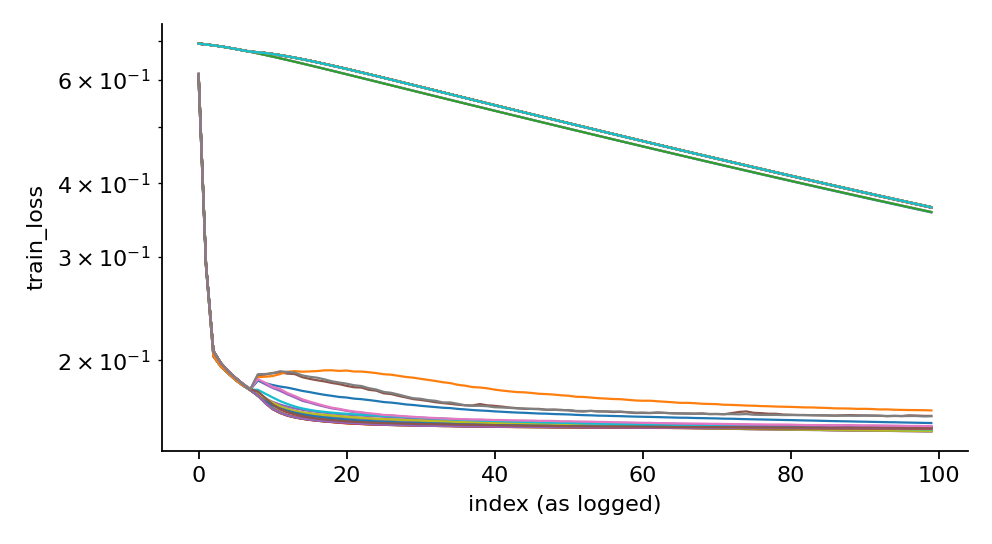
\includegraphics[width=\textwidth]{curve_train_loss.png}
\caption{\texttt{train\_loss}, the mean over seeds per cell.}
\label{fig:curve-1}
\end{figure}
\begin{figure}[tbp]
\centering
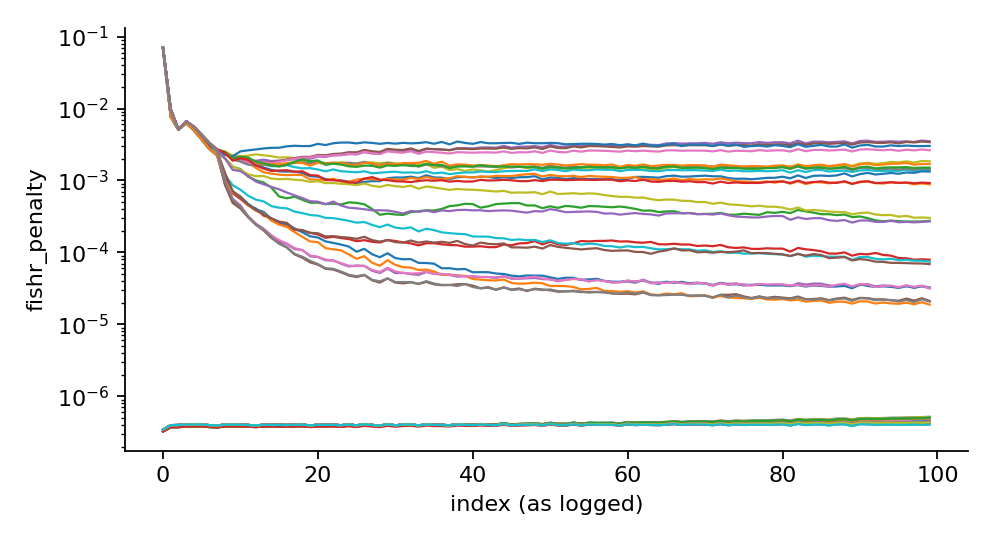
\includegraphics[width=\textwidth]{curve_fishr_penalty.png}
\caption{\texttt{fishr\_penalty}, the mean over seeds per cell.}
\label{fig:curve-2}
\end{figure}
\begin{figure}[tbp]
\centering
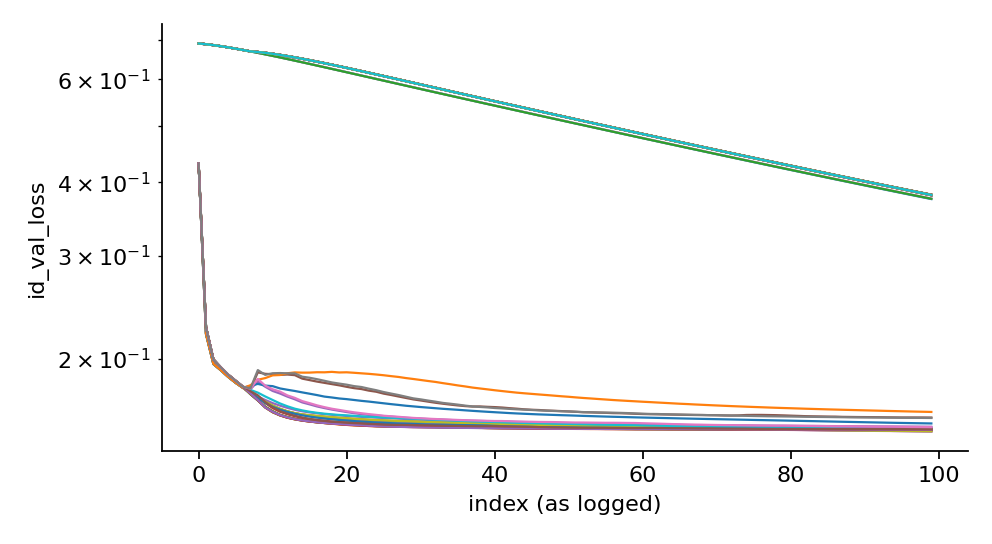
\includegraphics[width=\textwidth]{curve_id_val_loss.png}
\caption{\texttt{id\_val\_loss}, the mean over seeds per cell.}
\label{fig:curve-3}
\end{figure}

\section{Configuration}
The base configuration every run shares (frozen hash \texttt{096095567af4}); factor levels are in \autoref{tab:summary-ood_len_f1}.
{\footnotesize
\begin{verbatim}
task:
  name: ThreeSumDecisionDataset
  value_range:
  - -20
  - 20
  target_range:
  - -75
  - 75
  weight_range: null
  adversarial_range:
  - 40
  - 60
  noise_prob: 0.0
data:
  train_lengths:
  - 4
  - 5
  - 6
  - 7
  - 8
  ood_lengths:
  - 12
  - 16
  - 64
  ood_value_range:
  - -375
  - 375
  ood_noise_range:
  - 40
  - 60
  ood_noise_prob: 0.5
  n_per_length: 20000
  n_eval_per_length: 2000
  curve_eval_limit: 256
model:
  d_model: 64
  n_heads: 2
  num_layers: 1
  dropout: 0.0
  tropical_impl: legacy
optim:
  lr: 0.0001
  epochs: 100
  batch_size: 100
  eval_batch_size: 256
fishr:
  ema: 0.95
  anneal_iters: 1500
  reset_optimizer: true
\end{verbatim}
}
Store: \texttt{campaigns/tropical/ThreeSumDecision/results}.
\end{document}